% \documentclass{article}
\documentclass{book}

\let\cleardoublepage\clearpage

\usepackage[english]{babel}

% Set page size and margins
% Replace `letterpaper' with `a4paper' for UK/EU standard size
\usepackage[letterpaper,top=2cm,bottom=2cm,left=3cm,right=3cm,marginparwidth=1.75cm]{geometry}
\usepackage{graphicx}
\usepackage{xcolor}
\usepackage[colorlinks=true,linkcolor=blue,citecolor=red]{hyperref}
% \setlength{\parindent}{0pt}

% \usepackage{natbib}
\newenvironment{abstract}{}{}
\usepackage{abstract}

\hypersetup{
    colorlinks=true,
    linkcolor=[RGB]{255,34,255},
    citecolor=[RGB]{255,34,255},
}

\title{Towards General and Autonomous Artificial Researcher: Perspective Paper}
\author{Shiro Takagi\footnote{The LaTeX file of this perspective paper is stored on GitHub. The paper is still under active development, and you can review the past update history from the repository. If you have any proposals to improve this paper, please feel free to submit a pull request to the repository. Let's work together to create a better paper! \\ GitHub: \url{https://github.com/t46/research-automation-perspective-paper}. }}

\begin{document}
\sloppy
\maketitle
\tableofcontents

\begin{abstract}
    In this paper, we propose a perspective on the realization of a general and autonomous artificial researcher. First, we discuss the definition of research to clarify the goal we pursue. Second, we review existing literature of research automation to know our current standing point. Third, based on these discussions, we propose what we should to realize a general and autonomous artificial researcher.
\end{abstract}

\chapter{Introduction}

\section{Towards Understanding this Universe}
It has been a long-standing goal of humanity to understand nature, the universe, and the world. Through this intellectual curiosity, mankind has made remarkable intellectual advancements and uncovered astonishing findings about nature. While perfect understanding of this universe may be infeasible, the desire to know as much as possible about as many things as possible in this universe is a shared sentiment among researchers.

However, it seems that there are limitations to achieving this goal solely through current human capabilities. This is because humans have several cognitive constraints when it comes to understanding phenomena. For instance, there is a limit to the amount of information humans can process, and comprehending highly complex, nonlinear, and non-equilibrium systems in their entirety is challenging. Such constraints appear to narrow the scope of nature that can be understood. \textcolor{red}{TODO: update the explanation of cognitive limitation}

Furthermore, there is a possibility that the methodologies of knowledge production employed by humans currently may not be optimal. This is because the research practices we have developed are heavily influenced by historical and societal factors. Many of these practices have emerged in a relatively short span of history, and there is still a vast unexplored territory in the methods of conducting research.

We believe that artificial intelligence capable of autonomously conducting all research holds great potential in overcoming these challenges and getting closer to the goal. Firstly, AI is not constrained by a physical device like the human brain, enabling processing speeds and capacities that are orders of magnitude beyond human capabilities. Secondly, by optimizing AI for knowledge production, it becomes possible to generate knowledge more efficiently, without being constrained by extraneous factors commonly encountered in human research. Lastly, and most importantly, AI has the potential to possess a different understanding of nature compared to humans. Moreover, AI might have the capacity to comprehend nature more extensively than humans. If that's the case, it seems essential to develop autonomously researching artificial intelligence if one aims to acquire as much knowledge as possible about this universe. Therefore, we propose the pursuit of autonomous AI researchers to realize these possibilities.

\section{Purpose of this Perspective Paper}
The purpose of this perspective paper is to provide a stepping stone towards achieving a general and autonomous artificial researcher as quickly as possible. It aims to offer information that enables all those pursuing this goal to focus on essential issues, avoid reinventing the wheel, and maximize their own potential. This is because we believe that enabling the full potential of brilliant researchers worldwide is the most crucial for accomplishing this objective.

To achieve the purpose of this perspective paper, we will discuss three key points in chapters 2, 3, and 4, respectively: What is the goal, where are we currently standing, and what to do to achieve the goal. First, in chapter 2, we will delve into the discussion of ``What is the goal'' to make the common objective clearer for everyone involved. By doing so, researchers and engineers all over the world are able to devise methods to achieve this goal even before looking at our proposals in this paper. Furthermore, this discussion aims to clarify the limits and possibilities of a general and autonomous artificial researcher. Specifically, we will thoroughly discuss ``What is research?'' as it is essential to understand what a ``general'' artificial researcher entails. Starting with the definition of research, we will examine the functions that various research activities serve and discuss the implications of achieving this through artificial intelligence.

Next, in chapter 3, we will discuss ``Where are we currently standing'' to work towards a state where researchers pursuing research automation no longer need to gather preliminary information on their own. This is expected to enable new researchers engaged in research automation to concentrate on the actual tasks they should be working on and reduce the risk of reinventing the wheel. To accomplish this, we conduct a literature review on research automation. We will organize studies related to research automation, discuss their relationships and current status. In this survey, we will strive for as much comprehensiveness as possible, including anything relevant to research automation, no matter how superficial, as we believe that once researchers become aware of the research area, they can delve deeper into specific aspects on their own. Additionally, we observed a lack of information sharing among various individual efforts related to research automation, and by addressing these diverse approaches in a unified manner within one paper, we aim to promote information exchange between different fields.

In chapter 4, we will present our proposals on ``What to do to achieve the goal.'' Building upon the clarity of the goal from chapter 2 and the understanding of the current state from chapter 3, we will discuss how to bridge the gaps between them. We will also explore the directions and specific approaches for research and development, suggesting the policies and avenues that may be most effective. Through these discussions, our aim with this paper is to providing useful information for as many individuals striving for research automation.

Chapter 2, 3, and 4 focus on creating a general and autonomous artificial researcher, with only minimal suggestions about its impact on society once completed. Chapter 5 will address issues such as the impact on society from the perspective of "alignment." Furthermore, we will discuss how alignment can play an essential role not only in mitigating the risks of AI but also in automating research.

\section{Pursuing Better Research}
Please emphasize once again that what we are aiming for is to achieve a better way of knowledge production. The realization of general and autonomous artificial intelligence is a means to that end. Therefore, even if certain research practices are widely adopted at present, we will strive for better methods if they are not essential for knowledge production and if there are superior alternatives. In other words, we propose to pursue the realization of artificial intelligence that enables a different and improved way of knowledge production, rather than simply automating the current research practices.

While the practices of research developed by humans are highly sophisticated, robust, and productive, it is not necessarily true that all of them have reached the absolute optimum way of doing research. Firstly, research practices are strongly influenced by history and society. For example, peer review is widely accepted today, but it is said to have gained such dominant status because foundations in Cold War-era U.S. demanded peer review to ensure accountability \cite{baldwin2018scientific}. Moreover, the fact that research outcomes are still represented in the form of papers is clearly a remnant of the era when print was predominant. These practices might have been optimal under the social conditions and technologies of that time, but they may not necessarily be optimal in the present, as society has changed a lot. Additionally, meeting societal demands does not always lead to the optimization of knowledge production. Secondly, it seems that we sometimes lack a widely shared understanding of how to optimally carry out certain aspects of research. For instance, it is important to formulate good research questions and hypotheses, but there are still many aspects about how to do this effectively that remain unclear, and it appears to rely heavily on individuals' tacit knowledge. In such a situation, simply replacing current practices with machines may not guarantee a good knowledge production process. Thirdly, as Nielsen and Qiu say \cite{nielsen}, it is believed that we have only explored in a very limited subspace in the space of possible research practices. The establishment of current research practices is a very recent event in human history, and we may not yet have arrived at the optimum way of research. \textcolor{red}{TODO: Add examples.} Finally, as we mentioned above, current research assumes that humans are the main creators and consumers of knowledge. This naturally imposes human cognitive constraints, which may significantly limit the range of activities that can be conducted for knowledge production. Based on these reasons, we aim to progress the discussion in a way that allows us to identify what is fundamentally essential for knowledge production, while also drawing inspiration from the positive aspects of past practices. We will not be bound by the current approaches but instead strive to clarify what is truly crucial for research.

\section{Call for Cooperation}
I would be delighted if all of you could contribute to writing this research paper. The initial draft of this paper was created by a novice machine learning researcher named Shiro Takagi. We have made efforts to write the text as carefully as possible, but due to his limited research experience, He may not be able to provide profound insights into the topic, and there might be inaccuracies in his understanding of fields that are not his expertise. In particular, the literature review chapter prioritizes comprehensive coverage of the literature, which means that the evaluation of individual references might not be appropriate. Also, there are naturally limitations and biases regarding the scope of papers that can be covered and the research areas targeted. Therefore, if you find any errors, missed literature, or points for improvement in the paper, we would be grateful if you could let us know.

The manuscript is being managed on GitHub\footnote{\url{https://github.com/t46/research-automation-perspective-paper}}, and contributions from everyone to the paper are welcous. The version you are currently reading is a provisional one, and we plan to continue updating it regularly. If you have any suggestions for modifications, it would be incredibly helpful if you could submit a pull request to the repository.

Moreover, this paper is licensed under the OO license, so feel free to make any modifications you see fit. If you wish to follow the main structure, you can fork the repository, or if you have a different approach in mind, you can create an entirely new project.

We hope this paper can contribute in some way to the advancement of automation in research. Thank you.


% Additionally, this paper is intended to be updated on an ongoing basis. If you find points that you think are lacking or inaccuracies in understanding, please send a Pull Request on GitHub. Based on that, we will revise the content of the paper as needed.

% \section{Others}

% The purpose of this perspective paper is to discuss the possibility of automating this activity of research, that is, the realization of intelligent agents capable of conducting research autonomously. After summarizing attempts at research automation so far, we intend to present our personal perspective on promising ideas, necessary elements, and ways to proceed in order to create artificial researchers. In particular, this paper is aimed at machine learning researchers and developers, with the goal of increasing the number of colleagues aiming for research automation by providing concrete possible actions.

% One thing to note here is that our aim is not to automate or substitute the current research tasks, but to create intelligent agents capable of conducting research. In other words, as long as it is research, automated research may at first glance seem to be far removed from the current research activities. This is because the current research activity may not necessarily be the absolute optimal form in light of its purpose. 

% First, the optimal form is always influenced by the context of history. Of course, the optimum in the era when letterpress printing was mainstream is different from the optimum in the era when the Internet became infrastructure. Research itself has changed its form over time, and the optimal form of research in the present or future can naturally change. Moreover, as Nielsen and Qiu say \cite{nielsen}, it is believed that we have only explored a very limited range regarding the practice of research. The establishment of current research practices is a very recent event in human history, and we may not yet have arrived at the optimum way of intellectual production. Furthermore, current research assumes that humans are the main creators of knowledge. This naturally imposes human cognitive constraints, which may significantly limit the range of activities that can be conducted for knowledge production. 

% Therefore, instead of thinking about how to automate and streamline current tasks, we discuss the possibility of realizing intelligent agents that can autonomously perform the fundamental and core elements of research activity in a more optimal form, and what is necessary for this.

\textcolor{red}{TODO: Add lots of high-level illustration}

\chapter{What is the Goal?}
\label{chapter-what-is-research}

To reiterate, \textbf{the proposition put forward in this paper is to strive for the realization of general and autonomous artificial researcher}. Autonomy refers to the level of human intervention and design involved. For instance, a system that requires humans to explicitly provide a set of hypotheses has lower autonomy compared to one that allows the machine to discover them on its own.  Generality refers to how many research fields a single automated research system can handle. For example, a system capable of conducting research in both physics and history is more general compared to a system limited to either one.

While it might be easier to grasp what a more autonomous system is, the challenge lies in defining what a general artificial researcher is. This is because we need to comprehend what it means for a system to be capable of both physics and history research, for example. Therefore, to create a general artificial researcher, it seems necessary to first define what research itself is. By discussing what constitutes research and what is required to conduct it, we may uncover the abilities that the system must possess. Hence, the following sections will explore the fundamental nature of research.

\begin{figure}[htb]
    \centering
    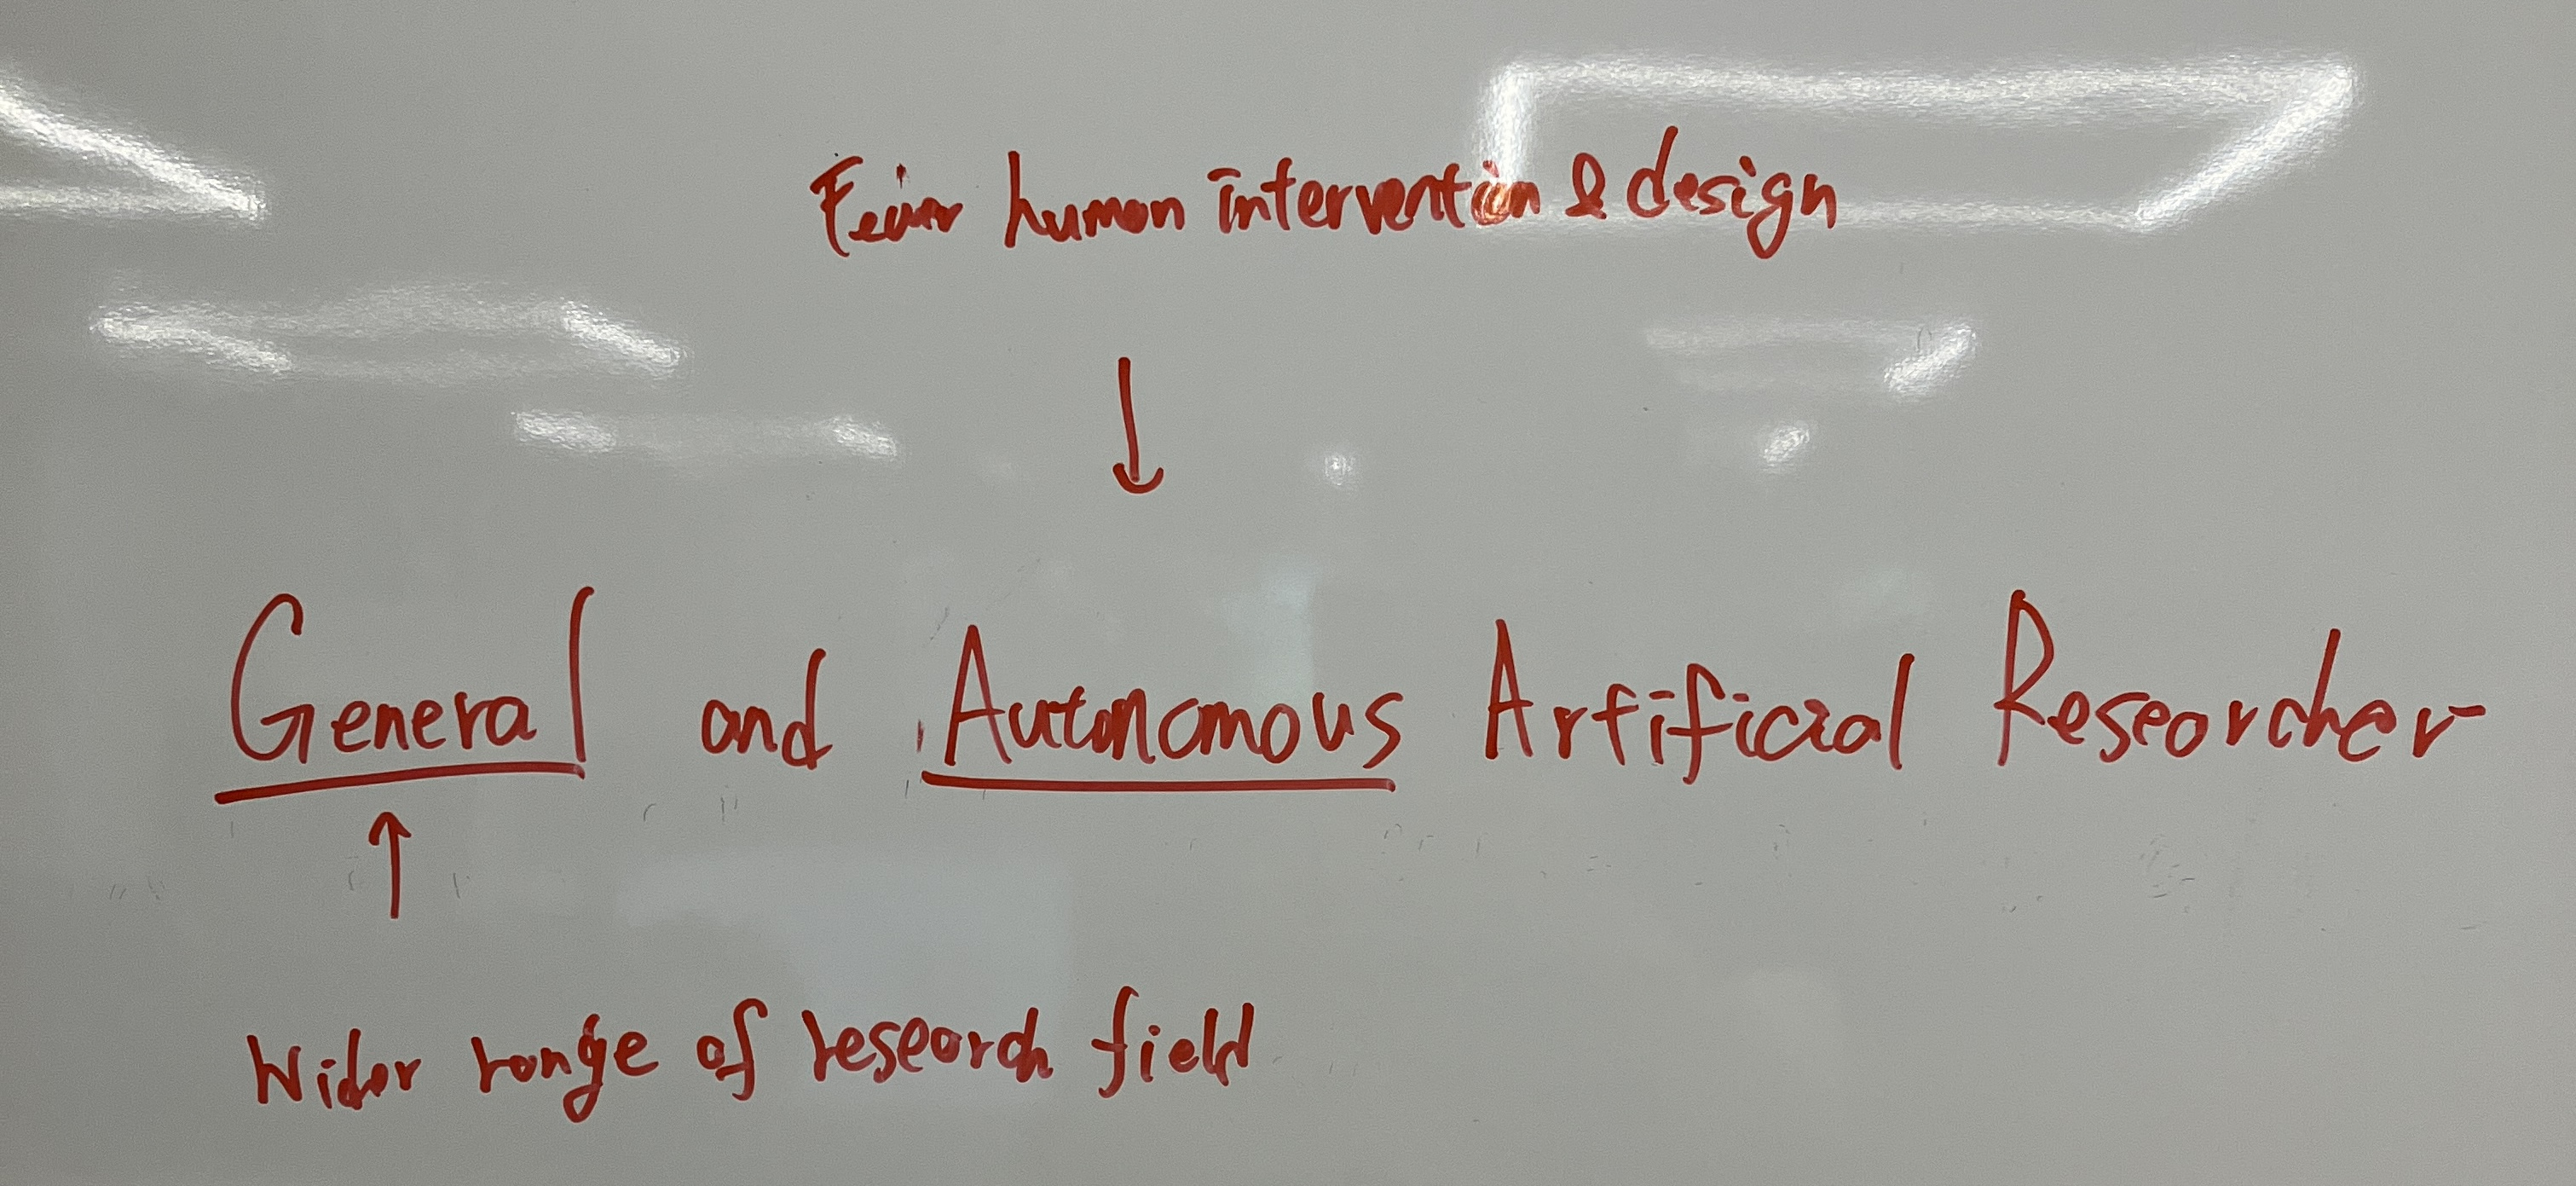
\includegraphics[width=\linewidth]{figs/goal.jpg}
    \caption{General and Autonomous Artificial Researcher}
    \label{fig:goal}
\end{figure}

\section{What is Research?}
To create an agent capable of conducting research autonomously, it is crucial to understand what research is in the first place. Therefore, in this section, we would like to discuss the characteristics of what is called research.

However, our aim here is not to identify a universal, historically independent, and absolutely singular definition of what research is. It seems almost impossible to specify such a thing \cite{chalmers2013thing,sep-scientific-method}. We do not totally believe that we could provide an answer to a question that has yet to be resolved even within the philosophy of science.

Rather, our goal is to endeavor to describe various characteristics of research to the extent that it can provide a starting point for engineers and information scientists who aim for autonomous research capabilities. To that end, we first discuss a possible working definition of research.

\subsection{Research as Knowledge Production}

One commonly mentioned definition of research is the act of generating new knowledge. For instance, research of mathematics create unknown proofs of theorems, physics elucidates unknown natural laws, and engineering produces blueprints for never existed things. We will adopt this definition as the working definition in this paper. In particular, we consider that \textbf{research is producing new knowledge for members of a society.} Therefore, whenever we refer to research in the following, please interpret it as discussing the novel knowledge production for a ssociety. \textcolor{red}{TODO: Add discussion}

\begin{figure}[htb]
    \centering
    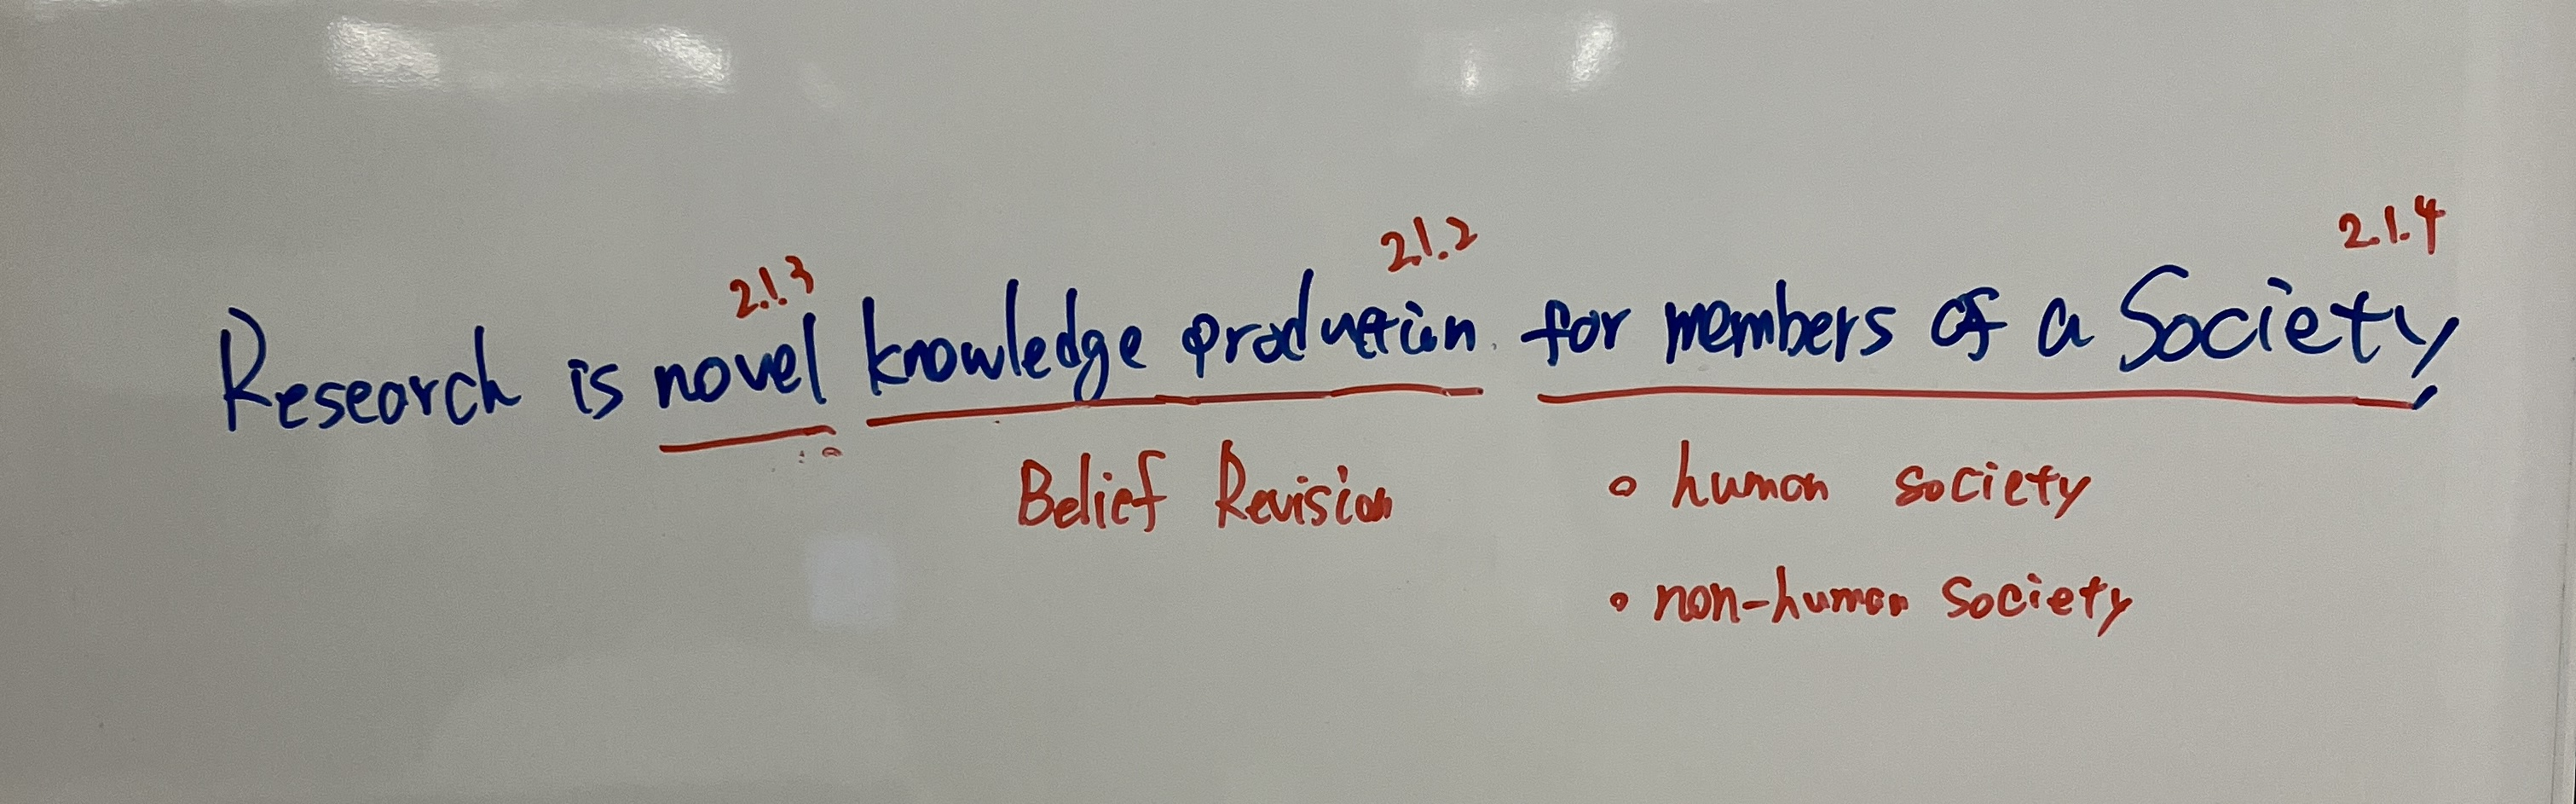
\includegraphics[width=\linewidth]{figs/definition.jpg}
    \caption{Definition of Research}
    \label{fig:definition}
\end{figure}


\subsubsection{Some Notes on Research and Science}

The reason why we deliberately use the word ``research'' instead of ``science'' is because we want to include fields like humanities and arts, which are not typically referred to as science, within the scope of automation in the long run. Science refers to a methodology for generating knowledge, and we believe that new knowledge is not necessarily produced only by scientific methods. We believe that so-called humanities and arts also share the commonality of producing new knowledge. Therefore, the definition of generating new knowledge can be said to encompass these fields as well.

Of course we admit that science is an extremely precise and robust  framework for knowledge production. Because of its power and popularity, most of the existing analysis on research is about science. Therefore, although we try not to be limited to science as far as we can, our understanding of research has been significantly influenced by the previous work about science. Thus, our discussion would be centered around the discussion of science. We would like to explore the analysis towards the automation of research other than science in the future.

\subsection{Knowledge Production as Belief Revision}
We have defined research as the generation of new knowledge. Now, what exactly is knowledge, and what does it mean to produce knowledge? We will explore this question in this section. 

Defining knowledge and knowledge production rigorously is a philosophical debate that has not yet been settled \cite{sep-epistemology}, and we won't delve into it deeply here. Instead, we would like to provide some primitive ideas as machine learning researchers that can serve as a starting point for further discussions on the automation of research.

\subsubsection{Knowledge as Belief}
The question of what is the thing called knowledge has been a subject of debate for a long time in the field of \textit{epistemology}, which is one of the branches of philosophy. In epistemology, knowledge has been traditionally considered to be \textit{justified true belief (JTB)} \cite{sep-epistemology}. The term ``true'' is difficult to define rigorously, but for the purpose of discussion, let's think of it as something being fact. ``Belief'' can be provisionally understood as someone's thought or conviction about something. And ``justified'' means that it is deemed reasonable to hold such a belief. The meaning, necessity, and sufficiency of justification has been discussed in epistemology as a central point of contention. Since we are not well-versed in epistemology, we will refrain from delving into detailed discussions on that topic as it would go beyond the scope of this paper.

Of course, there is much debate about whether JTB truly is knowledge, and many philosopher agree that JTB is not the sufficient condition of knowledge. While these characteristics are not be sufficient conditions, there is generally some agreement that they seem to be necessary. Also, as even epistemological discussions revolve around these notions, they seem to provide a reasonable starting point just for the purpose of our discussion. Therefore, for the sake of further argumentation, let's tentatively understand the generation of knowledge as the process of justifying, validating, or confirming beliefs about a truth in some form.

\subsubsection{Research as Belief Revision}
We are not sure if it is necessary for JTB to be strictly true in order for an action to be considered research. Nevertheless, intuitively, it seems somewhat valid as a description of research that research is updating a belief. For example, let's consider a scenario where a hypothesis is proposed for a certain phenomenon, and then it is subjected to a test. This is a common practice in research. Now, suppose that through this testing, the hypothesis has been validated. This means that as a result of the test, our belief that the hypothesis is true has been strengthened. Therefore, the view that research involves the update of belief seems to be reasonably valid.

% In the nature of research, which aims to generate new knowledge, it is necessary to engage in inference and justification regarding the unknown. Even if a hypothesis is not explicitly stated, some form of implicit hypothesis generation and testing should occurs in research. Therefore, the view that research involves the update of belief seems to be reasonably valid.

Let us explain a bit more about the reason why we deliberately say ``our belief that the hypothesis is true has been strengthened'' without just claiming that ``hypothesis turned out to be true.'' This is partly because, in almost all fields that rely on empirical methods, except for deductive disciplines like mathematics and logic, it is often impossible for verification to definitively determine if a hypothesis is true or false. Most research evaluates the validity of a hypothesis based on observed cases, relying on inductive reasoning \cite{sep-scientific-method}. However, inductive reasoning is believed to be unable to determine the truth or falsehood of propositions without assumptions, as deduction does \cite{sep-induction-problem}. Even in such situations, we can argue that the evidence obtained through verification makes us feel more confident in our hypothesis. This applies to both empirical and deductive research. Thus, we say that a hypothesis became truth but that our belief is updated.

We don't believe that because inductive reasoning doesn't rigorously determine truth or falsehood in the same way deduction does, it renders the reliance on inductive reasoning meaningless. Because the assumptions that are said to make the inductive reasoning valid feel extremely natural to us and leave little room for doubt. As an example, it is said that we need to assume that ``under the same conditions, the same phenomenon will continue to hold'' (principle of uniformity of nature) \cite{sep-induction-problem}, which is an extremely intuitive assumption without which we could hardly even go about our daily lives.\footnote{The problem of what assumptions make us inductive reasoning consider rational is an extremely difficult unanswered philosophical issue, which is beyond the scope of this paper. Thus, we will refrain from delving into the details here and leave it for future discussion. We understand that justifying the validity of inductive reasoning based on our experiences would be circular reasoning, and we cannot guarantee that these assumptions always hold ever. However, the extremely strong beliefs that feel justified based on our perception and experience seem much more reliable than some random conjecture. This is enough for us to feels that relying on inductive reasoning is meaningful.} 

For the same reasons, we do not believe that the concept of belief being subjective makes it unsuitable for characterizing research. What we want to emphasize here is that research can be seen as linking or replacing the weak belief in the plausibility of newly conceived hypotheses with such extremely strong beliefs. For example, believing in the effectiveness of statistical methods is strongly related to believing in the effectiveness of inductive reasoning. Therefore, if the validity of a hypothesis is confirmed using statistical methods, we would believe it as highly reliable. Hence, considering research as the updating of beliefs can be reasonably felt, and we don't intend to argue that research is meaningless just because it is the belief revision.\footnote{We naively explored the differences in strength within beliefs, the idea that beliefs rooted directly in perception are more robust, and the notion that anchoring a belief on those foundations enhances its reliability. However, the question of how justified beliefs are grounded and the nature of their structure is a highly complex problem with extensive discussions  \cite{sep-epistemology}. If we understand it correctly, our position may align somewhat with what is called \textit{empirical foundationalism}. Properly engaging with these discussions and considering where to seek the foundations of knowledge seems crucial in debating the new manner of generating knowledge. However, due to our limited philosophical knowledge and the ability to delve deeper into philosophical discussions, this paper will not further pursue these arguments.}


% Therefore, while we don't know what exactly constitutes the basis of inductive reasoning, it would seem to be a deeply rooted and unwavering belief that is grounded in our perception and experiences. 

% \textcolor{red}{TODO: Add excuse for empirical foundationalism}
% The idea that there is ``strength'' in beliefs may be related to a position called \textit{foundationalism} in epistemology, which claims that ``\textit{our justified beliefs are structured like a building: they are divided into a foundation and a superstructure, the latter resting upon the former. Beliefs belonging to the foundation are basic. Beliefs belonging to the superstructure are nonbasic and receive justification from the justified beliefs in the foundation.}'' \cite{sep-epistemology}. In particular, we believe that the more fundamental beliefs to which these beliefs belong are rooted in human perceptual experience and empirical knowledge. This position is commonly referred to as \textit{empirical foundationalism} \cite{sep-epistemology}.



\subsubsection{Alternative Definition of Research}
We have adopted the definition that knowledge is JTB, which implicitly assumes that the generation of knowledge, i.e., research, aims at acquiring a truth. However, there is also a position that evaluates beliefs not by whether they approach truth but by whether they are useful in some sense. This position is known as \textit{pragmatism}. From this perspective, it could be possible to argue that the outputs of current machine learning models, for example, may be considered knowledge since it shows high predictive performance. In this sense, this position views is highly compatible with contemporary statistical machine learning \cite{otsuka2022thinking}.

As such, this pragmatism presents a different view of research from that of majority of researchers, and it could be seen as advocating a redefinition of the act of research. Many researchers may not accept this view. Nevertheless, in recent years, large language models have made rapid advancements and have produced many ``useful'' outcomes in research, which has made the debate on whether to consider their outputs as knowledge much more relevant and realistic than ever before.

In this paper, we take the position that knowledge is JTB, and research is an endeavor to approach a truth. Therefore, we will not address this issue in the following sections that much. However, we must seriously consider the implications presented by large language models and delve deeper into the discussion of how we define research, what constitutes research, and what purpose research serves. We believe that this is of utmost importance for our society.

\subsection{Novelty of Knowledge}
As defined earlier, research is considered to be the process of producing ``new'' knowledge or transforming the unknown into the known. No matter how firmly a belief is confirmed, if it is already known, it cannot be called research. Therefore, it seems necessary to carefully discuss what it means for knowledge to be unknown or novel.

% We said in the paragraph above that ``research is the process of transforming the unknown into the known.'' However research can also be seen as the updating of beliefs, as we have explained. Therefore, the binary depiction of an object suddenly transitioning from the states of unknown to known does not seem appropriate. Rather, it seems more reasonable to consider that beliefs continuously change and we just call some group of belief states unknown and others known, for convenience.

% We don't know precisely what it means to be unknown. This is a difficult problem, but let's consider it naively. 
We consider a knowledge to be unknown when for a question a subject lacks any hypothesis which he/she has a JTB that the hypothesis is true. For example, we do not have the answer to the question of ``How to realize an artificial general intelligence.'' So the knowledge of ``the way to realize an artificial general ingelligence'' is unknown. \textcolor{red}{TODO: Add explanation}

The expression ``unknown'' could be more appropriately expressed as ``high degree of unknownness''. Because knowledge production is a continuous concept of belief updating, therefore, unknownness is also a continuous concept. In reality, there are multiple hypotheses with varying degrees of certainty concerning a particular question. The state of knowledge being unknown can be expressed as not having any hypothesis among these hypotheses with a particularly strong level of justified certainty.

% First, research begins with a particular question. The state of not knowing the answer to this question is what we consider the state of being unknown. In other words, it can be thought of as a state where we don't know what the candidate hypotheses, which are the potential answers, are like, or a state where we know the candidate hypotheses but don't know their plausibility. These are states where we have not been able to find hypotheses or sets of hypotheses that can be assigned a particularly high degree of confidence from the set of potential answers to a given question. Therefore, provisionally and casually, it might be said that the state of ``not having highly confident beliefs (or a set of beliefs) for a particular question'' is unknown, and the state of having highly confident justified beliefs is known.

% Of course, there are issues with this clarification. For example, it is unlikely that we can select a single highly confident hypothesis from the entire set of possible hypotheses. Also, rather than feeling equally confident about all possible hypotheses, it seems that we implicitly distinguish between hypotheses that seem relevant and those that do not. Furthermore, it is unclear to what extent we consider a state to be unknown based on the degree of confidence. However, these are highly challenging philosophical discussions, so we will refrain from delving further into them and, for now, would like to conclude with the vague and provisional definition above and move on to the next topic.

\subsection{Publicity of Knowledge}
\subsubsection{Knowledge as Human Knowledge}
The knowledge generated through research seems to be required to be knowledge for humanity. In reality, even if it is a strong belief, one person's belief is not recognized as knowledge unless other researchers gain a similar level of conviction from the research. Beliefs, knowledge, and understanding are indeed subjective concepts by nature, but it seems that we demand that they go beyond subjectivity and become comprehensible to others in some form. 

Therefore, to generate knowledge for humanity, it is necessary to update the beliefs of all humanity. Since updating the beliefs of all humans is impractical, realistically, we focus on updating the beliefs of a subset of individuals. For example, knowledge in physics is considered as such when it instills a similar conviction in researchers studying physics. Even in this case, knowledge is generated as something potentially understandable to a considerable number of people. This also means that the generated knowledge is not only for the society at the time of its production but also for the broader humanity, including future human societies. For instance, it might be challenging for a high school student to determine whether the research outcomes in physics qualify as knowledge. However, by studying physics extensively, there is a possibility of eventually comprehending cutting-edge research in the field. Moreover, it is obviously impossible for different individuals to have exactly the same belief states, so as long as a justification can update the beliefs of different individuals in a similar direction in some way, we think it sufficient to be regarded as updating shared beliefs.

% Therefore, we believe research is the act of not only changing an individual's belief but also changing multiple individuals' beliefs. 

% Although we don't think it is possible for multiple people to hold exactly the same belief or for their beliefs to change in exactly the same direction, we at least need to use a way to change a collection of human beliefs in a similar direction.

We believe that humans achieve the updating of shared beliefs by converging a hypothesis's belief in truth to a highly robust conviction that is universally held among humanity, regardless of individual differences. This robust belief refers to those beliefs rooted in our biological structures and perceptions acquired through the processes of evolution and development, as briefly introduced in the preceding section. For instance, beliefs such as the validity of logical reasoning, the uniformity of nature, and the tendency to find something more credible with an increase in observations fall into this category of beliefs. 

The objectivity of research seems to arise from the demand for research to produce knowledge for humanity.\footnote{We admit that finding the basis of objectivity of research is a challenging philosophical issue. Please note that what we have stated here is merely the humble intuition. } Because of this requirement, researchers conduct research with extreme precision and caution. Although we often casually ``validate'' hypotheses in daily life, these activities are generally not considered research because they lack the meticulousness and objectivity that are integral to the research process. Research is designed and executed with much greater care and precision than everyday ``validation'' activities. This serves as one of the justifications for the knowledge produced through research being reliable.
% And we believe that we achieve this by reducing hypotheses to strong convictions that everyone, regardless of individual differences, possesses as human beings. For example, assumptions underlying inductive reasoning, as we described earlier, will fall into this category. Another strong conviction humans believe in is that the more we observe an increasing number of results derived from a certain hypothesis, the more reliable and certain that hypothesis feels. Research need to be objective because it's required to generate knowledge for humanity, and we believe it is because we strive to reduce hypotheses to such strong convictions that it is called objective. 

Furthermore, seeking public accessibility in knowledge implies that the expressions of knowledge and the process of knowledge production should be understandable to everyone. For instance, in human societies, knowledge is often expressed through language. This is because language serves as a highly universal means of conveying information that a significant number of people can comprehend and handle. Similarly, the process of knowledge production is also conveyed through language.

\subsubsection{Knowledge as Agents' Knowledge}
We mentioned that research is generating knowledge for humanity. However, this is merely because humans have been the ones conducting research thus far. We believe that in principle there could be knowledge for beings other than humans and hence research for them as well, even if the knowledge may not resemble human knowledge on the surface. Let's consider a group of agents, each capable of holding certain belief states and having some level of similarity, which allows them to hold a strong common belief. In the previous explanation, beliefs were not required to attribute a continuous degree of confidence to propositions with truth values. Therefore, it is possible to construct such a scenario. In this case, if these agents have a way to ground their the belief that a certain hypothesis is true to a shared belief, then this can be regarded as research within that society. Therefore, we have defined research as the act of producing new knowledge for members of a society, which is not necessarily human society but also includes societies of non-human agents.

\begin{figure}[htb]
    \centering
    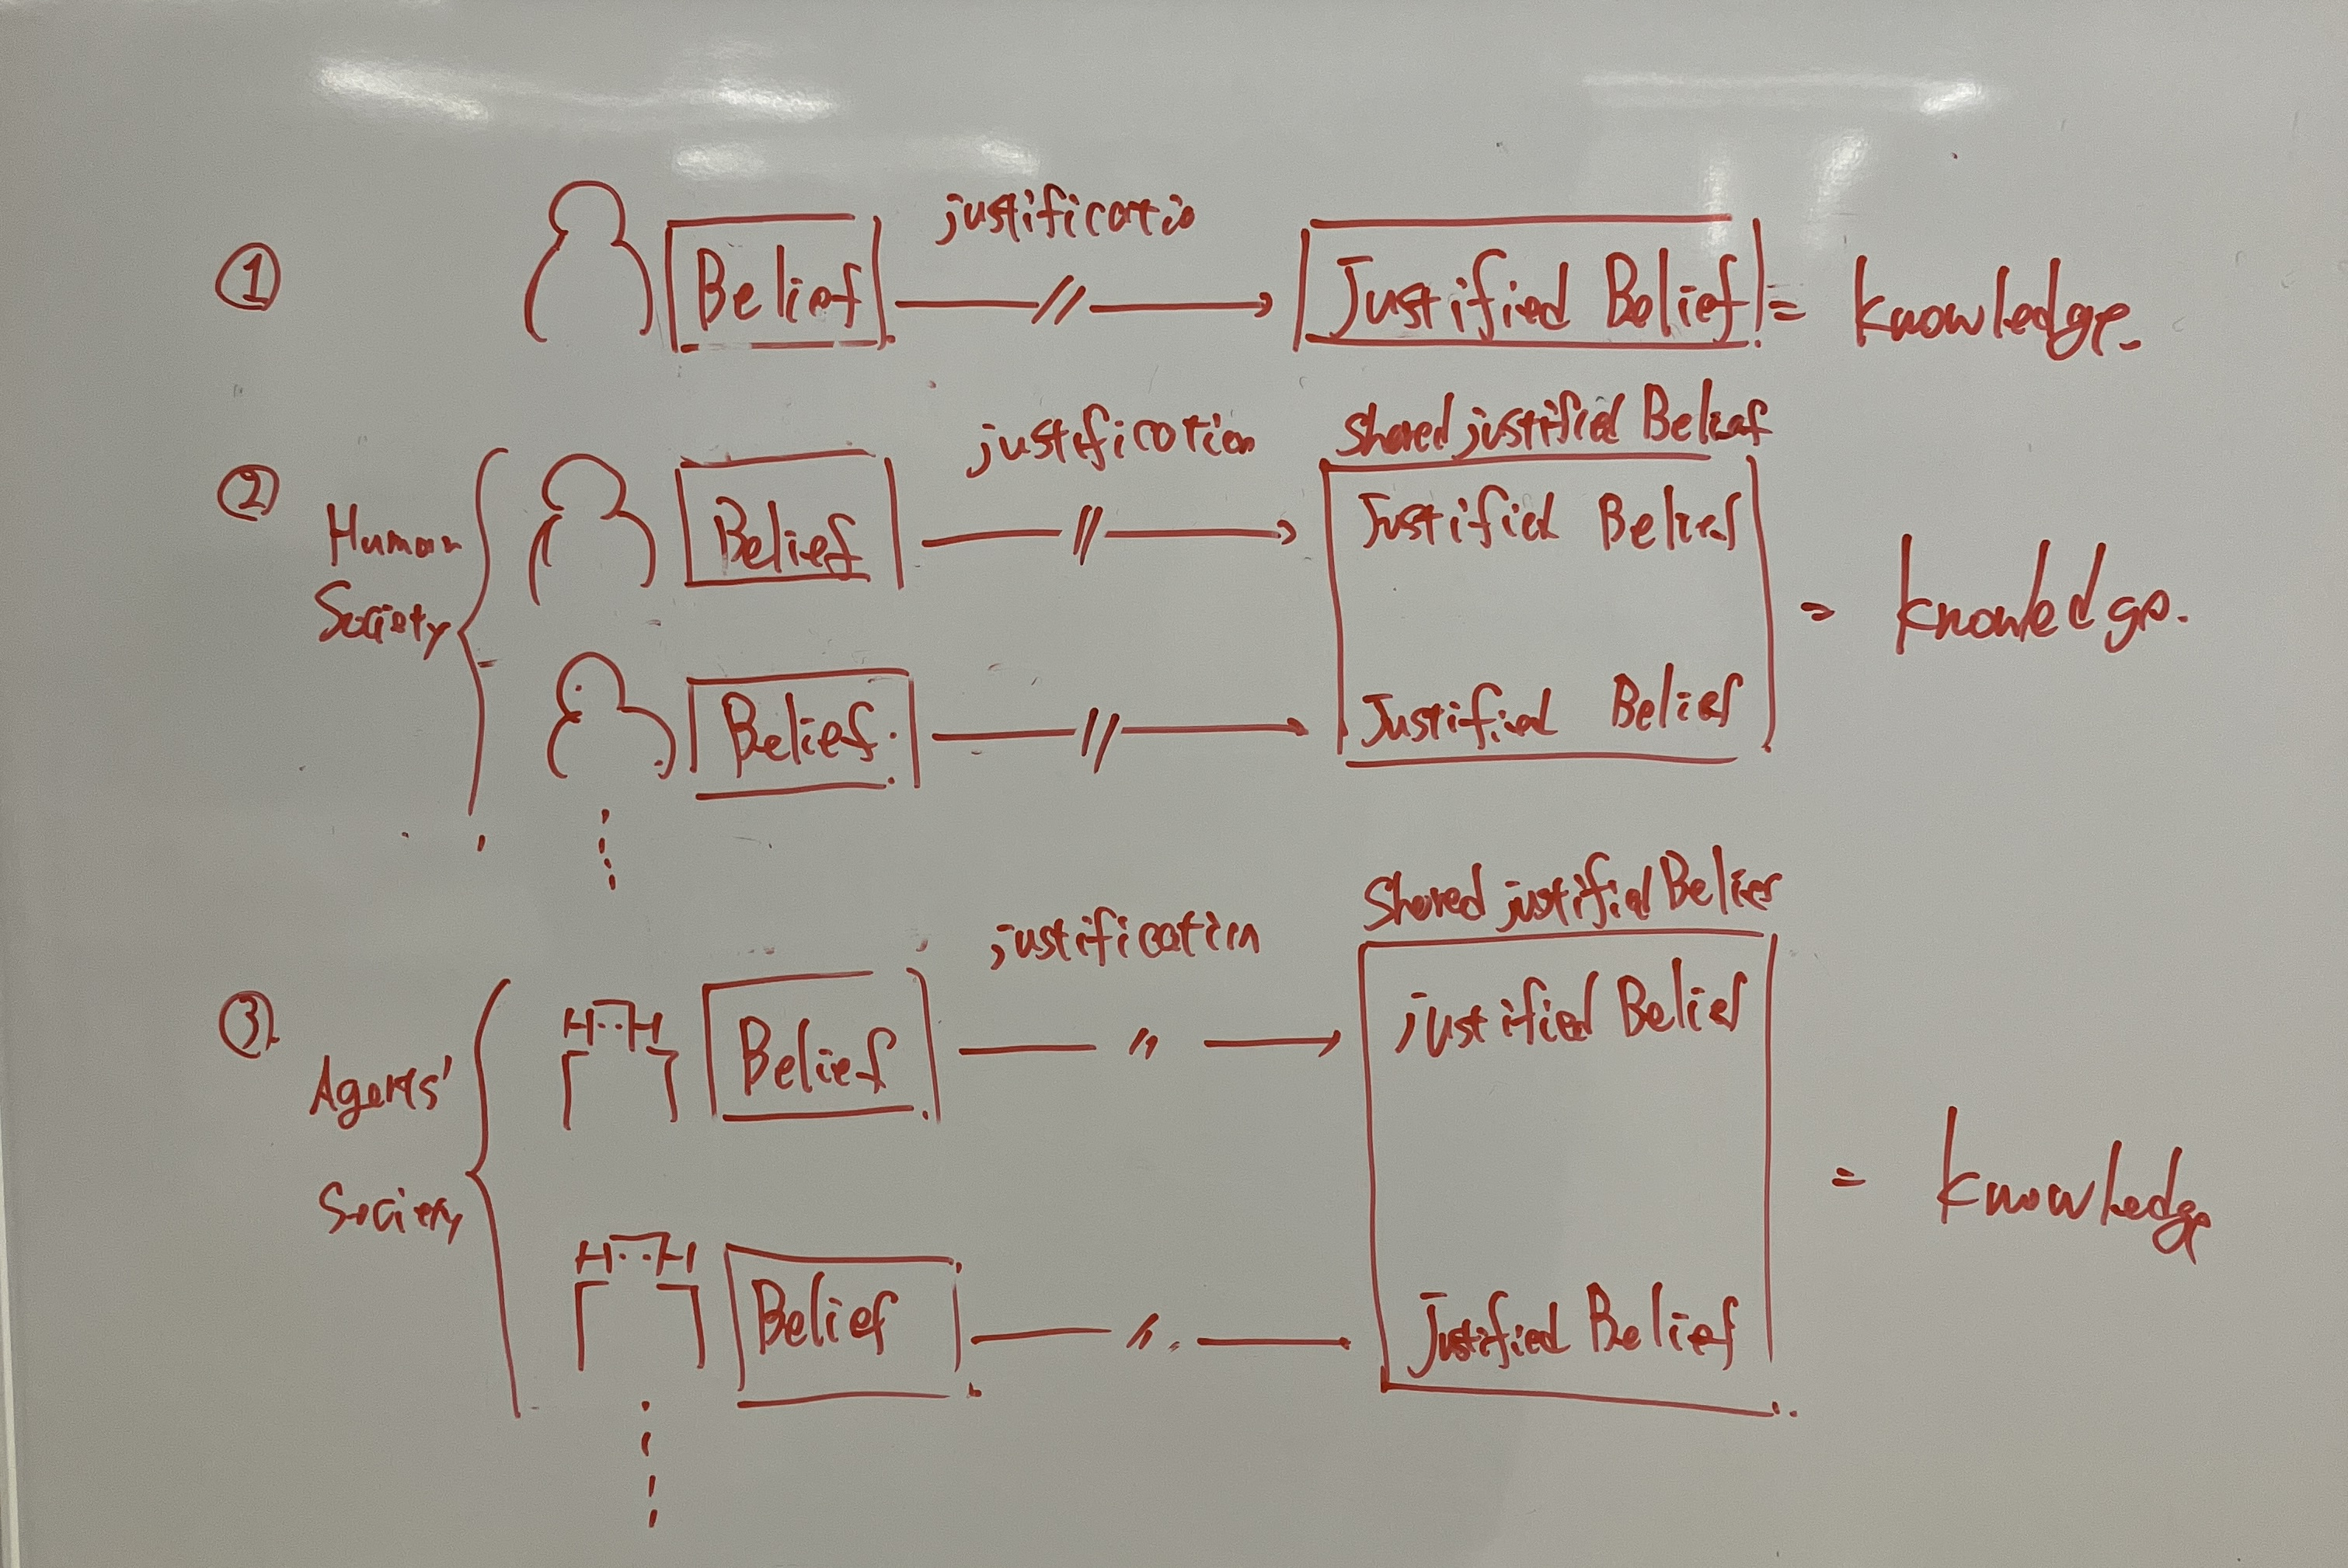
\includegraphics[width=\linewidth]{figs/shared_belief_revision.jpg}
    \caption{Belief Revision}
    \label{fig:definition}
\end{figure}

This fact seems to lead to at least two important implications for artificial researchers striving to understand nature. Firstly, it suggests that a knowledge production system in this sense could potentially produce utter nonsense for humans. As repeatedly mentioned, for a belief to be considered knowledge for a human, it needed to be justified in a way that is ``acceptable to humans.'' This has been achieved by grounding the belief in shared beliefs that humans strongly hold. Therefore, even if a certain group of agents grounds their justifications in solid shared beliefs, it would be mere gibberish for humans if it is not shared among humans. In other words, there may arise a problem of incommensurability \cite{kuhn1962} in beliefs between human society and the society of agents. 

This implication means that if we want non-human agents to produce meaningful knowledge for humans, we need to ground it not in their shared beliefs but in human shared beliefs, or somehow ensure a commonality between these two sets of shared beliefs. If we aim for the former, the non-human agents may no longer be considered as conducting research in the same sense as humans. Additionally, regardless of whether we pursue the former or the latter, the problem remains of how to impart human shared beliefs to these agents, which is a fundamentally challenging issue. This issue is essentially related to the problem of aligning human values with AI, and it is an extremely difficult problem. We shall discuss this point separately.

Certainly, even if we could share belief systems, if knowledge or the processes involved in acquiring knowledge were expressed using entirely incomprehensible systems for humans, it would still be meaningless to us. Therefore, if we seek to generate knowledge that is practically meaningful to humans, it seems essential for both humans and these systems to utilize, at the very least, a common representation format for knowledge, such as human language.

The second implication is that a knowledge production system in this sense does not guarantee generating knowledge meaningful for understanding nature. We believe that the reason mere belief updates have led humanity to such a rich understanding of nature is that our shared beliefs are products of interactions with nature. As a species, humans have spent vast amounts of time interacting with and modifying their bodies to survive in nature. Our beliefs are naturally formed in such contexts, and the beliefs we currently possess are likely advantageous for living in nature. In other words, the essential information for explaining and predicting nature is already internalized in our strong beliefs. It is precisely because we can trace these beliefs back to such interactions that we have been able to produce knowledge that deepens our understanding of nature. Now, suppose an agent has had no interactions with nature whatsoever until now. In that case, it seems highly unlikely that such an agent could acquire beliefs that are in harmony with nature. This goes beyond merely stating the importance of embodiment for AI. It suggests that an immense amount of interaction and learning, enough to form highly strong beliefs and internalize nature, is required and that learning these elements are inevitable for comprehending the natural world. Therefore, to induce non-human agents to produce knowledge useful for understanding nature, even if it is not exactly the same as humans', they must possess beliefs that are robust and compatible with patterns in nature.

\begin{figure}[htb]
    \centering
    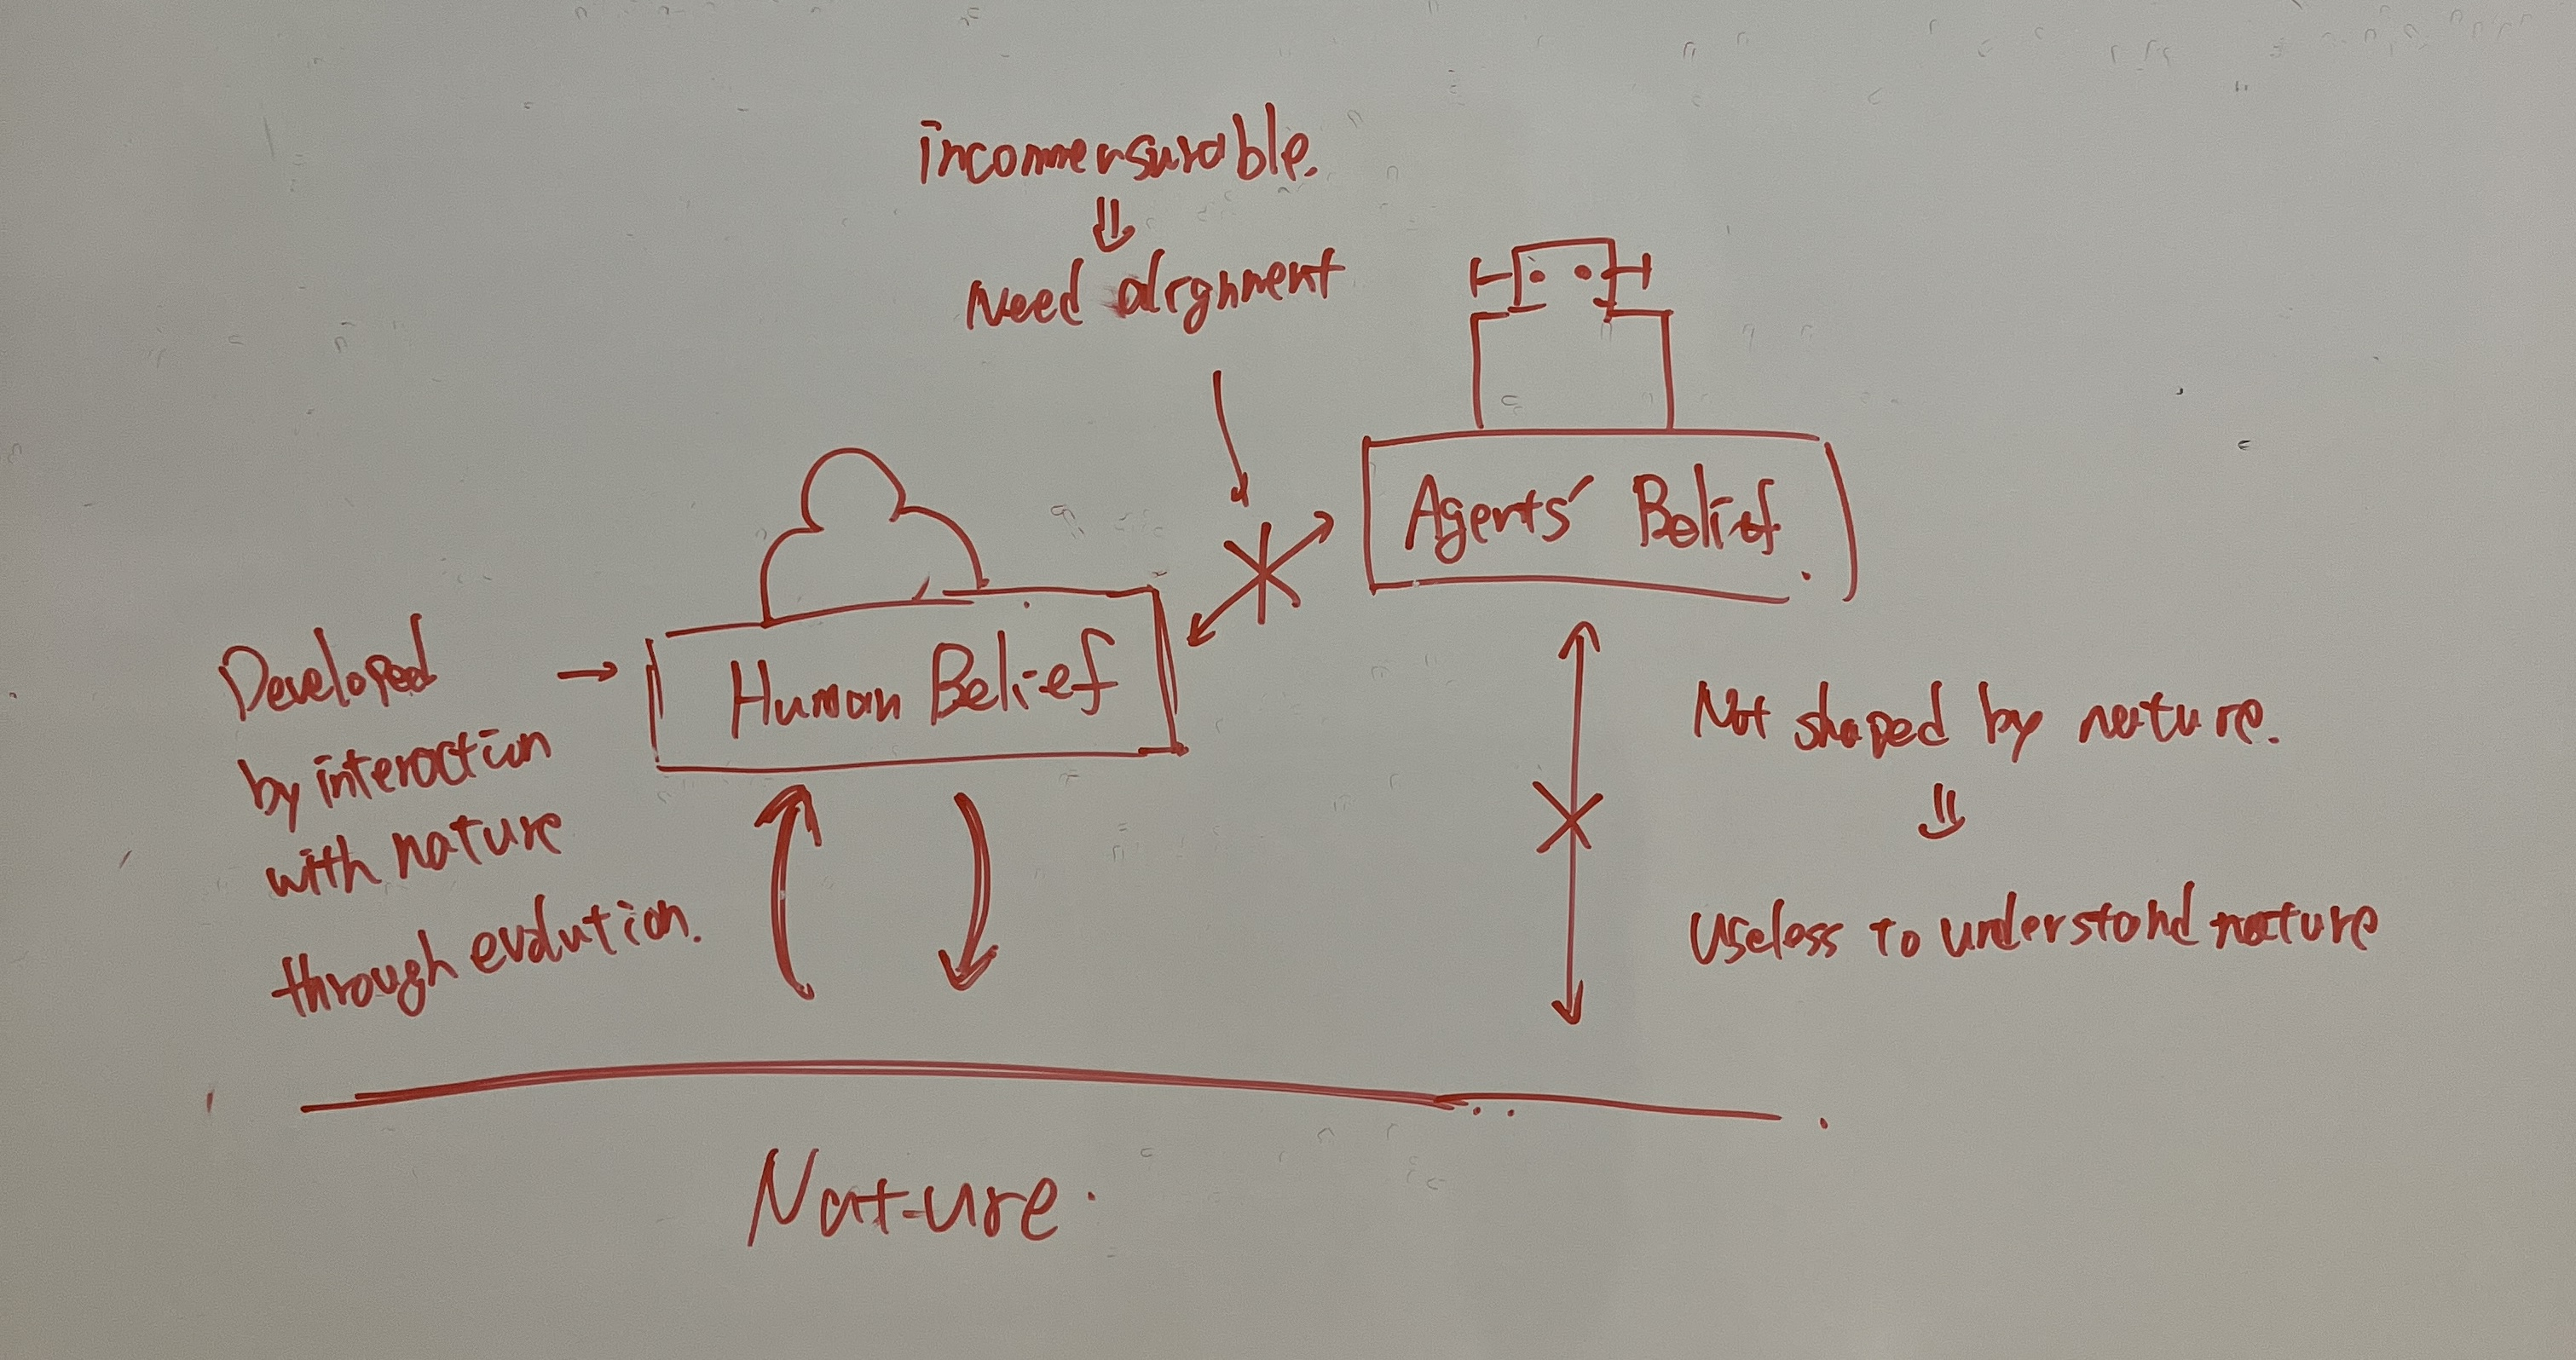
\includegraphics[width=\linewidth]{figs/incommensurability.jpg}
    \caption{Incommensurability}
    \label{fig:incommensurability}
\end{figure}

This all arises due to the expansion of the definition of research to include non-humans. Consequently, it is possible to aim for a definition of research strictly limited to knowledge production for the human society, and to ensure that artificial researchers exclusively engage in research for the benefit of humans. This appears to be more of a decision-making issue about what kind of future we want to pursue, rather than determining which definition of research is correct. Alternatively, it might be worth reconsidering the definition of knowledge production as the mere updating of beliefs. Engaging in discussions about this problem seems to be of great importance for the future of human society.

% First, knowledge is based on beliefs, so if a non-human agent holds beliefs, it would be reasonable to consider that they possess knowledge, even if they may not resemble human knowledge on the surface. The nature of beliefs is a complex matter to define concretely. However, even in current machine learning, models have confidence levels and prediction errors, which we believe are not completely unrelated to what we consider beliefs. Furthermore, even if the knowledge is not understandable to humans, if it is understood among a group of agents, meaning it is reduced to a shared belief, then it can be called ``knowledge for that group of agents.'' If a group of agents has means to update a belief to such a strong shared belief, then we consider it as research. From these reasons, we believe that research is conceivable for entities other than humans. And it feels like this is a highly significant conclusion in terms of contemplating the development of intelligent systems capable of conducting research.

% \textcolor{red}{TODO: Add relations with relativisim, maybe added to alignment section?}
% This position may have some similarities with a famous stance in philosophy of science that argues everything is, at its core, subjective, relative or a matter of belief \cite{chalmers2013thing,kuhn1962,howson2006scientific}. However, what we want to emphasize here is that we think the characteristic of research lies in tying beliefs about an object to stronger beliefs. And we believe that it is this strength of conviction, which seems self-evident to many people, that lends objectivity and persuasiveness to the claims of science.

% This is not definition but practically we think that one characteristics of research is its rigor of confirmation method. Firstly, you may wonder if anything unknown would suffice. We believe that research does not choose its subject and anything unknown is acceptable. Rather, what's important is the strictness of the methodology – whether the unknown truly became closer to the known, whether it was concluded into a stronger belief. Generally, the method employed by what we call research is designed with extreme precision, and as a result, it seems to withstand rigorous evaluations. This can be considered a major feature that distinguishes research from other various activities.

\subsection{Interim Summary}
In this section, we have discussed a provisional working definition of research. We started with the naive intuition that research is the endeavor to generate new knowledge for a society. We then explained that knowledge is belief, the production of knowledge involves updating beliefs, and the produced knowledge needs to be novel and supported by the common strong beliefs of a community. Lastly, we discussed based on these conclusions the possibility of research conducted by agents other than humans.

Reflecting on what research entails is highly important as it provides clarity on what we should truly strive for and offers guiding principles for our efforts. The discussion in this chapter suggests us that we need to discuss how to instill these abilities to artificial intelligence so that we realize a general artificial researcher to understand this universe.

The definition discussed here is merely a provisional one based on the naive perspective. By combining insights from philosophers of science, epistemology, and all working researchers, we can engage in a deeper analysis of the denfintion of research to develop more fruitful and reliable guidelines for our goal.

% The reason we deliberately distinguished between mere knowledge and knowledge for humanity is because we believe that there could be knowledge for beings other than humans. As we have repeated, understanding is subjective, so if machines start conducting research in the future, it is natural to think that there will be unknowns for machines and beliefs for machines. Therefore, it's possible that we could live in a world where humans produce knowledge for humans, machines produce knowledge for machines, we could live in a world where knowledge is produced for all agents including machines and humans, or we could continue living in a world where knowledge is produced solely for humans. In this sense, we believe one of the problems that will be questioned in the future is whose objectivity and whose belief we are talking about. We will discuss this point in more detail later.

%%%%%%%%%%%%%%%%%%%%%%%%%%%%%%%%%%%%%

% When a hypothesis survives a test, it was said that our belief in the likelihood of the hypothesis strengthens. Empirical science implicitly assumes a principle that relies on inductive reasoning as the basis for these tests. For example, we believe that if the number of observations consistent with a certain claim increases, that claim is more likely to be valid (this is called the principle of confirmation). Additionally, we hold the belief that unless other factors change, what has held true so far will continue to hold true (this is called the principle of uniformity of nature). These principles of confirmation and uniformity are the foundations of inductive reasoning, and they are unavoidable in empirical science. However, both the principle of confirmation and the principle of uniformity are merely beliefs, and there is no guarantee anywhere that these are ``correct''. The reason these can serve as the foundation for testing is because these beliefs are far more solid than the belief in the likelihood of a hypothesis that someone has just recently presented. That is, empirical science could be described as an endeavor to update the likelihood of a hypothesis by tying the belief held about a certain hypothesis to a more solid belief. While mathematics and logic are rare examples, considering that all other research endeavors are fundamentally empirical, \textbf{it may be possible to rephrase the endeavor of research, that is, the production of knowledge, as largely an endeavor to update our belief in the correctness of a certain object.} In fact, it is widely accepted in philosophy that knowledge requires belief \cite{sep-epistemology}. More formally, it's believed that "\textit{the three conditions—truth, belief, and justification—are individually necessary}" for knowing a fact \cite{sep-epistemology}.


% \subsection{Disclaimer Regarding the Characteristics of Research}
% we have mentioned that research is an endeavor to transform the unknown into the known, but you may question what distinguishes it from other activities that appear to do the saus. This issue arises from the fact that we have not properly defined knowledge in this paper. In this paper, we won't discuss this in detail but will limit myself to a brief disclaimer.


% \subsection{The Previous Discussions Regarding the Definition of Research (Scientific Discovery).}

\section{Knowledge Production System}

% \textcolor{red}{TODO: more focus on the implication for research automation}

% It is believed that research began with individual and concrete tasks. Among them, common actions were patterned and crystallized as a scientific method. We currently recognize this abstract set of behaviors as research. For example, hypothetico-deductive method and hypothesis testing are abstracted scientific method.

% Also, researchers use a research paper as a medium of knowledge transfer. Therefore, there are patterned activities related to a research paper. Examples of these include conducting surveys, gathering information from papers, and writing a thesis.

% Note that these are necessary tasks just because we use a paper as a medium of knowledge transfer, but they may not necessarily be indispensable for generating new knowledge. There are other such tasks as well. For example, peer review and fund raising are essential to current research practices in society, but they may not necessarily be indispensable for knowledge production.

% In this way, various tasks arise in conjunction with research. When considering the automation and optimization of research, it is desirable to consider streamlining all of these tasks. However, in this article, we focus on the process from determining a research topic to publishing a research paper. We will refer to this process simply as the \textit{research process} from here on.

% \subsection{Overview}

% As mentioned earlier, research is an attempt to turn the unknown into the known. Therefore, the research process can be seen as a function that takes the unknown as input and outputs the known. However, in reality, a single research paper may not be enough to turn the unknown into the known. Therefore, in practice, the research process is considered to be a procedure that takes the unknown as input, and outputs a text that describes the procedures and their results, as well as their interpretation, in order to turn the unknown into the known.

% First, let us structure the common research process. In particular, we will base the structuring of the research process on the method of empirical science, which many researches rely on as a foundation. However, we believe that this framework can be applied to other research activities, such as mathematics, as well. We will explain the reason for this later.

% The research process, especially that of empirical science, is carried out through the following steps: topic decision, hypothesis generation, verification design, verification, and analysis of experimental results. The outputs of these steps are then written into a paper, which undergoes peer review and is eventually published.

% Note that some commonly seen items, such as surveys, are not included here for a reason. First, as mentioned earlier, gathering information from papers is only a means of knowledge transfer through the use of a thesis. Second, information extraction from papers can be done at any stage of the research process. Thus, we believe that processing related to a paper, such as \textit{reading papers} and \textit{writing a paper}, needs to be considered separately from the aforementioned research process.

\subsection{Overview}

% \textcolor{red}{TODO: reconsider the research process, structure of knowledge production system, and the scope of this paper}

The definition of research stated in the previous chapter is somewhat too abstract to serve as a concrete guideline for building something based on it. Moreover, it feels distant from the research practices employed by humans, making it challenging to immediately connect our standing point to with the goal. While the ultimate goal is to achieve a fully end-to-end system for conducting research, it is practical and useful to start by discussing how to realize individual sub-processes within the research process. Breaking down the research process into partial processes will make the functions that need to be achieved much clearer.

Therefore, we attempt to structure the research process a bit more by decomposing it into its constituting elements. Specifically, we will divide the process of producing knowledge from any given input into appropriate sub-processes. During this division, each sub-process will be structured with the level of abstraction required for all types of research. This is because the aim of this paper is to achieve a general artificial researcher. Hence, even if an element seems crucial in current research, if it is not necessarily essential to the definition of research seen so far, we will treat those elements separately from the constituents of the research process in this study. By separating these elements, we intend to clarify the indispensable components for realizing an artificial researcher. 

% \subsubsecti on{Outline of the Structure}
% In this section, we will discuss the three things tightly related to the knowledge production. We will first discuss the functionally essential elements for knowledge production system, which is the abstract structure of the research process that has been emphasized so far. These elements correspond to the modules in knowledge production system. This is a main topic of this chapter. 

% For convenience, we will refer to the entire structured research process as the \textit{knowledge production system} or just \textit{research process} throughout the rest of this paper.

% In the previous chapter, we discussed the definition of research. In this chapter, we will focus on the high-level abstract structuring of the research process while paying attention to its functional aspects. By emphasizing the functional aspects, we mean paying attention to the role that each step plays in knowledge production. By higher-level abstract structuring, we intend to focus on the processes that is as universal as possible across research fields, regardless of the specific domain. The purpose of this kind of structuring is to clarify what kind of modules should be created as intermediate steps of research when aiming for research automation. In the following, we will structurize the research process into a chronological sequence for the purpose of clarity. However, it is important to note that the focus lies not on the temporal order nor human convention, but rather on the functionality in relation to knowledge production and the inputs and outputs of each of these processes. Also, as previously mentioned, because humans are currently the primary knowledge generators, there are many constraints that come from human society. Thus we will do our best to distinguish and organize what is dependent on humans and what is not. Before delving into specific discussions, let us first explain the scope of this chapter. After that, we will discuss the outline to be addressed in this section, followed by the main discussions.

\subsubsection{Scope of the Discussion}
We think that the activities related to research can be broadly divided into two phases: the process of knowledge production, typically in the form of papers or other publications, and the phase of maintaining, sharing, evaluating, and utilizing the knowledge. While the latter phase is a crucial aspect of knowledge, it will not be extensively addressed here since our interest primarily likes on knowledge production. However, it's important to note that the distinction between the two phases is not strictly delineated. For instance, how knowledge is used often influences the production process. Additionally, research evaluation and revision are ongoing processes, and as mentioned earlier, belief updates are not set in stone. Thus, evaluation of the value of knowledge may not be completely exclude from our discussion simply because they mainly take place after knowledge production. As such, given the difficulty in making a strict demarcation, we will make sure to touch upon elements that are not necessarily considered for knowledge production even within the latter. The aforementioned distinction is merely a matter of emphasis, and it should be understood that it does not imply completely disregarding the latter phase.

Furthermore, factors influenced by social constraints such as funding acquisition and collaboration agreements that typically occur before the research are not addressed in this paper. Knowledge production can be seen as a function that produces knowledge from inputs such as people, capital, resources, and information. Viewing it this way, the acquisition of money or human capital can be considered inputs to the function rather than the knowledge production itself. Thus, we do not touch on this topic in this chapter. We admit that these factors are also crucial elements in the pursuit of true autonomy in research, so they will be subject to future discussions. Also, even if it is information acquisition, if that is strongly related to the internal of knowledge production itself, we will address it later in this paper. 

In conclusion, the following text focuses on the process of research, where knowledge is output as research outcomes given any input. For simplicity, we will refer to this process as the \textit{knowledge production system} or just \textit{research process}. It is worth reiterating that this distinction is provisional, intended to facilitate further discussion and the development of better categorizations or broader automation in the future.

\begin{figure}[htb]
    \centering
    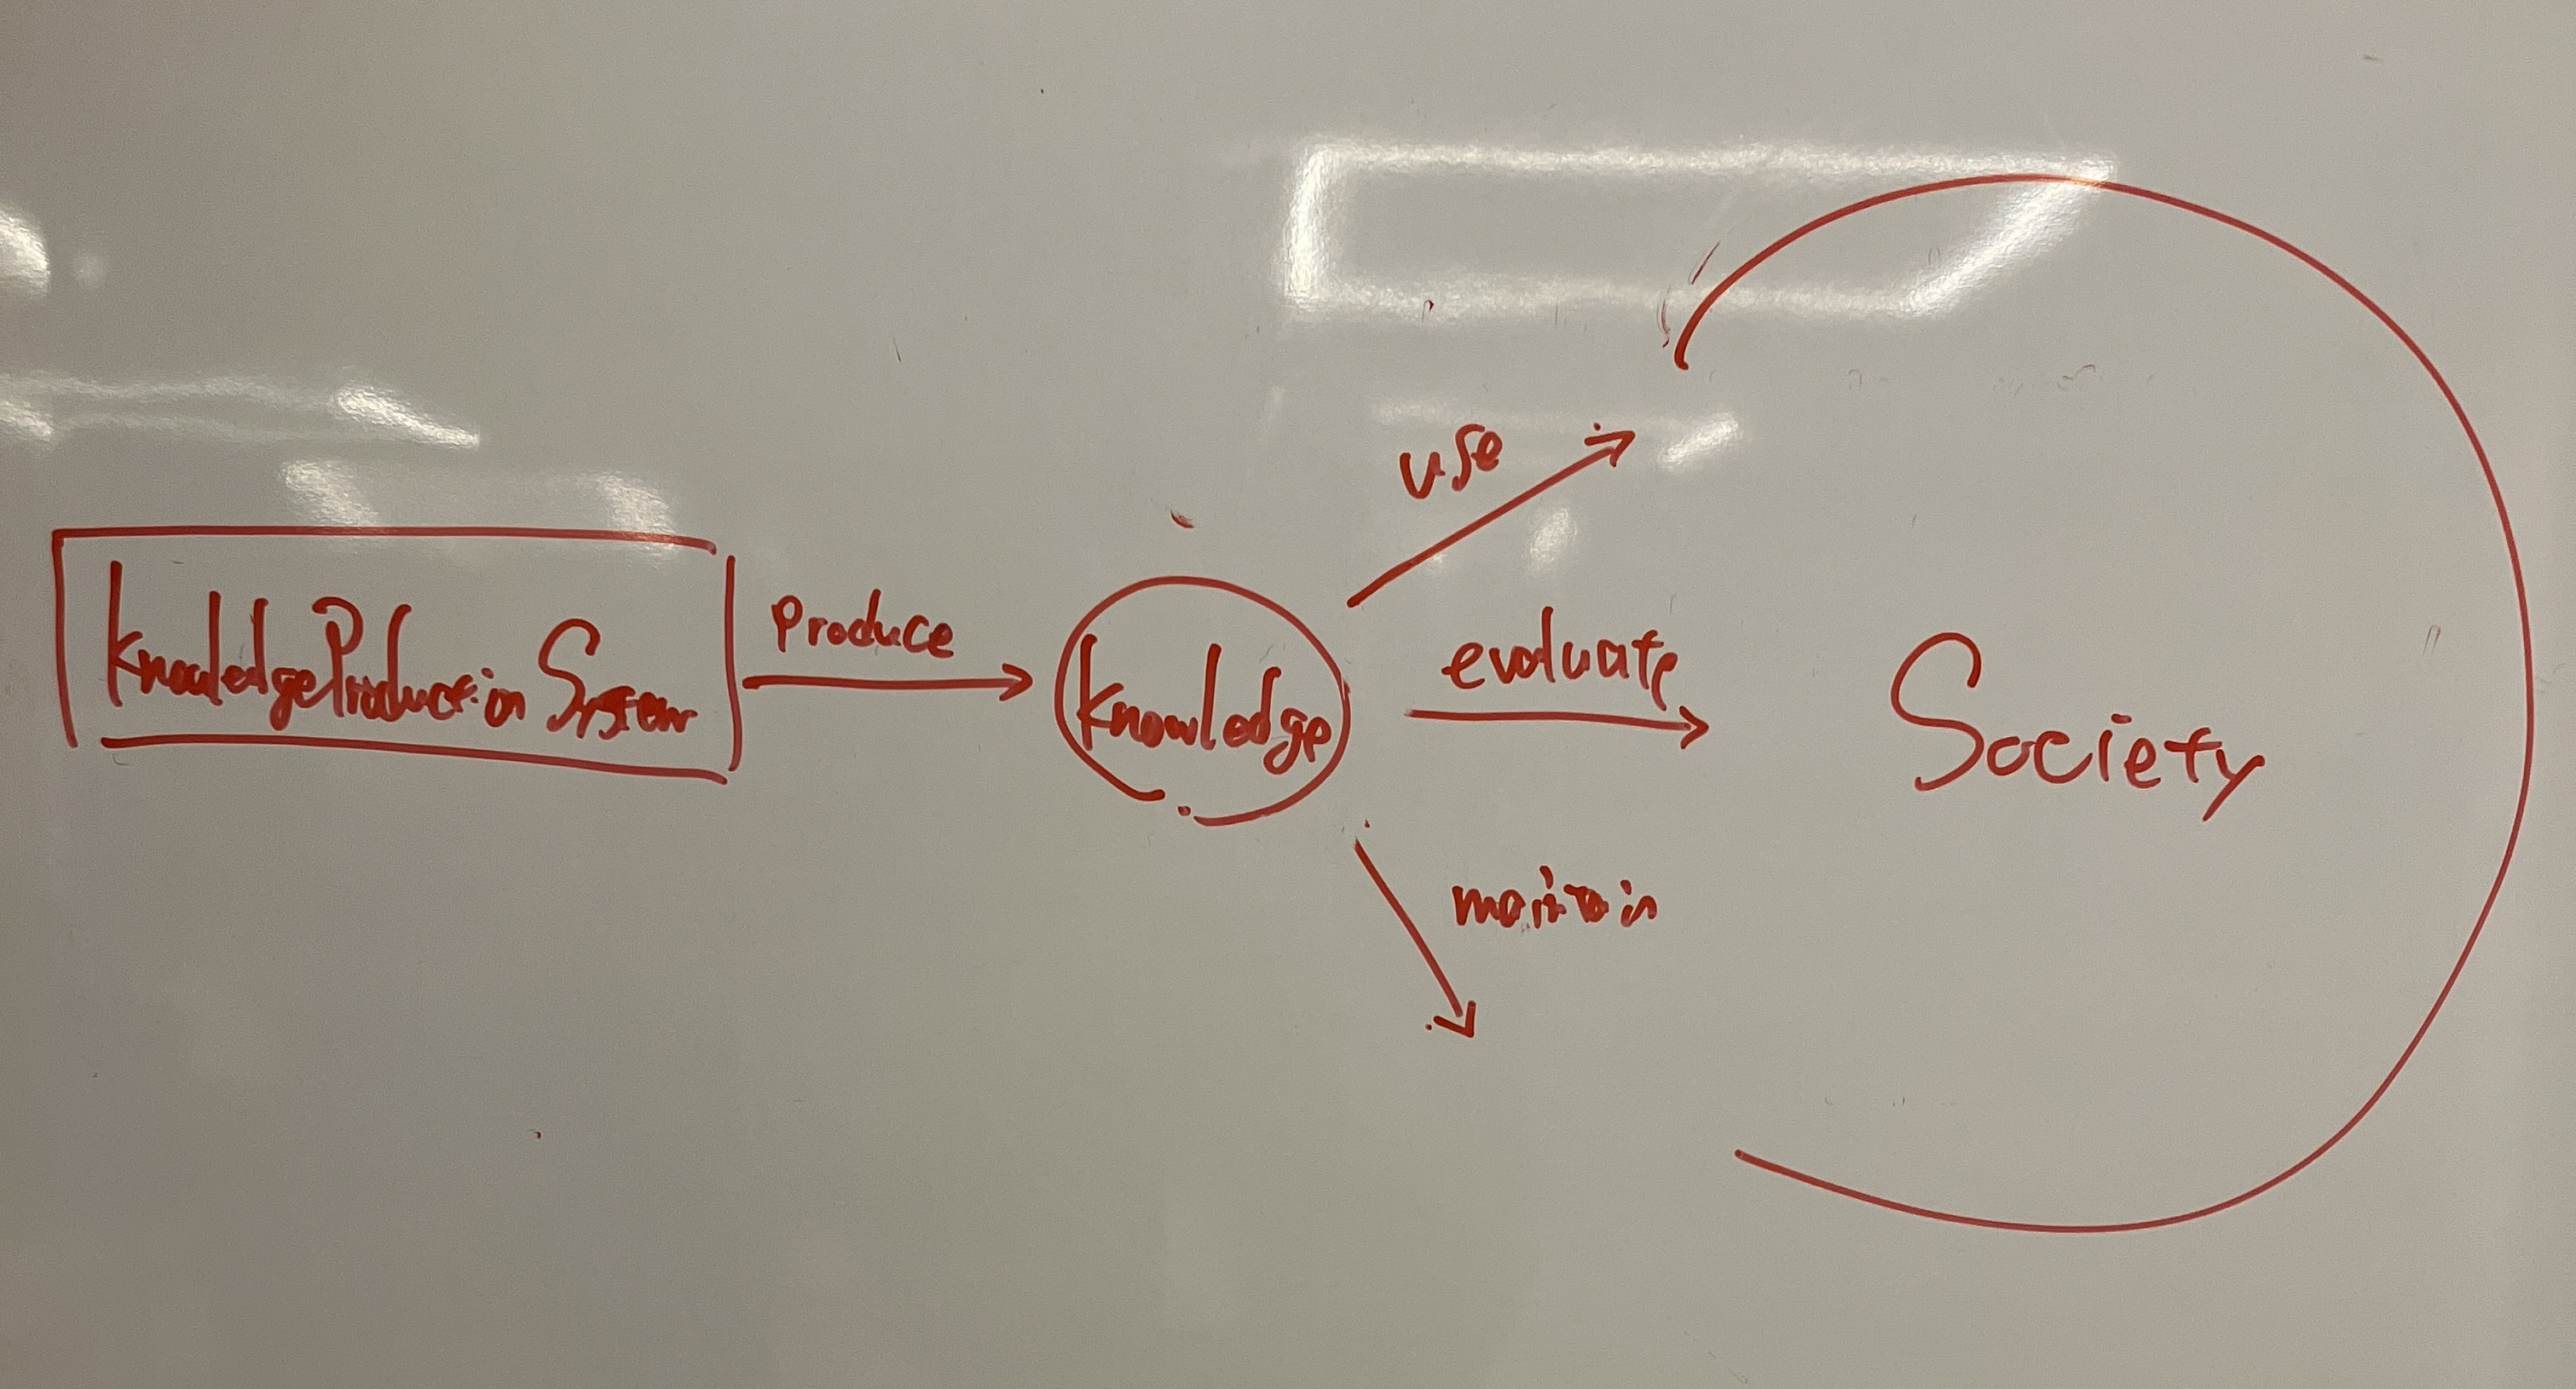
\includegraphics[width=\linewidth]{figs/research_process_society.jpg}
    \caption{Knowledge Production System and Society}
    \label{fig:research_process_society}
\end{figure}

% \textcolor{red}{TODO: add the excuse that research is social activity}



% \begin{figure}[htb]
%     \centering
%     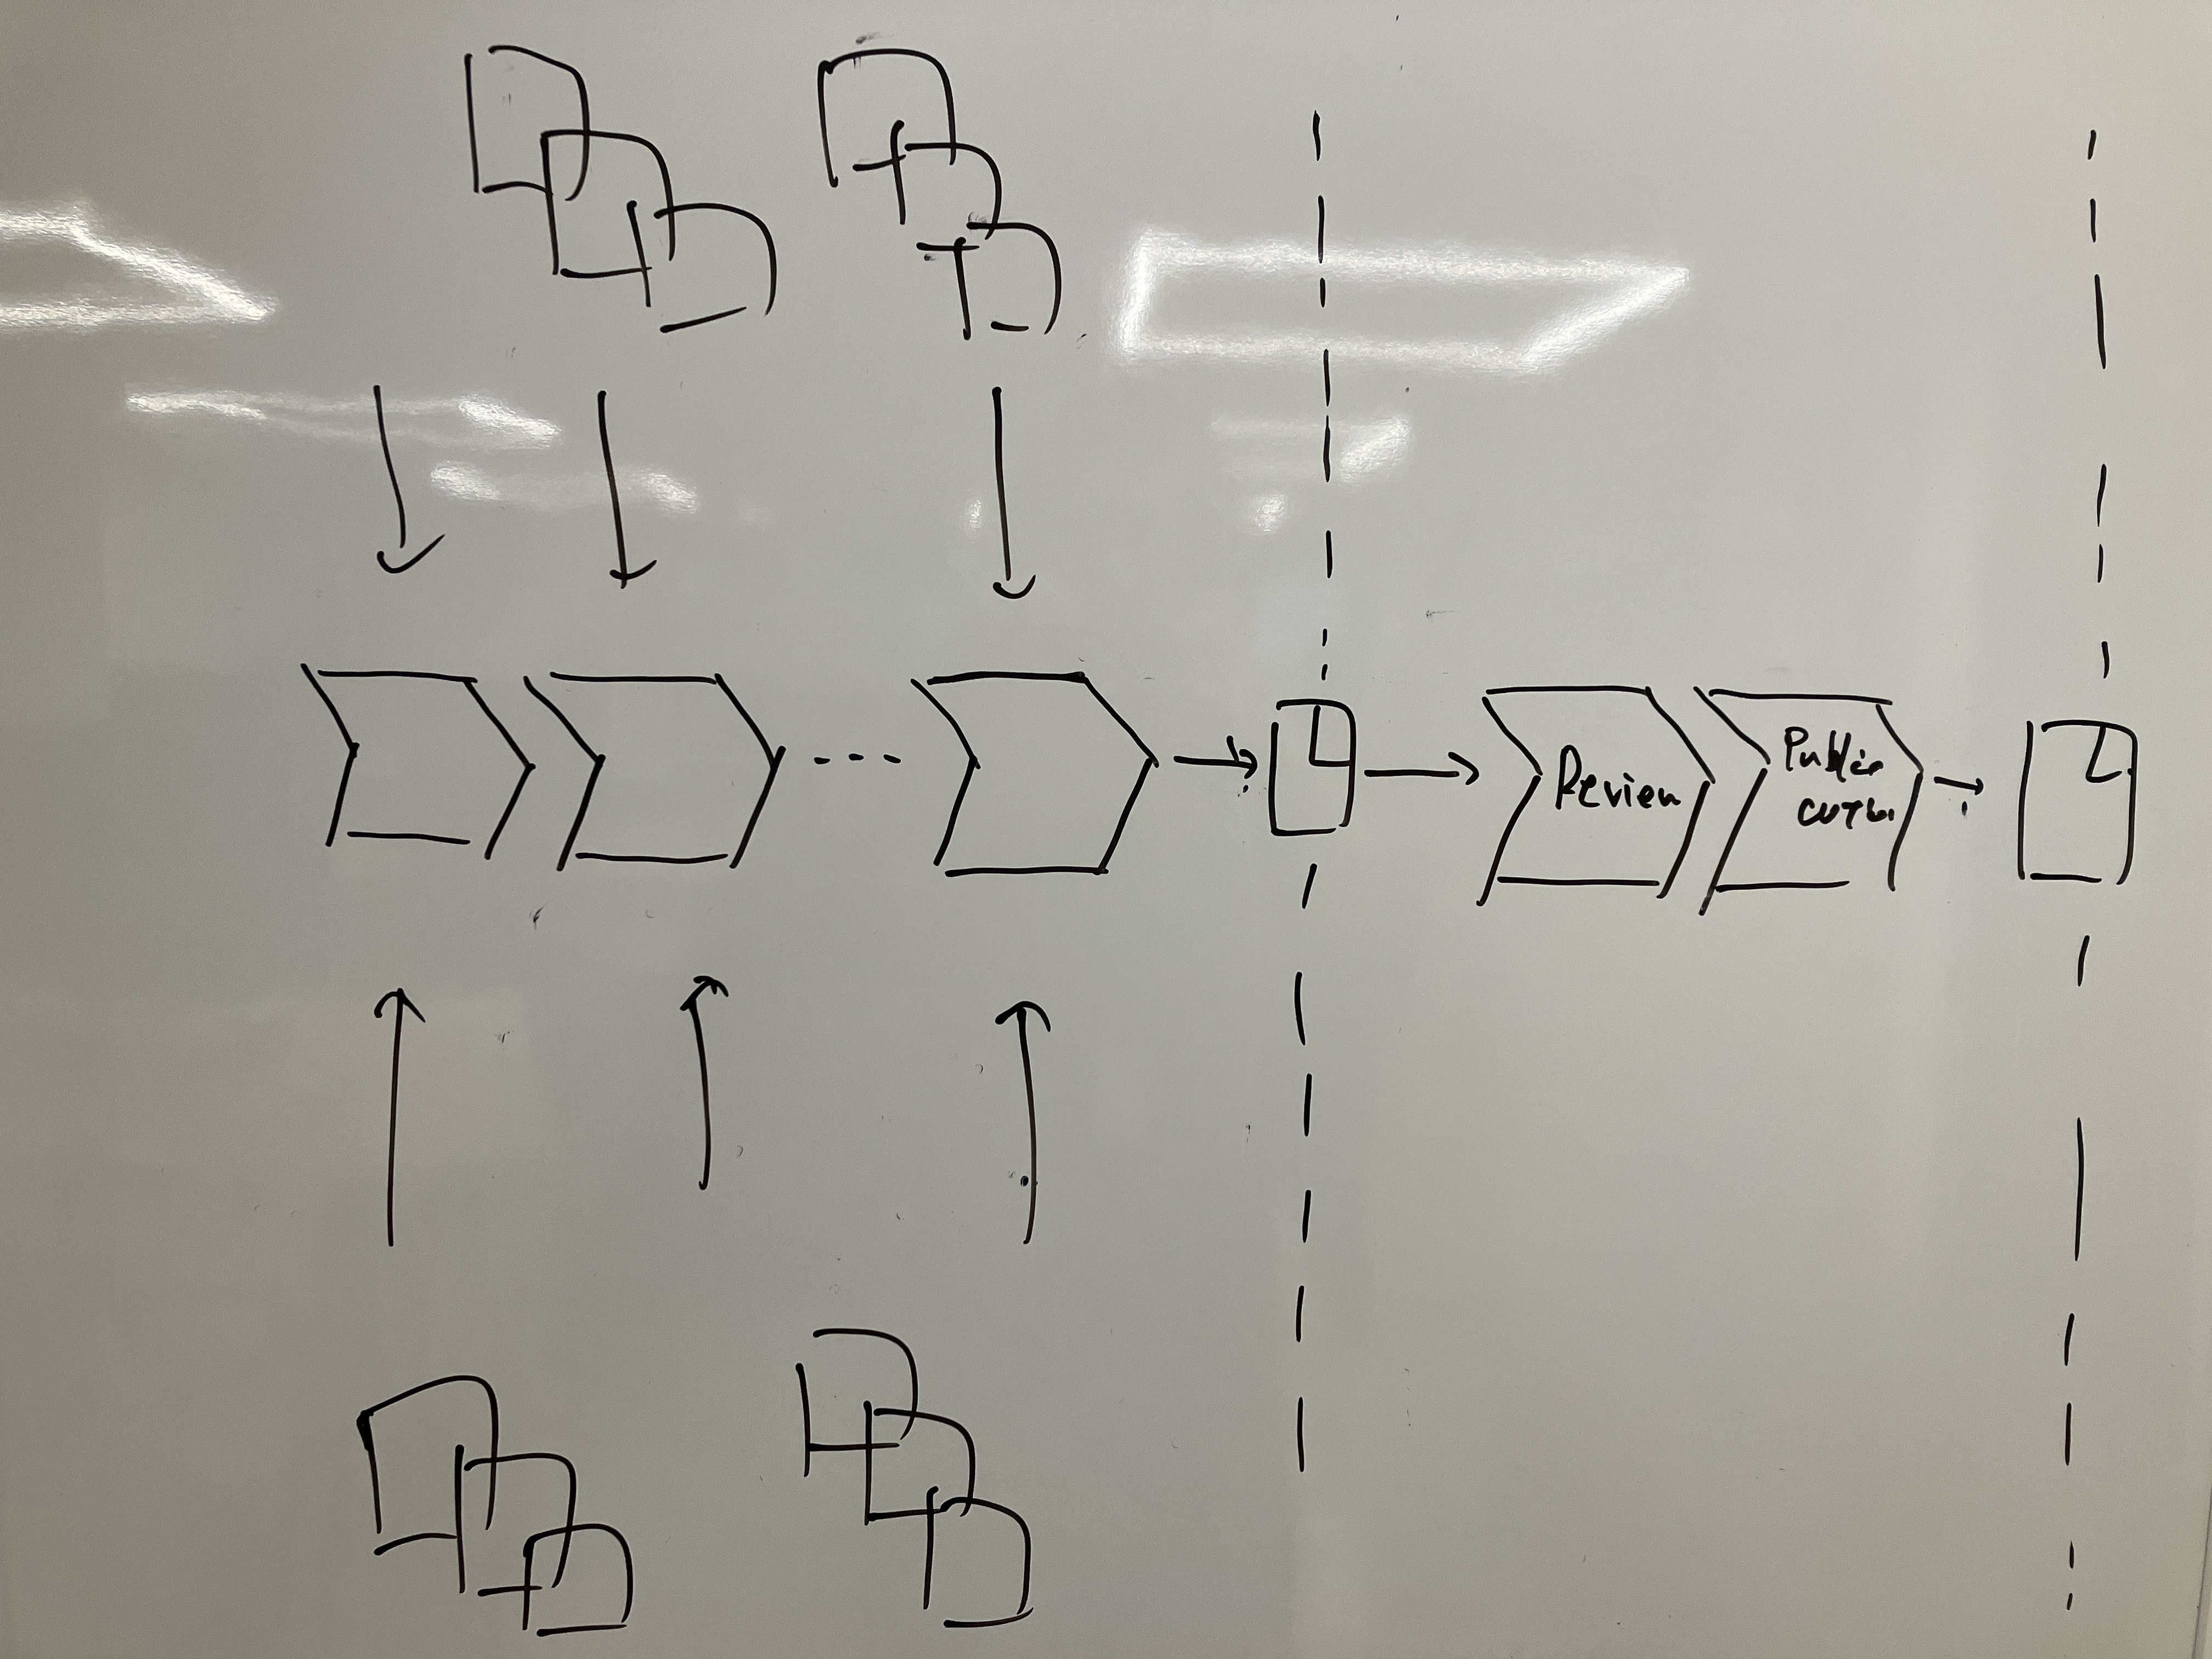
\includegraphics[width=\textwidth]{figs/researchprocess.jpg}
%     \caption{Caption}
%     \label{fig:research_process}
% \end{figure}


% Next, we will discuss a high level description of how human beings have been conducting research. I'll structurize the abstract pattern of the process (which we will call\textit{ research process}) from determining the unknown to it turning into known. 


% \subsubsection{Note}

% note, direction
% Though our structuring may seem to represent scientific methods, we believe this pattern cam apply to other research fields, such as mathematics and humanities as well. When describing the structure, we will make a conscious effort to clearly distinguish between essential elements for knowledge production and those that are not. As previously mentioned, because humans are currently the primary knowledge generators, there are many constraints that come from human society. When considering the possibility of machines conducting research in the future, it will be important to distinguish and organize what is dependent on humans and what is not.

% we believe that the conduct of human research activities can be roughly divided into three stages: knowledge production, knowledge evaluation, and knowledge sharing. 

% Although these may not necessarily be distinctly separable from each other, we adopt this classification because it is useful for advancing discussion. The process of knowledge production consists largely of the steps: problem determination, hypothesis generation, and hypothesis verification. And in this process, the ability to read and write documents and analyze data are required as necessary skills. Below, we will examine each of these in more detail. 


% This structuring is tentative and there may be a better way to structure the research process. However, we have created this structure for practical purposes in order to move the discussion forward. We hope the structure of this article be a starting point for conceiving a better structurization. We believe that structuring and deepening understanding of the elements that are essentially important for knowledge production is extremely crucial when aiming for the automation of research.

% Though we explained that research is belied revision, it would be convenient to see as a function that takes the unknown as input and outputs the known.  % TODO: rearrange

\subsubsection{Three Sub-Systems in Knowledge Production System}
In the following sections, we will explain three essential elements that we think are functionally necessary in knowledge production: \textit{question construction}, \textit{hypothesis generation}, and \textit{hypothesis verification}. These are the abstract structure of the research process that has been emphasized so far.

Constructing questions is equal to deciding the unknown to be investigated, which is necessary by definition for research, which is the art of bringing the unknown closer to the known. Generating hypotheses is inevitable when dealing with the unknown, although they may be implicit and the extent may vary. This is because if we did not require any inference with uncertainty, the unknown would not have been unknown in the first place. In other words, when dealing with the truly unknown, one must generate some hypothesis. The third element is hypothesis verification, which is a process that shows us how probable it is that a hypothesis is true. This element is indispensable, as it is converting our unjustified beliefs that a hypothesis is true into knowledge.\footnote{
While the term ``verification'' is used here, it does not imply a definitive determination of the truth or falsehood of propositions, as commonly used in philosophy. It is used in the sense of just strengthening beliefs as used in everyday language. Thus, ``confirmation'' may be a more accurate term, but verification is more widely recognized, so we will use that.
}

When summarizing these intermediate steps, it goes as follows: First, upon receiving any input, we formulate a question. Taking this question as input, hypotheses are generated. Finally, these hypotheses are input and validated resulting in the creation of knowledge as a research outcome. These processes are considered a proper decomposition of the research process, as they request each other's outputs as inputs and seamlessly connect the entire research process from input to output without any gaps.
% \textcolor{red}{TODO: However, we can identify discovery with justification because both are belief updates. I'll add this point wherever in this paper.} Fig. \ref{fig:knowledge_production_system}.

% \textcolor{red}{TODO: Add fig like this. add this sentence to the explanation of the fig "we approach the unknown to the known by asking questions, providing tentative answers to them, and then verifying the validity of those answers. " }.
% Fig. \ref{fig:research_process}.

\begin{figure}[htb]
    \centering
    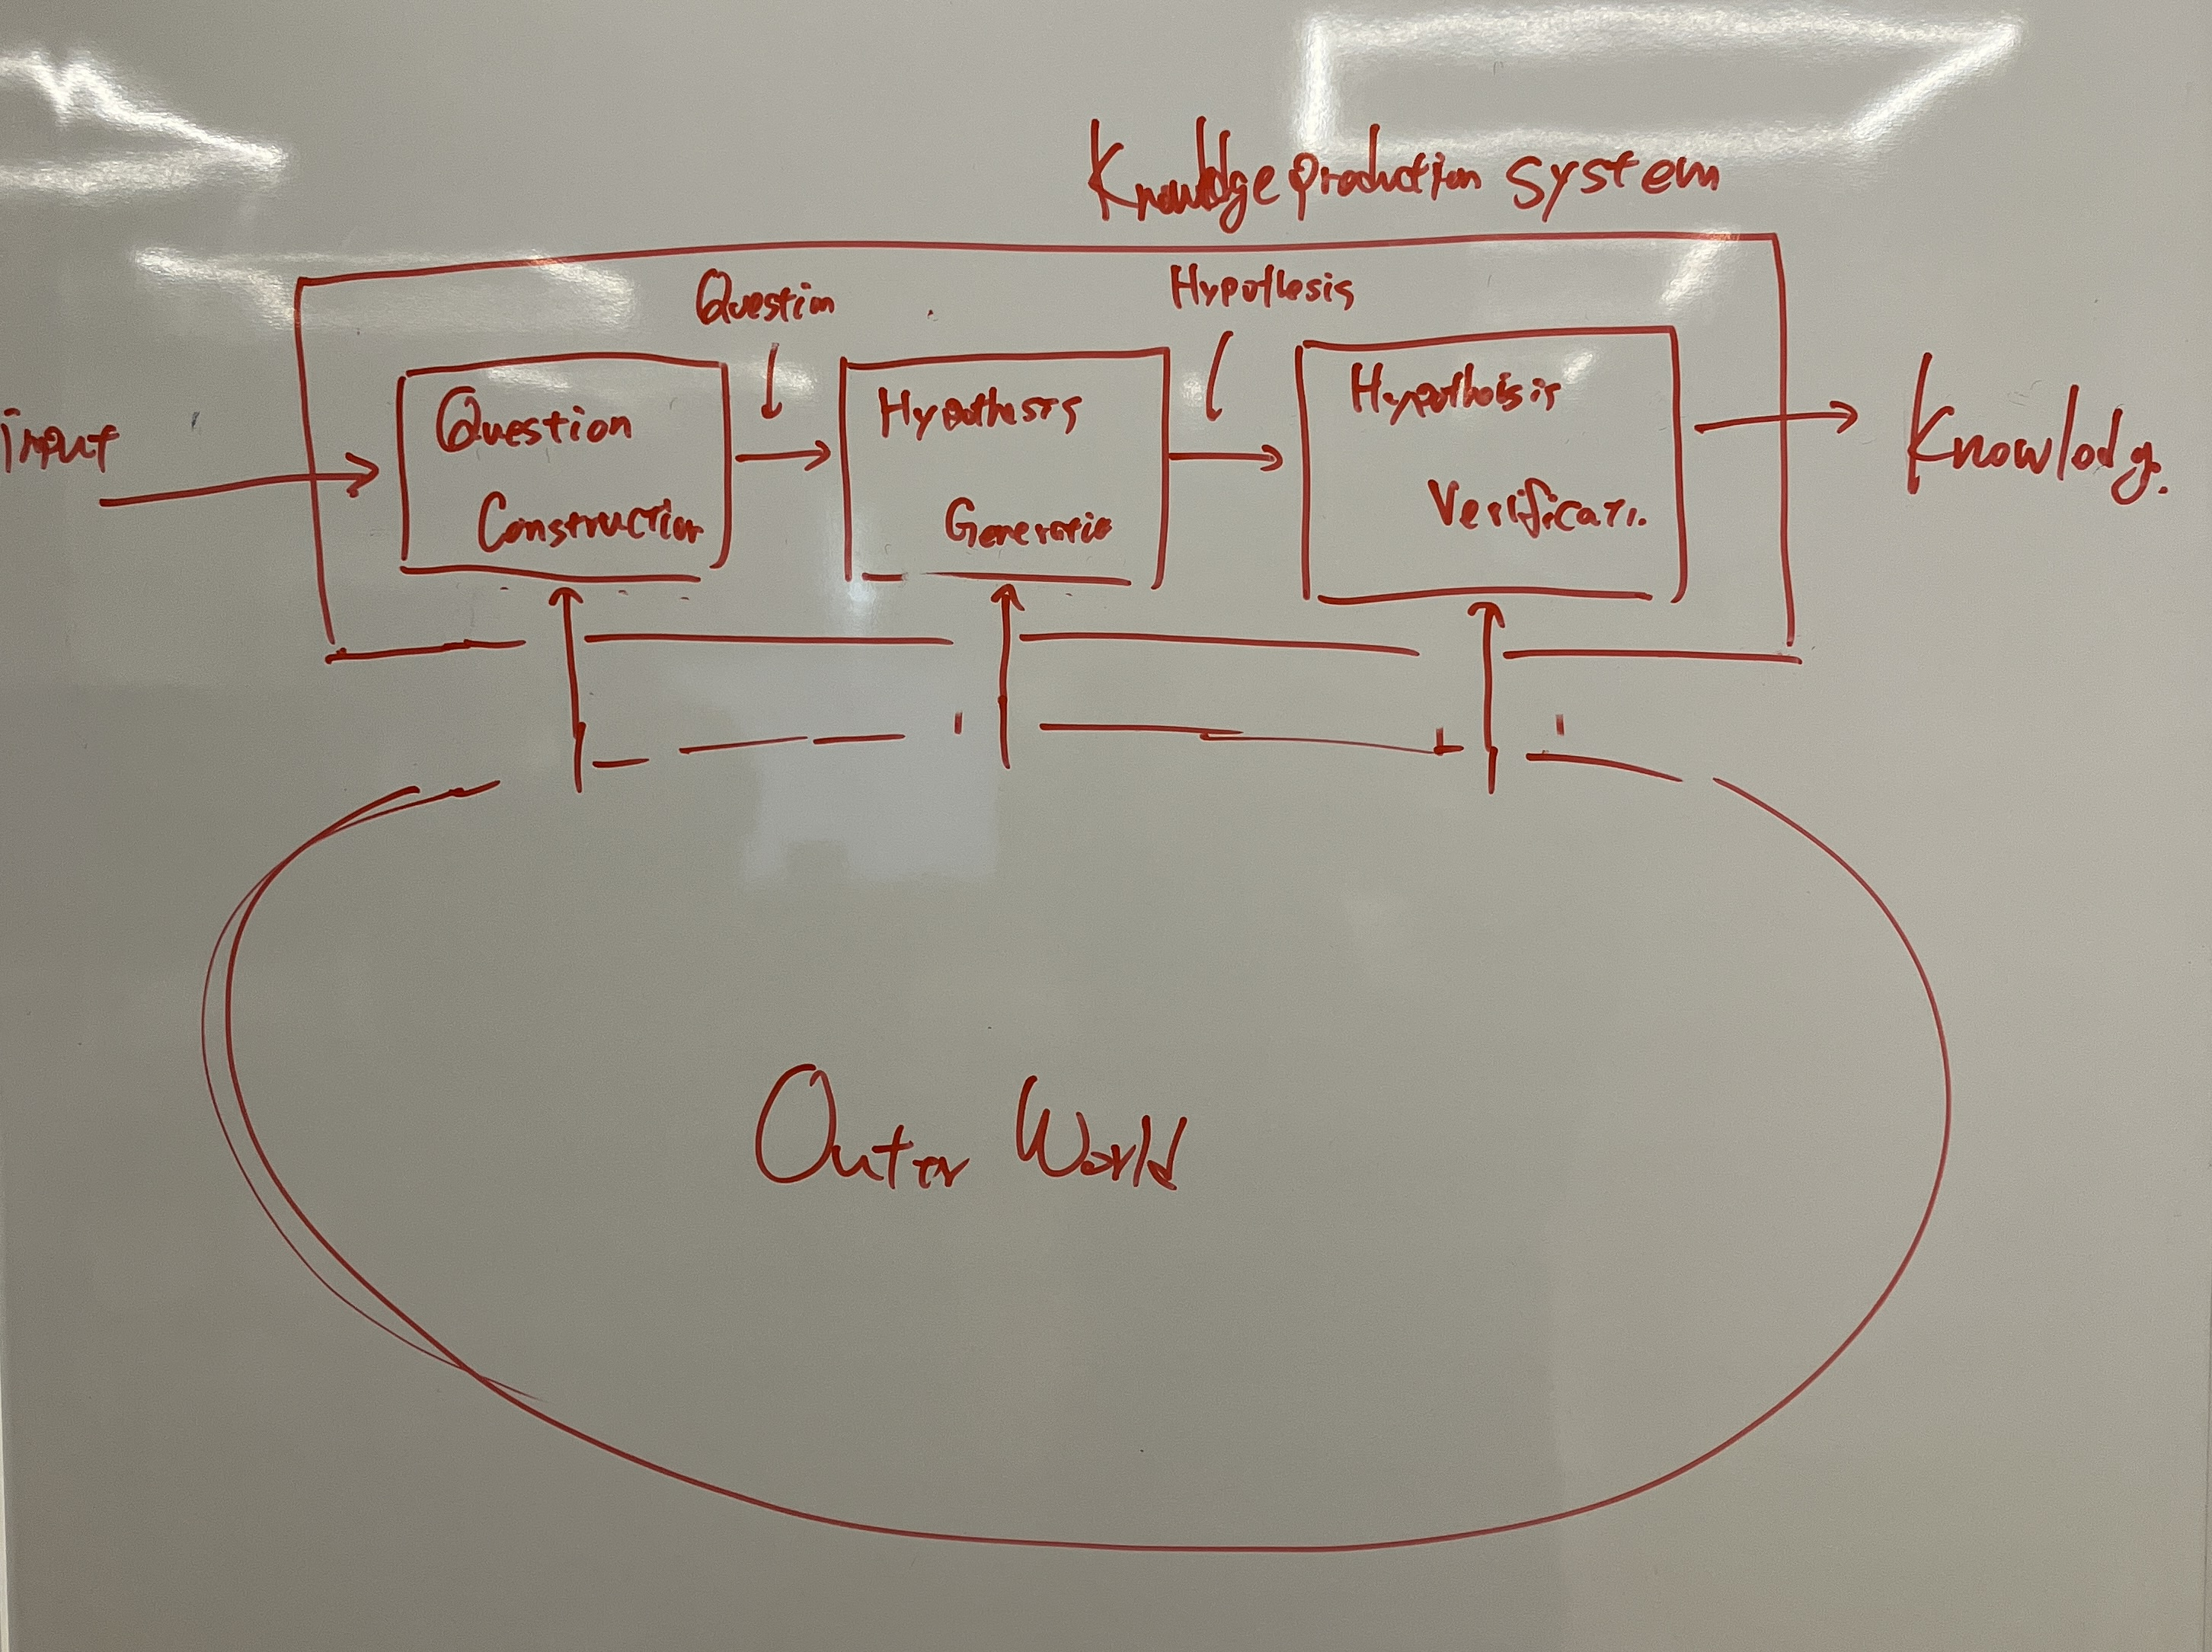
\includegraphics[width=\linewidth]{figs/knowledge_production_system.jpg}
    \caption{Knowledge Production System}
    \label{fig:knowledge_production_system}
\end{figure}


\subsubsection{Research as Information Processing System}
Our structurization so far is based on the perspective that research, in other words, the knowledge production system, can be seen as an information processing system.\footnote{Although our discussion here is influenced by David Marr's three levels  \cite{marr2010vision}, it is not exactly the same, so we mention it only in this footnote to avoid misunderstandings} First of all, all information procesing systems have an objective and achieve that objective by processing inputs. In our case, the objective in research is to produce a new knowledge for a society. The reason I divided the research process into the question construction, hypothesis generation, and hypothesis verification is equivalent to breaking down this information processing into three sub-modules. Each of these three sub-modules is also an information processing system with its own objective. For example, the objective of the question construction module is to discover unknown knowledge.

When we have mention in this section that we would focus on the parts functionally related to knowledge production, it have meant two things. The first is to ensure that the objectives of these sub-modules are essential sub-objectives in all research. As mentioned earlier, these modules should not be something that works for history research but not for mathematics research. We should consider modules that have objective essential to all research for realizing general artificial researcher. Additionally, the process of peer review, while relevant to knowledge production, was considered to be a process of judging the ``value of knowledge'' and so was not included in the knowledge production system. The second point is that the our discussion is limited to the objective of the modules and not about the specific representation of information or the specific algorithms for information processing within the modules. For example, reading and writing papers are currently universally necessary for any research. However, a paper is just one of all representations of information, and there could be alternative representations (e.g., blogs). Moreover, while one person may conduct experiments using rats to verify a hypothesis, another person may present historical records showing statements from deceased individuals that match the hypothesis. These are different methods of verification, but both serve the purpose of verification.

\textcolor{red}{TODO: Why this structurization is useful}

\begin{figure}[htb]
    \centering
    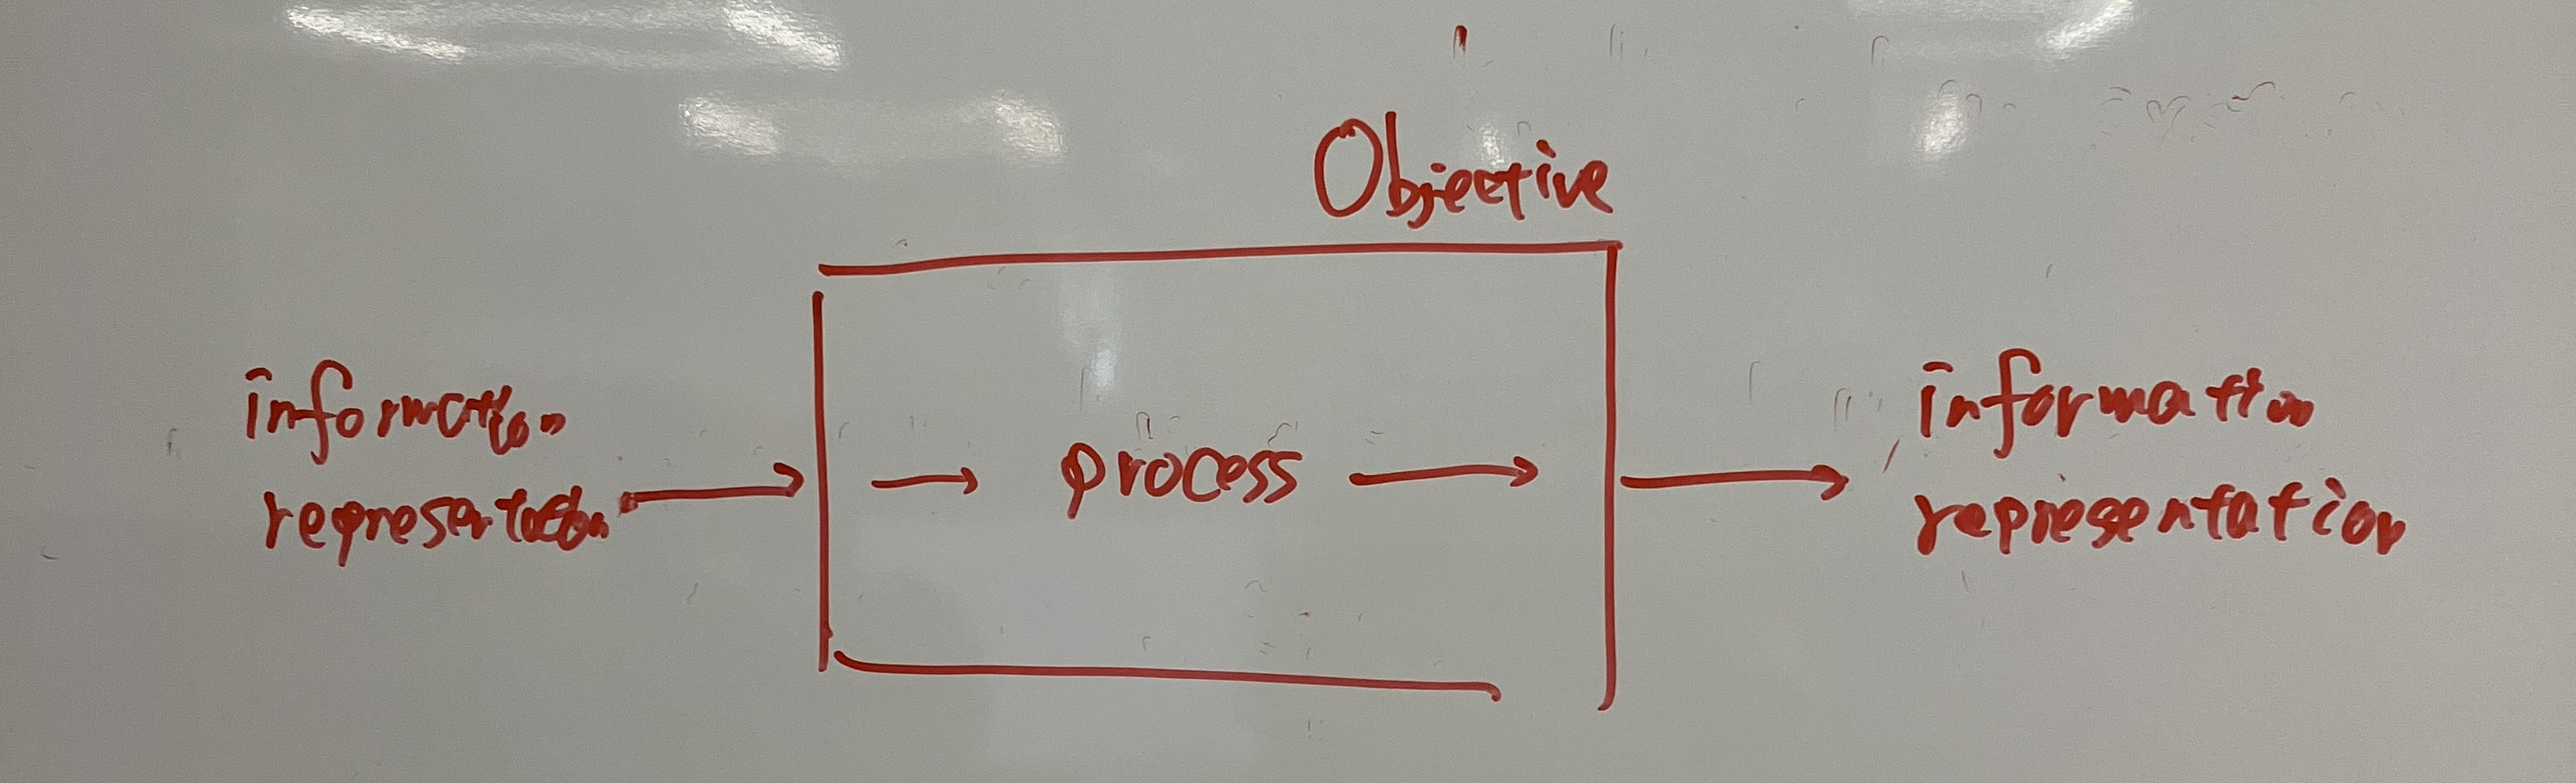
\includegraphics[width=\linewidth]{figs/information_processing_system.jpg}
    \caption{Knowledge Production System}
    \label{fig:information_processing_system}
\end{figure}

\section{Question Construction}
The first module of a knowledge production system should be question construction. This is because research is an act of generating new knowledge, and questioning is the act of seeking new knowledge. To initiate the process of generating new knowledge, one must first know what could potentially be new knowledge. In other words, we must know what we do not know. This is an essential function for research to be the production of new knowledge. And it is the task of question construction to fulfill this function. Therefore, question construction is an indispensable module in the knowledge production system.

Questioning is an act of seeking information \cite{watson2015ask}, which is knowledge in the case of research. The process involves two steps: 1. Recognizing missing information, and 2. Attempting to fill that gap. For example, the process of asking why the sky is blue starts as follows: when prompted by something we realize that we don't know why the sky is blue, and then, if we would like to know the answer, utter the question, ``Why is the sky blue?'' 

Here, we explained the process as first determining something as unknown and then deciding if you construct question about the unknown. However, the order doesn't matter. For instance, there may be knowledge that you want to know first, and then you confirm that it is indeed unknown. What matter is that, to create a module for question construction, it is necessary to consider how to achieve these abilities: recognizing missing information and deciding if you construct question. 

\subsection{Recognizing Unknown}
When prompted with a specific type of knowledge request and upon referencing our own knowledge, if we judge that we do not possess that knowledge, we recognize it as unknown to us. For example, let's say someone tries to explain why the sky is blue. ``Explanation'' calls for a type of knowledge, the ``reason'' behind why the sky is blue. When this person thinks about it and cannot provide an explanation, they recognize that they do not possess the knowledge of the ``reason'' why the sky is blue. Here, at least two things are happening. First, referencing one's own knowledge, and second, assessing whether there is expected knowledge.

\subsubsection{How Human Judge Unknownness}
In the case of humans, the process of recognizing such knowledge as unknown seems to involve retracing whether they have any "memories" of knowing, using, or hearing about that knowledge. When no relevant memories come to mind, the person may infer that they do not possess the knowledge. Even if the memory does not exist, they might try to use existing knowledge to answer the question. When they cannot construct a valid answer they are confident about, we consider it a recognition of not knowing. As mentioned earlier, to recognize a piece of knowledge as unknown means not having a justified belief that a proposition is true for a particular subject. Thus, the criterion for judging "being unable to construct a confident answer" can be seen as not having a justified belief.

While we have discussed recognizing unknowns for individuals, in research, what is essential is recognizing unknowns for society as a whole. If there is a way for an entity to identify societal unknowns without going through the process of identifying unknowns for individuals, that would be ideal. Therefore, we will discuss how to recognize societal unknowns.

Currently, the most widely used method for determining novelty is through literature surveys. Knowledge for humanity is primarily disseminated through research outcomes. Therefore, when examining all the research outcomes that have been generated thus far and finding that none of them provide an answer to a specific question, it seems reasonable to conclude that the question possesses sufficient uncertainty to warrant further investigation as a research endeavor. In particular, humanity has developed the culture to preserve the research outcomes in the form of papers. Therefore, it seems feasible to assess the unknown nature of an inquiry by examining all academic papers. There are various methods to determine whether the desired knowledge already exists. Typically, it is considered that candidates can be narrowed down in two steps. First, since research papers are composed of questions and their corresponding answers, one can search for papers that have similar questions and answers to the desired knowledge. Once these papers are found, the validity of their verification methods is evaluated.\footnote{
The discussion of assessing the validity of verification greatly overlaps with the content to be discussed in the chapter on hypothesis testing. Specifically, what's needed here is the evaluation of testing, whereas what's required for the automation of hypothesis testing is the generation of testing. In this sense, the latter discussion includes the discussion here. Therefore, we will refrain from discussing this here and touch on it later.
} If it is determined that sufficient verification has not been conducted, it can be concluded that the knowledge does not exist. 

It is impossible to review them all due to constraints in terms of time, technology, and cognitive limitations. Therefore, in practice, we consider a question as unknown if it has been sufficiently and comprehensively explored through an extensive examination of these academic papers. We conduct literature reviews to synthesize existing research, identify research gaps in existing studies, and thereby ascertain the unknowness of our own questions or construct question for which the answers are unknown \cite{schryen2015theory}. However, in reality, such rigorous literature research is not always conducted in every case. Instead, researchers judge the unknownness of the answer to the question by referencing only a few related works and explaining that none of them have yet resolved the unknown. This means that a subjective evaluation criterion is being used because of the limitation of the number of papers we can read. 

\subsubsection{Implication for Artificial Researcher}
So far, we have provided an overview of what it means to recognize unknowns and how it is currently being done. Now, let's discuss the implications if these processes were autonomously performed by machines.

The first possibility is an alternative to literature surveys. This situation involves the world's knowledge being stored discretely in units such as research papers, which is essentially the same method humans currently use to determine novelty. However, machines far surpass humans in terms of information processing capacity and speed, which could lead to significantly more efficient and statistically accurate determinations of novelty compared to humans. Since unknownness is a fundamental aspect of research, statistically rigorous judgement by machines would be desirable for the future of research.

% This current convention stems from the cognitive constraint that there is a limit to the literature that humans can examine. Since unknownness is a fundamental aspect of research, ideally, it should be evaluated objectively and rigorously. For instance, it would be desirable to quantitatively state which journals, what types of papers, and how many have been examined, and the result indicating their unknownness. Although systematic reviews already employ such approaches, there is, of course, a limit to the number of papers that can be evaluated manually and selection biases cannot be removed.

Considering that knowledge production by machines is likely to occur in the future, it may still be challenging to examine all knowledge exhaustively. Therefore, discussions on efficient search methods and how far one should investigate before determining novelty become crucial. Additionally, as mentioned earlier, in this method, it is essential to determine whether studies that propose hypotheses for the same questions are adequately verified. Therefore, we need to consider how to enable machines to judge valid verifications.

The second possibility involves determining novelty based on knowledge stored as distributed representations within machines. Current large-scale language models that have been pre-trained on massive datasets fall under this category. This process is similar to how humans determine novelty by comparing knowledge in their minds. The difference is that humans can only judge novelty subjectively due to cognitive limitations, while machines have the potential to determine novelty for a society as well, given their ability to compress vast amounts of data. While there may be many challenges, most of the issues that might arise in this scenario are not unique to machines; they can also occur with humans, boiling down to the question of how much to trust subjective reports. Hence, the critical aspect is to ensure that machines can appropriately represent knowledge. From the perspective of determining novelty, understanding should encompass not only the question and hypothesis but also how they were verified and to what extent they are valid. The reliability of the machine's judgment can only be trusted if it has appropriately assessed the effectiveness of its own verification. Therefore, the ability to understand and evaluate verification seems essential in determining the novelty of research. As with humans, it is challenging to evaluate the validity of judgments based on machine outputs. However, at least, we should discuss how to represent as much information as possible and how to create machines that learn to use this information autonomously.

\subsection{Seeking for the Answer}
We do not formulate questions for everything we know to be unknown. Instead, we construct questions for things we are curious about and wish to know the answers to. Choosing which questions to pose is a crucial aspect as it determines what kind of knowledge we will generate. In this sense, it holds significant importance. 

Making a choice involves evaluating and assigning some form of superiority or inferiority. This means that we are assessing the ``value'' of a question using some criteria. Based on these criteria, we differentiate between questions about the unknown that are worth pursuing and those that are not. For example, I do not know the name of the fifth tallest person in the world, but I am not interested, so I would not ask, ``What is the name of the fifth tallest person in the world?'' 

The crucial point here is that the criteria for determining value are arbitrary. This is because the essential requirement for research is that the answer to the question is unknown, and in principle, we do not require additional properties question to have. For example, you can ask about anything if it is unknown, or you can choose to ignore it if it's not intellectually intriguing. Alternatively, you can opt for something that seems to lead towards a specific goal you are pursuing. This has a critical implication for aiming to automate research. If the value standards are always given by humans, then there is no issue. However, when considering the possibility of automating even that aspect, it becomes necessary to discuss how we can make it adhere to the desired criteria. While it is natural to want them to ask ``good'' or ``important'' questions, it also becomes challenging when it comes to thinking about this issue. Let us discuss this further in below.

% We claimed that the value judgement is arbitrary. This is because the essential requirement for research is that the answer to the question is unknown, and in principle, any question is valid. In light of the definition of knowledge production, value judgement is not necessarily required for knowledge production to be as it is. From the perspective of knowledge production, as long as the unknown is truly unknown and it be rigorously approached towards becoming known, there should be no problem. The unknown can be anything arbitrary, and knowledge production itself does not demand a specific nature for it. 
\subsubsection{Relativity of Value}

The value of knowledge is inherently dependent on context, so the significance or goodness of a certain knowledge is not determined a priori from the moment it is generated. Goodness becomes an issue only when that knowledge is use by some member of the society in some form. In other words, the demand for importance and goodness is a constraint imposed by society not by knowledge production. For example, certain knowledge may be considered ``important'' in the sense that it addresses the interests of all the researchers working on similar topics, providing solutions to their concerns. Alternatively, that knowledge might be deemed ``important'' to someone simply because they find it intellectually interesting. On the other hand, if it takes a considerable amount of time for this knowledge to translate into practical applications, it may not be considered ``important'' to someone who wants to start a business immediately. Hence, this is the choice of us (or them) on what objective we would like to maximize by knowledge production. \footnote{
The fact that the value is arbitrary and not necessary condition for knowledge production doesn't mean we do not have to discuss about the value. In the first place, it is inherently impossible for all actions to be value-neutral. So it is inevitable for us to conduct some value judgement. Moreover, the realm of possible unknowns is too vast, so without any constraints, only nonsensical questions would arise. Most of us are interested in ``good'' or ''important'' questions. So, what we should consider is how to identify them and how to instill them to machines.
}

This provides important implications when attempting to create an artificial intelligence that autonomously conducts research, at least in two aspects. Firstly, if we are interested in making machine autonomously construct ``good'' question for humans, we should consider what is ``goodness'' for humans and how to instill them to machines. However, it seems that we have not yet fully established a unified common understanding of what constitutes a "good" question. "What makes a question good for humans" and "how to formulate them effectively" are crucial aspects that require further in-depth discussions. Therefore, we will revisit and explore these important points separately later on.

% It seems that we still lack an understanding of what kind of research questions are important, but in the field called \textit{science of science} \cite{wang2021}, which studies the research itself, scientific studies on research impact are also advancing. The insights gained here may provide important knowledge in building new algorithms and optimization metrics.

% The second implication when attempting to create an artificial researcher is that if we do not intentionally impose any constraints, there is a possibility that the intelligence produced may not align with the knowledge we desire. This is an important point and thus will be discussed in a separate chapter.

Secondly, it suggests the possibility of adopting values that are different from the ones we currently employ can result in better knowledge production. We have explained that we make judgments about certain questions being good or important based on some criteria or standards. However, there may be questions that are not considered ``important'' according to current criteria but actually be extremely significant. As mentioned earlier, the value of knowledge is determined by its usage and context, and it can vary over time and in different environments. Therefore, it is highly challenging to determine the importance of knowledge during the stage of knowledge production. Even in the same environment, it is difficult to assess the significance of knowledge. This is because knowledge results from complex accumulations, leading to new insights, and there is a intricate chain of connections before a particular knowledge becomes recognized as important within a society. In addition, we are bound by various cognitive limitations inherent to being human. Therefore, we can only assess the importance of knowledge within the confines of these limitations. 

Given these circumstances, it is highly possible that the current adopted criteria for value judgments are missing out on the production of potentially important knowledge. The development of knowledge production systems that embrace new value judgment criteria can be expected to increase the potential for generating such knowledge by expanding the scope of exploration. If an artificially intelligent system capable of autonomous research is developed, it can be expected that research based on these new criteria will become more feasible. This could potentially enable the resolution of many previously unsolved problems that were not attainable before.

Kitano referred to the science in which humans adopt their own value judgment criteria to determine questions and hypotheses as \textit{value-driven science} \cite{kitano2021nobel}. He argued that advancing \textit{exploration-driven science}, which focuses on more comprehensive and thorough exploration rather than criteria based on specific human values, is important for societal development. We admit that a completely value-neutral system is impossible. However, we agree with the idea that employing new and diverse criteria would matter for future research. By adopting more diverse and extensive criteria than the value judgment criteria humans have used thus far, we could expand the exploration space of knowledge. The realization of research through artificial intelligence is expected to open up possibilities for such a future.

As a conclusion, let us emphasize again that we first need to be aware that these ``good'' aspects do not occur naturally. To create an intelligence that constructs ``good'' questions, we first need to understand what we consider a ``good'' question. Also, it's important to turn our attention to things that are not currently considered ``good,'' but should be deemed as ``good'' in essence. Only then can we discuss how to align that value with the agent. Therefore, we think we should start by listing the criteria for determining the ``goodness'' of a question. For this, discussions in the philosophy of science and meta-sciences like the Science of Science may be referenced. Alternatively, large-scale surveys of researchers engaged in actual research could also be important. Once the value is clarified, we might be able to think about creating an intelligence equipped with these values using the value alignment techniques that are currently being developed.

% Science based on the importance of questions discussed above is a \textit{value-driven science} \cite{kitano2021nobel}. However, as previously mentioned, these may be due to cognitive constraints imposed by human society, including the inability to handle knowledge that is deemed ``unimportant.'' Therefore, when automating question generation, it may be possible to explore a wide range of questions, including those that were previously considered ``unimportant.'' In doing so, it is possible that knowledge that was not considered ``important'' according to previous criteria could actually be extremely significant. This is referred to as \textit{exploration-driven science} \cite{kitano2021nobel}, and it could become a new form of research liberated from constraints imposed by humans. 

% Indeed, it is impossible to create a completely value-neutral system. All agent systems must have some form of bias. However, what we would like to emphasize is the potential to incorporate biases different from the criteria previously used by humans, and how this can enable us to consider more diverse approaches to research. This highlights the importance of creating agents capable of autonomously conducting research.

\subsection{Autonomy and Trigger of Question Construction}
For creating an autonomous system, the question construction module faces challenges due to being the initial building block of the system. This challenge is determining ``what should be the input to the question construction module.''

Questions do not arise from nowhere. There is always something before reaching a question. In the example we mentioned earlier, for instance, the question may arise as a result of a literature review. Then, why did you conduct that literature review in the first place? It could be because there is a research theme you want to know about in the research field. And then why are you interested in that research theme? It could be because the topic of the first paper you encountered during graduate school was fascinating, or it could be because you have been interested in it since childhood. And there may be causes behind those as well.

In this way, identifying where a question begins is a hard problem. If you think seriously about it, it will lead to an infinite regress. This is a significant problem when we want to realize an autonomous artificial researcher. As infinite regress can occur, the decision of where to terminate lies solely with the designer, and it is not automatically resolved by creating the system. Can we say that question construction is autonomous if the literature to read were given? Can we say that question construction is autonomous if research theme were given? We believe it is necessary to accumulate such discussions and determine how far to consider something as given, in order to define what qualifies as autonomous.

In this paper, we assume that a trigger that requests a specific type of knowledge is given. And from there, it makes decisions about determining the unknown and constructing questions. The reason is that discovering questions with unknown answers is a necessary condition for research, and we believe this is the minimal requirement for it. However, one could also try to automate even the aspect of requesting a specific type of knowledge. The reasons for expecting the existence of certain knowledge can vary and are arbitrary. For example, we might have an objective and first consider what we need to do to achieve it. We then anticipate the necessary knowledge to accomplish those tasks. This corresponds to the demanding for a specific knowledge.

As an another example, let's consider the case of a child asking, ``Why is the sky blue?'' In this case, the child may already have prior knowledge of the concept of ``sky'' and ``blue.'' Additionally, they may possess a naive concept of causality, believing that ``A is B, so there must be a reason for it.'' Thus, they may have expected to have the knowledge that ``the sky is blue because of B.'' However, when they reference their internal knowledge, they find that it does not contain the corresponding knowledge. Therefore, they may have asked the question ``Why is the sky blue?'' to evoke the knowledge they were lacking. In this case, the required knowledge is ``the sky is blue because of B.'' and this is induced just because the result of children combining known concepts.

The question of ``why do we seek information'' has been extensively discussed in the context of curiosity. Indeed, as we proceed with the automation of these components, it becomes essential to delve into research on curiosity. Regarding this matter, we will touch upon the aspects mentioned in Chapter 3, if possible. 

\subsection{Constructing Good Questions}
Up until now, we have been explaining that values like goodness are relative and subjective. However, it is natural for artificial researchers to autonomously construct ``good'' or ``important'' questions. While we admit that adopting diverse value criteria and not being bound by traditional standards matters as Kitano said, even in that case we still have to determine a criteria that lead to ``good'' questions in some sense. Therefore, we would like to discuss what constitutes a ``good'' question for us and how we can construct such questions, drawing upon the discussion of how we have characterized ``good'' questions thus far.

\subsubsection{Goal Oriented Question}
One of the most general, significant, and widely accepted criteria for what we consider as ``goodness'' is that a question is deemed ``good'' if its answer contributes to achieving a desired, yet unrealized, goal. This is because researchers often seek to address long-term problems and engage in knowledge production for that purpose. For instance, physicist who pursue a unified theory would think that a question that furthers the realization of a unified theory is a good question. This can be referred to as a \textit{goal oriented research question}.

In this approach, we first set the ultimate objective. Then, we identify the most critical bottlenecks, or sub-goals, that are essential to achieving that objective. We once again consider sub-goals for these identified bottlenecks. This process is repeated, converging on more specific and feasible sub-goals that are of high importance. Finally, we frame the question to address these sub-goals as the research question. 

For identifying the knowledge required to achieve the ultimate goal, we typically start by listing the necessary elements to accomplish it. For example, to achieve general artificial intelligence, we may think that it requires the ability to handle language, understand the real world, be proficient in systematic reasoning, and align with human values, etc. 

Then, we break down them again into the necessary things to achieve the them. For instance, to understand the real world, for instance, we may need the capability for interacting with the physical world, processing visual information, and so on. These requirements can be further broken down into multiple necessary elements. By repeating this process, we can narrow down the specific tasks that can be directly addressed. Then, the required knowledge to accomplish those tasks is demanded, and that's where it directly connects to the research question. The process is conceptualized in Fig. \ref{fig:unknown_tree}.


\begin{figure}[htb]
    \centering
    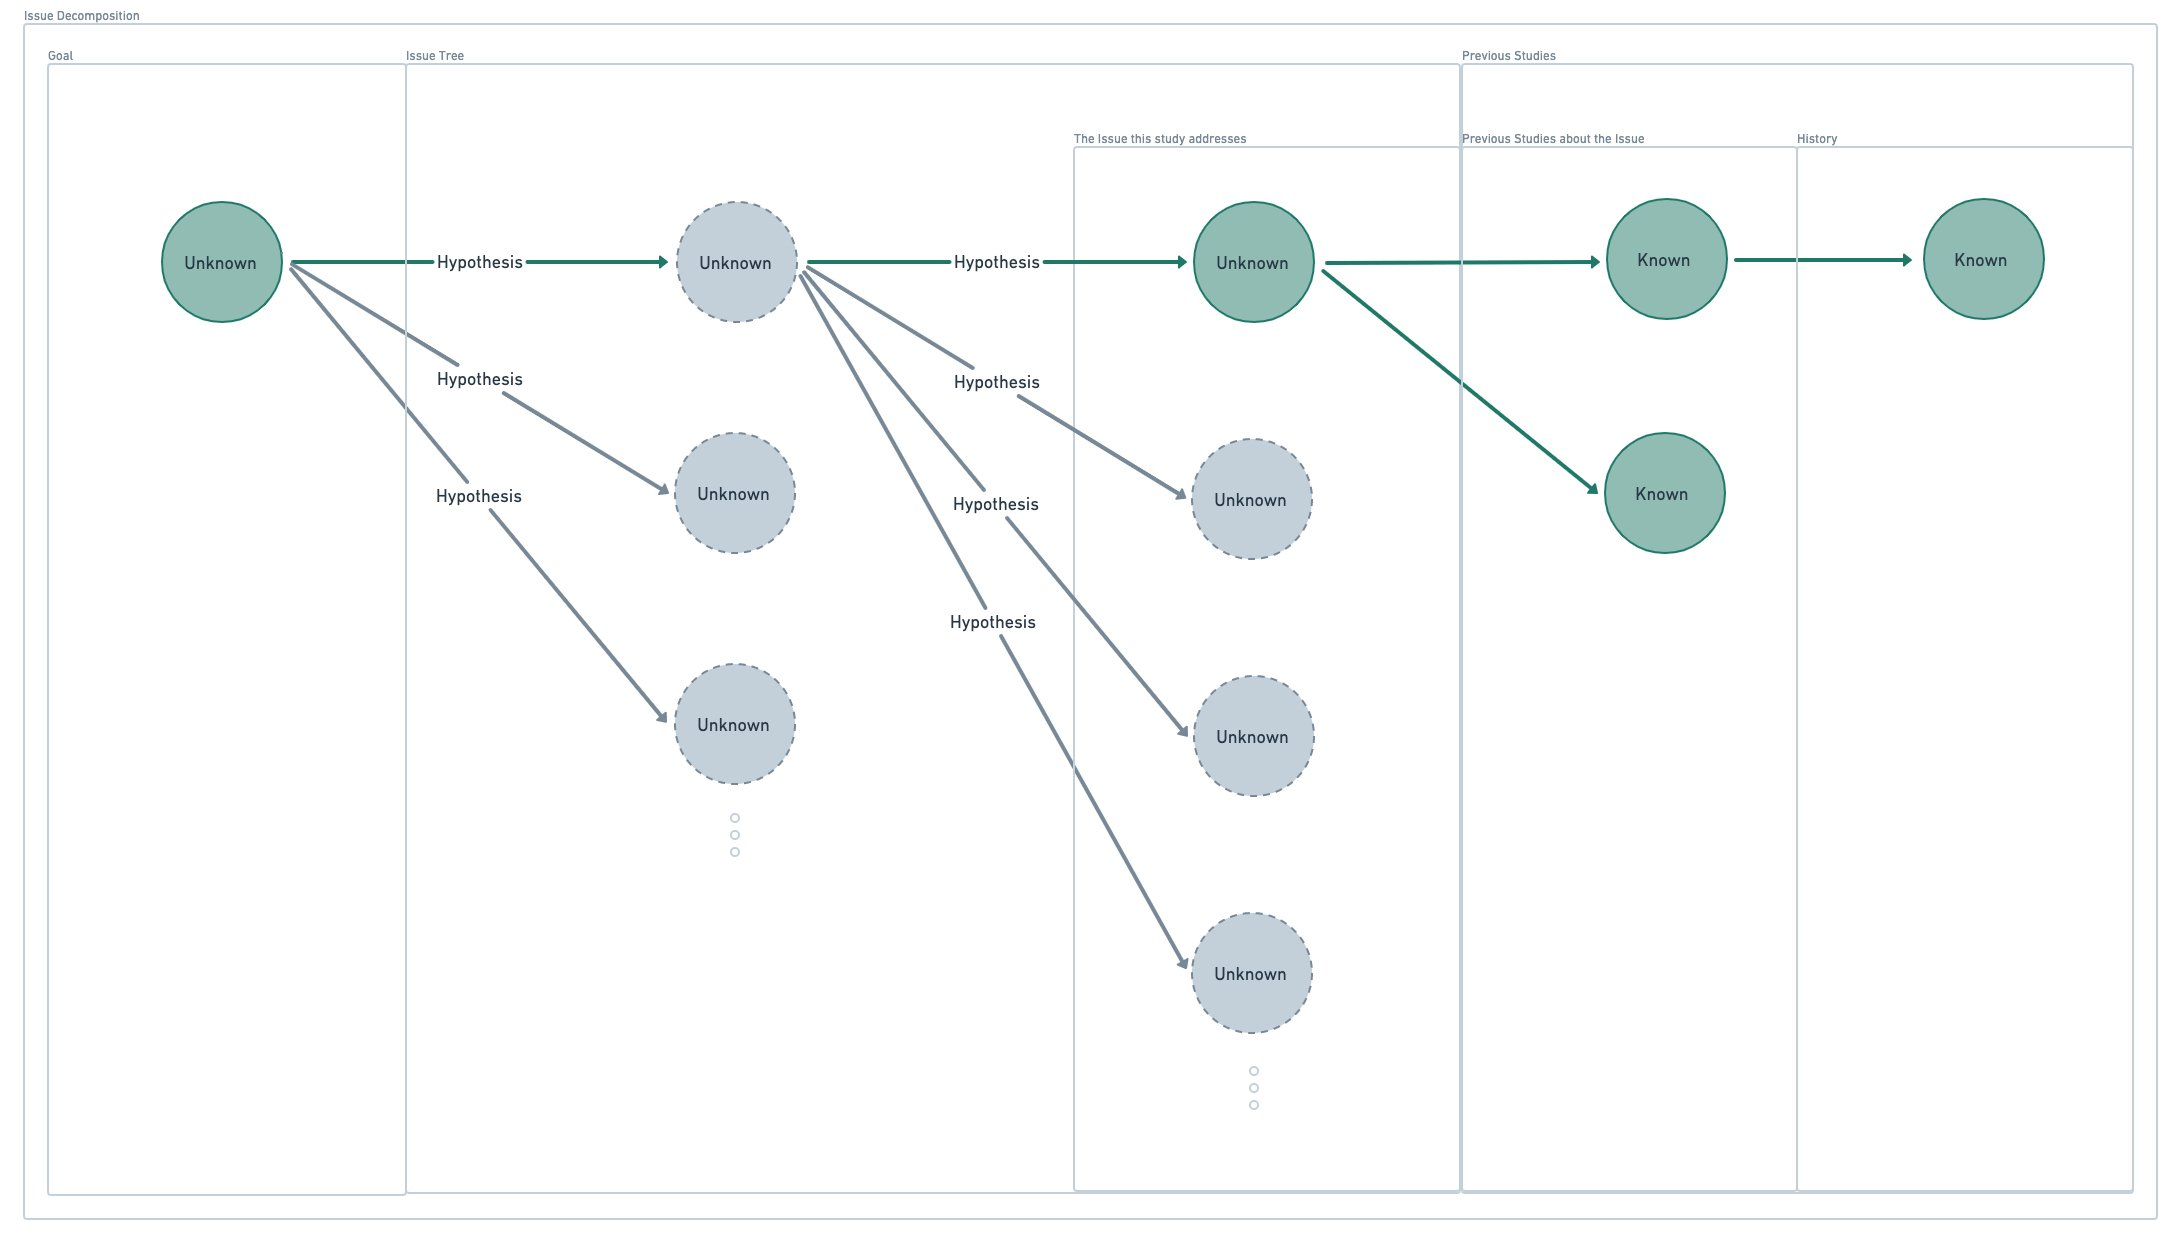
\includegraphics[width=\textwidth]{figs/unknown_tree.jpeg}
    \caption{Caption}
    \label{fig:unknown_tree}
\end{figure}

Several things are happening here. Firstly, listing the elements necessary for achieving the goal means generating sub-goals from the main goal. However, it's always a challenging problem to evaluate how a particular sub-goal contributes to the achievement of a given goal. Especially in the case of research, the target might be an too general and ambitious vision that nobody has achieved before, so we need to think about what needs to be done to break it down into appropriate sub-problems. In other words, it is necessary to construct a tree with nodes representing sub-goals. Namely, this is the tree of repetition of constructing a question and generating multiple hypotheses without verification. We will delve into the discussion of hypothesis generation in the next chapter, so we won't go into the details here.

Secondly, it is necessary to identify the most important and feasible sub-goal from the selected candidate sub-goals. This is because only one question can be addressed in the end. However, assessing and comparing sub-goals is a challenging task since we have no experience to realize the ultimate goal and so have no data what sub-goal actually is the most important.

Thirdly, the question to ultimately arrive at must be verifiable. If the question is not specific, meaningful verification cannot be performed. Overly broad or ambiguous questions can result in countless or trivial answers, or they may be too unclear to provide practical answers. Increasing the specificity of the question corresponds to deepening the depth of the sub-goal tree, so it may be important to construct a sufficiently deep tree and find an efficient way to navigate it. The verifiability is constrained by the knowledge, resources, such as funding and technology, that we currently have. Therefore, when conducting verification in reality, it is necessary to consider such feasibility. Whether to tackle a question with high feasibility or to further divide it into more sub-tasks for its realization is a matter of judgment. In any case, it is necessary to appropriately evaluate such feasibility. The scope of feasibility is vast, so it is a challenging problem to determine how to consider it in creating intelligent systems.

In this discussion, we considered the method of outputting questions from the goal through the construction and exploration of a tree structure. However, as mentioned by the predecessors, if an end-to-end approach ultimately becomes a powerful method, it may be more desirable to consider a direction in which questions are directly output from the goal. In particular, even when performing multi-step reasoning, it seems more natural to improve reasoning abilities using the recently developed approaches to multi-step logical reasoning, rather than explicitly considering tree structures. 

To pursue this direction in research automation, specifically, it may be worth considering the construction of higher-quality datasets for goals and research questions. For example, it may be possible to construct a dataset by extracting only the ultimate goal and the research questions actually solved from the introductions of papers. However, an important point to note here is that the research questions created by humans so far are not necessarily optimal for achieving research goals. Firstly, machines may be capable of maximizing the objective better than humans due to cognitive constraints. Secondly, not all human research has been conducted by working backward from a clear goal. Some studies were conducted simply because they seemed interesting while reading papers. In this regard, simply learning from human data may constrain the potential capabilities that machines can possess. Therefore, it becomes important to consider how to formulate the maximization of the probability of achieving research goals as a problem, rather than naive imitation learning of human data.

As evident from the formulation, to construct research questions for contributing to achieve a specific goal, we need to solve long range reasoning problems. This problem is widely studied in machine learning research community to improve the reasoning capabilities of machine learning models and on generate intermediate goals in reinforcement learning. If these research fields produce significant results, they can be directly applied. In this sense, it might be beneficial to seek cooperation from those who are actively conducting research in these areas. One of the unique aspects of long-distance reasoning problems in research automation is that the goal is something that has never been achieved before. This means that you cannot naively learn from data and need to generalize out of distribution. Therefore, it's essential to acquire skills not just to recognize patterns but to properly trace the path of reasoning. Moreover, because the goal has not been realized, sub-goals and the paths that connect them are ultimately based on the accumulation of hypothesis generation. In this sense, it can be said that this is a highly uncertain inference. This implies that the choice of which node to select is far from self-evident compared to other logical reasoning problems. Furthermore, there is the issue of the complexity of the distance between the goal and the question, which is far more intricate than, for example, games or planning everyday trips. For instance, to truly achieve the goal, it may be necessary to build large-scale apparatus like particle accelerators from scratch. This also means that the temporal distance between the goal and the current location is very long. Therefore, it becomes a problem that feedback on how much solving the question contributed to the goal is significantly delayed. While we've only listed a few examples here, there may be other unique challenges and issues that become more serious in research. It will be necessary to work on refining these technical challenges into specific research tasks through discussions with researchers in reasoning and planning.

\subsubsection{Important but Unnoticed Questions}

One example of a ``good'' question seems to be one that, in its construction itself, brings benefits to many people. The reasons why the answer to a question remains unknown are diverse. In some cases, the question is simply new, and no one has had the time to come up with an answer yet. For instance, a question about the internet posed on the day it was invented may still remain unanswered because it has only been a day since its birth, and no one may have delved into it yet. In other cases, the question might simply not interest anyone, leading to an absence of answers despite the availability of time. This is an example of a question that remains unanswered because nobody is willing to tackle it, even though time exists.

Furthermore, there are questions that are difficult, and no one has been able to solve them. For instance, the question of how to achieve human immortality has been contemplated by many, but due to its complexity, no answer has been found yet. Lastly, there are questions that are important for a particular purpose but remain unnoticed by everyone. As previously mentioned, realizing challenging objectives that are yet to be achieved poses difficult problems. In such cases, it is often unclear what is not known or what is at the heart of the problem. In such situations, clarifying the question itself holds great significance.

Thus, constructing questions of this kind seems to be important as it can help shed light on the unknown. With this in mind, it appears worthwhile to discuss this topic in detail. \footnote{
Please note that the concept of a question being unnoticed and the answer to the question being unknown are different. The necessary condition for research is that the answer to the question is unknown. 

If the existence of a question is not known to anyone, then naturally, its answer would also be unknown since no one would have answered it. So, if the existence of a question is unknown, then the answer to the question is also unknown.
}

\textcolor{red}{TODO: Add discussion}

% Multiple Reasons for Unknownness

% new, unimportant, difficult, unnoticed, ... etc.

% This means that we distinguish between questions that are ``good'' and those that are not, based on certain criteria. 

% This means that we distinguish between questions that are ``important'' and those that are not, based on certain criteria. For example, \cite{alon2009choose} claims that a good question is one that solves challenges facing the research community. Likewise, we consider a question to be important if it generates knowledge that greatly contributes to a certain purpose. Valuing the degree of contribution to a purpose also implies viewing research as a form of problem-solving. \textcolor{red}{TODO: Add explanation of what this sentence means}

% Thus, in realizing an agent that autonomously constructs questions, it may become important to consider how to automatically determine ``goodness'' of the questions. To achieve this, it would be important to first understand in more detail what kind of questions we consider ``good''. \textcolor{red}{TODO: Add possible directions}

% \subsubsection{How to Practically Construct a Question}

% There has been much discussion on how to actually generate questions. Off course, these discussions primarily focus on how to formulate good questions. Therefore, please note that the examples mentioned here are proposals for generating such kind of questions.

% One typical approach to formulating a research question is to conduct a literature survey, identify research gaps in existing studies, and propose a question that aims to fill those gaps.

% \textcolor{red}{TODO: Add survey of how to construct questions; gap spotting, problemization, etc}

% Next, let's consider the process of constructing purpose-driven research questions. When aiming to conduct impactful research, we believe that constructing purpose-driven research questions is crucial. In this approach, we first set the ultimate objective. Then, we identify the most critical bottlenecks, or sub-goals, that are essential to achieving that objective. We once again consider sub-goals for these identified bottlenecks. This process is repeated, converging on more specific and feasible sub-goals that are of high importance. Finally, we frame the question to address these sub-goals as the research question. 

% In practice, we seem to determine the questions we should tackle in this way, implicitly and explicitly. For example, let's say that someone try to answer a question of ``How neural networks have reasoning capability?'' in his/her study. This question may come from a thought process of ``we want to create artificial general intelligence, which requires systematic thinking, that needs ...'' In this case, the final purpose is to achieve ``artificial general intelligence'', and the question addressed as a result is ``ow neural networks have reasoning capability?'' In other words, when we want to conduct important research, we follow a process that starts with the goal we want to achieve, considers the tree of important unknowns that should be clarified for its achievement, and sets the end of that tree as the research question. This process is summarized in Fig. \ref{fig:unknown_tree}.


% Of course, the purpose mentioned here may be a sub-goal of a higher-level goal. For example, the goal of ``creating general artificial intelligence'' may be a sub-goal of a more fundamental goal of ``satisfying intellectual curiosity,'' and the goal of ``satisfying intellectual curiosity'' may be biologically demanded for better exploration of the environment. These can lead to an infinite regression when considered strictly, so we won't delve into it any further here, but it could become an important issue when considering how to realize fully autonomous agent to construct questions.

% \subsubsection{Question}

% The construction of a question is the act of seeking information \cite{watson2015ask}. Specifically, in the context of research, we consider information as knowledge. The act of seeking knowledge involves two steps: 1. Recognizing the lack of knowledge and 2. Attempting to fill that knowledge gap. In this discussion, we assume that intelligence is designed to consistently generate questions when given input. Therefore, we temporarily set aside the aspect of "triggering action" related to the second step of attempting to fill the knowledge gap.

% The recognition of a knowledge gap occurs when we expect to have certain knowledge and, upon referencing our accessible knowledge, we find that it is not available. For example, when running a program and encountering an error that we cannot resolve on our own, we recognize that we lack the necessary knowledge.

% The reasons for expecting the existence of certain knowledge can vary and are arbitrary. In this case, we assume that a purpose given by a third party creates an expectation of certain knowledge. For example, in the case of humans, we first consider what we need to do to achieve a certain purpose. We then anticipate the necessary knowledge to accomplish those tasks, and when we find that it is not present within our existing knowledge, we recognize the knowledge gap.

% Lastly, in this discussion, knowledge refers to the collective body of research findings, particularly academic papers. In actual research, a researcher may personally have a question and then investigate previous studies to confirm that it is indeed unknown before formulating it as a research question. However, what is important in the construction of a research question is that it is unknown to other entities. Therefore, for simplicity, we directly refer to the entirety of academic papers without including the step of comparing personal knowledge.

% To summarize, to create an intelligence capable of constructing questions in this setting, we need to design it to expect the necessary knowledge to achieve a given purpose provided by a third party, search for that knowledge in academic papers, assess whether the papers contain sufficient knowledge to achieve the purpose, and express any knowledge gaps as questions.

% In this case, we excluded the discussion of triggering action by design. However, when considering increasing autonomy, it is important to discuss how to incorporate this aspect into learning and acquisition. The question of "why do we seek information" has been extensively discussed in the context of curiosity.

% Furthermore, in this case, we defined the expectation of knowledge as aiming to achieve a given purpose. However, as mentioned earlier, this does not affect the formulation of questions. For example, let's consider the case of a child asking, ``Why is the sky blue?'' In this case, the child may already have prior knowledge of the concept of ``sky'' and ``blue.'' Additionally, they may possess a naive concept of causality, believing that ``A is B, so there must be a reason for it.'' Thus, they may have expected to have the knowledge that ``the sky is blue because of B.'' However, when they reference their internal knowledge, they find that it does not contain the corresponding knowledge. Therefore, they may have asked the question ``Why is the sky blue?'' to evoke the knowledge they were lacking.

% In this way, the reasons for expecting the existence of certain knowledge can vary, and what, why, and how we seek information (knowledge) are not constrained by specific conditions. Therefore, when attempting to create an intelligence capable of constructing questions in the future, it is feasible to develop a more flexible intelligence.

% Additionally, in this case, we assumed that the given purpose and its achievement are predefined goals. However, humans naturally set their own goals. When considering the design of a more autonomous intelligence, it is conceivable to aim for automation in this aspect as well. However, as mentioned earlier, the question of what we seek knowledge about is not specific to research. Therefore

% , we temporarily set it aside for now. If we were to pursue this direction further, it would ultimately lead to an infinite regress, raising the question of how much information to consider as given.


%%%%%%%%%%%%%%%%%% Rearangement %%%%%%%%%%%%%%%%%%%%%%%%%%%%

% \subsection{question construction}
% Research is an endeavor to bring the unknown closer to the known. Therefore, it is necessary to first determine what unknown we aim to make known. And this unknown often takes the form of questions. For example, ``Why do deep neural networks with a large number of parameters generalize well?'', ``How can we prevent the problem of vanishing gradients?'', and like these. These are commonly referred to as \textit{research questions} or \textit{research problems}. Therefore, in this paper, we will refer to the step of determining this unknown as \textit{question construction}.

% \textcolor{red}{TODO: should describe question construction itself first. What is research question or research problem?}

% \subsubsection{Unknownness}
% As we have reiterated, it is a necessary condition for research that the answer to a question is unknown, or in other words, that there is a high degree of uncertainty. Therefore, it is essential in research to have methods that ensure the answer to a posed question is truly unknown, or to formulate questions that truly have unknown answers.

% Knowledge for humanity is primarily disseminated through research outcomes. Therefore, when examining all the research outcomes that have been generated thus far and finding that none of them provide an answer to a specific question, it seems reasonable to conclude that the question possesses sufficient uncertainty to warrant further investigation as a research endeavor. In particular, humanity has developed the culture to preserve the research outcomes in the form of papers. Therefore, it seems feasible to assess the unknown nature of an inquiry by examining all academic papers. However, it is impossible to review them all due to constraints in terms of time, technology, and cognitive limitations. Therefore, it is realistic to consider a question as unknown if it has been sufficiently and comprehensively explored through an extensive examination of these academic papers. In practice, we conduct literature reviews to synthesize existing research, identify research gaps in existing studies, and thereby ascertain the unknowness of our own questions or construct question for which the answers are unknown \cite{schryen2015theory}. \textcolor{red}{TODO: Consider where we will explain about literature review}

% % In the previous statement, it was mentioned that as long as the unknown is truly unknown and it can be approached towards becoming known, there should be no problem. The process of approaching the known will be explained in the next section, and here we will delve a bit more into the determination of unknownness. 

% However, in reality, such rigorous literature research is not always conducted in every case. Currently, researchers often demonstrate the unknownness of the answer to the question by referencing only a few related works and explaining that none of them have yet resolved the unknown. And when the paper is evaluated by reviewers, who are a small group of experts, if it is determined that the question has indeed not been answered so far, the provisional recognition of the unknown nature of the question is granted. This means that a subjective evaluation criterion is being used, where researchers and a small number of reviewers consider a question as unknown when none of their known studies provide an answer.

% % This implies the use of subjective evaluation criteria, where researchers examine several papers considered ``major literature'' in a field and consider them as unknown if none of them have provided an answer. Furthermore, as mentioned later, we evaluate the quality of research outcomes by having them assessed by a small number of experts in the same field. If these researchers determine that the previous studies have been sufficiently comprehensive, the determination of unknownness is considered somewhat valid. In other words, ultimately, the evaluation by a few experts may serve as the basis for establishing the unknownness.

% This current convention stems from the cognitive constraint that there is a limit to the literature that humans can examine. Since unknownness is a fundamental aspect of research, ideally, it should be evaluated objectively and rigorously. For instance, it would be desirable to quantitatively state which journals, what types of papers, and how many have been examined, and the result indicating their unknownness. Although systematic reviews already employ such approaches, there is, of course, a limit to the number of papers that can be evaluated manually and selection biases cannot be removed. \textcolor{red}{TODO: Add the explanation of systematic review, problems of it, and how AI can mitigate them.}

\subsubsection{Diverse Good Questions}
There have been various discussions on the elements that good research possesses. For example, \cite{hulley2007designing} proposed that good research question should satisfies FINER criteria (feasible, interesting, novel, ethical, and relevant) and \cite{alon2009choose} claims that a good problem is one that is most feasible and interesting to oneself.

\textcolor{red}{TODO: Add more discussion on ``good'' questions, examples, discussion, what is good, what is important, specific question is good, etc.}

% However, we have not found a unified consensus on the definition of good question. but 

% \subsubsection{Questioning as Information Seeking Behavior}
% \textcolor{red}{TODO: Reconstruct}

% The construction of a question is the act of seeking information \cite{watson2015ask}. Specifically, in the context of research, we consider information as knowledge. The act of seeking knowledge involves two steps: 1. Recognizing the lack of knowledge and 2. Attempting to fill that knowledge gap. In this discussion, we assume that intelligence is designed to consistently generate questions when given input. Therefore, we temporarily set aside the aspect of "triggering action" related to the second step of attempting to fill the knowledge gap.

% The recognition of a knowledge gap occurs when we expect to have certain knowledge and, upon referencing our accessible knowledge, we find that it is not available. For example, when running a program and encountering an error that we cannot resolve on our own, we recognize that we lack the necessary knowledge.

% The reasons for expecting the existence of certain knowledge can vary and are arbitrary. In this case, we assume that a purpose given by a third party creates an expectation of certain knowledge. For example, in the case of humans, we first consider what we need to do to achieve a certain purpose. We then anticipate the necessary knowledge to accomplish those tasks, and when we find that it is not present within our existing knowledge, we recognize the knowledge gap.

% Lastly, in this discussion, knowledge refers to the collective body of research findings, particularly academic papers. In actual research, a researcher may personally have a question and then investigate previous studies to confirm that it is indeed unknown before formulating it as a research question. However, what is important in the construction of a research question is that it is unknown to other entities. Therefore, for simplicity, we directly refer to the entirety of academic papers without including the step of comparing personal knowledge.

% To summarize, to create an intelligence capable of constructing questions in this setting, we need to design it to expect the necessary knowledge to achieve a given purpose provided by a third party, search for that knowledge in academic papers, assess whether the papers contain sufficient knowledge to achieve the purpose, and express any knowledge gaps as questions.

% \begin{figure}[htb]
%     \centering
%     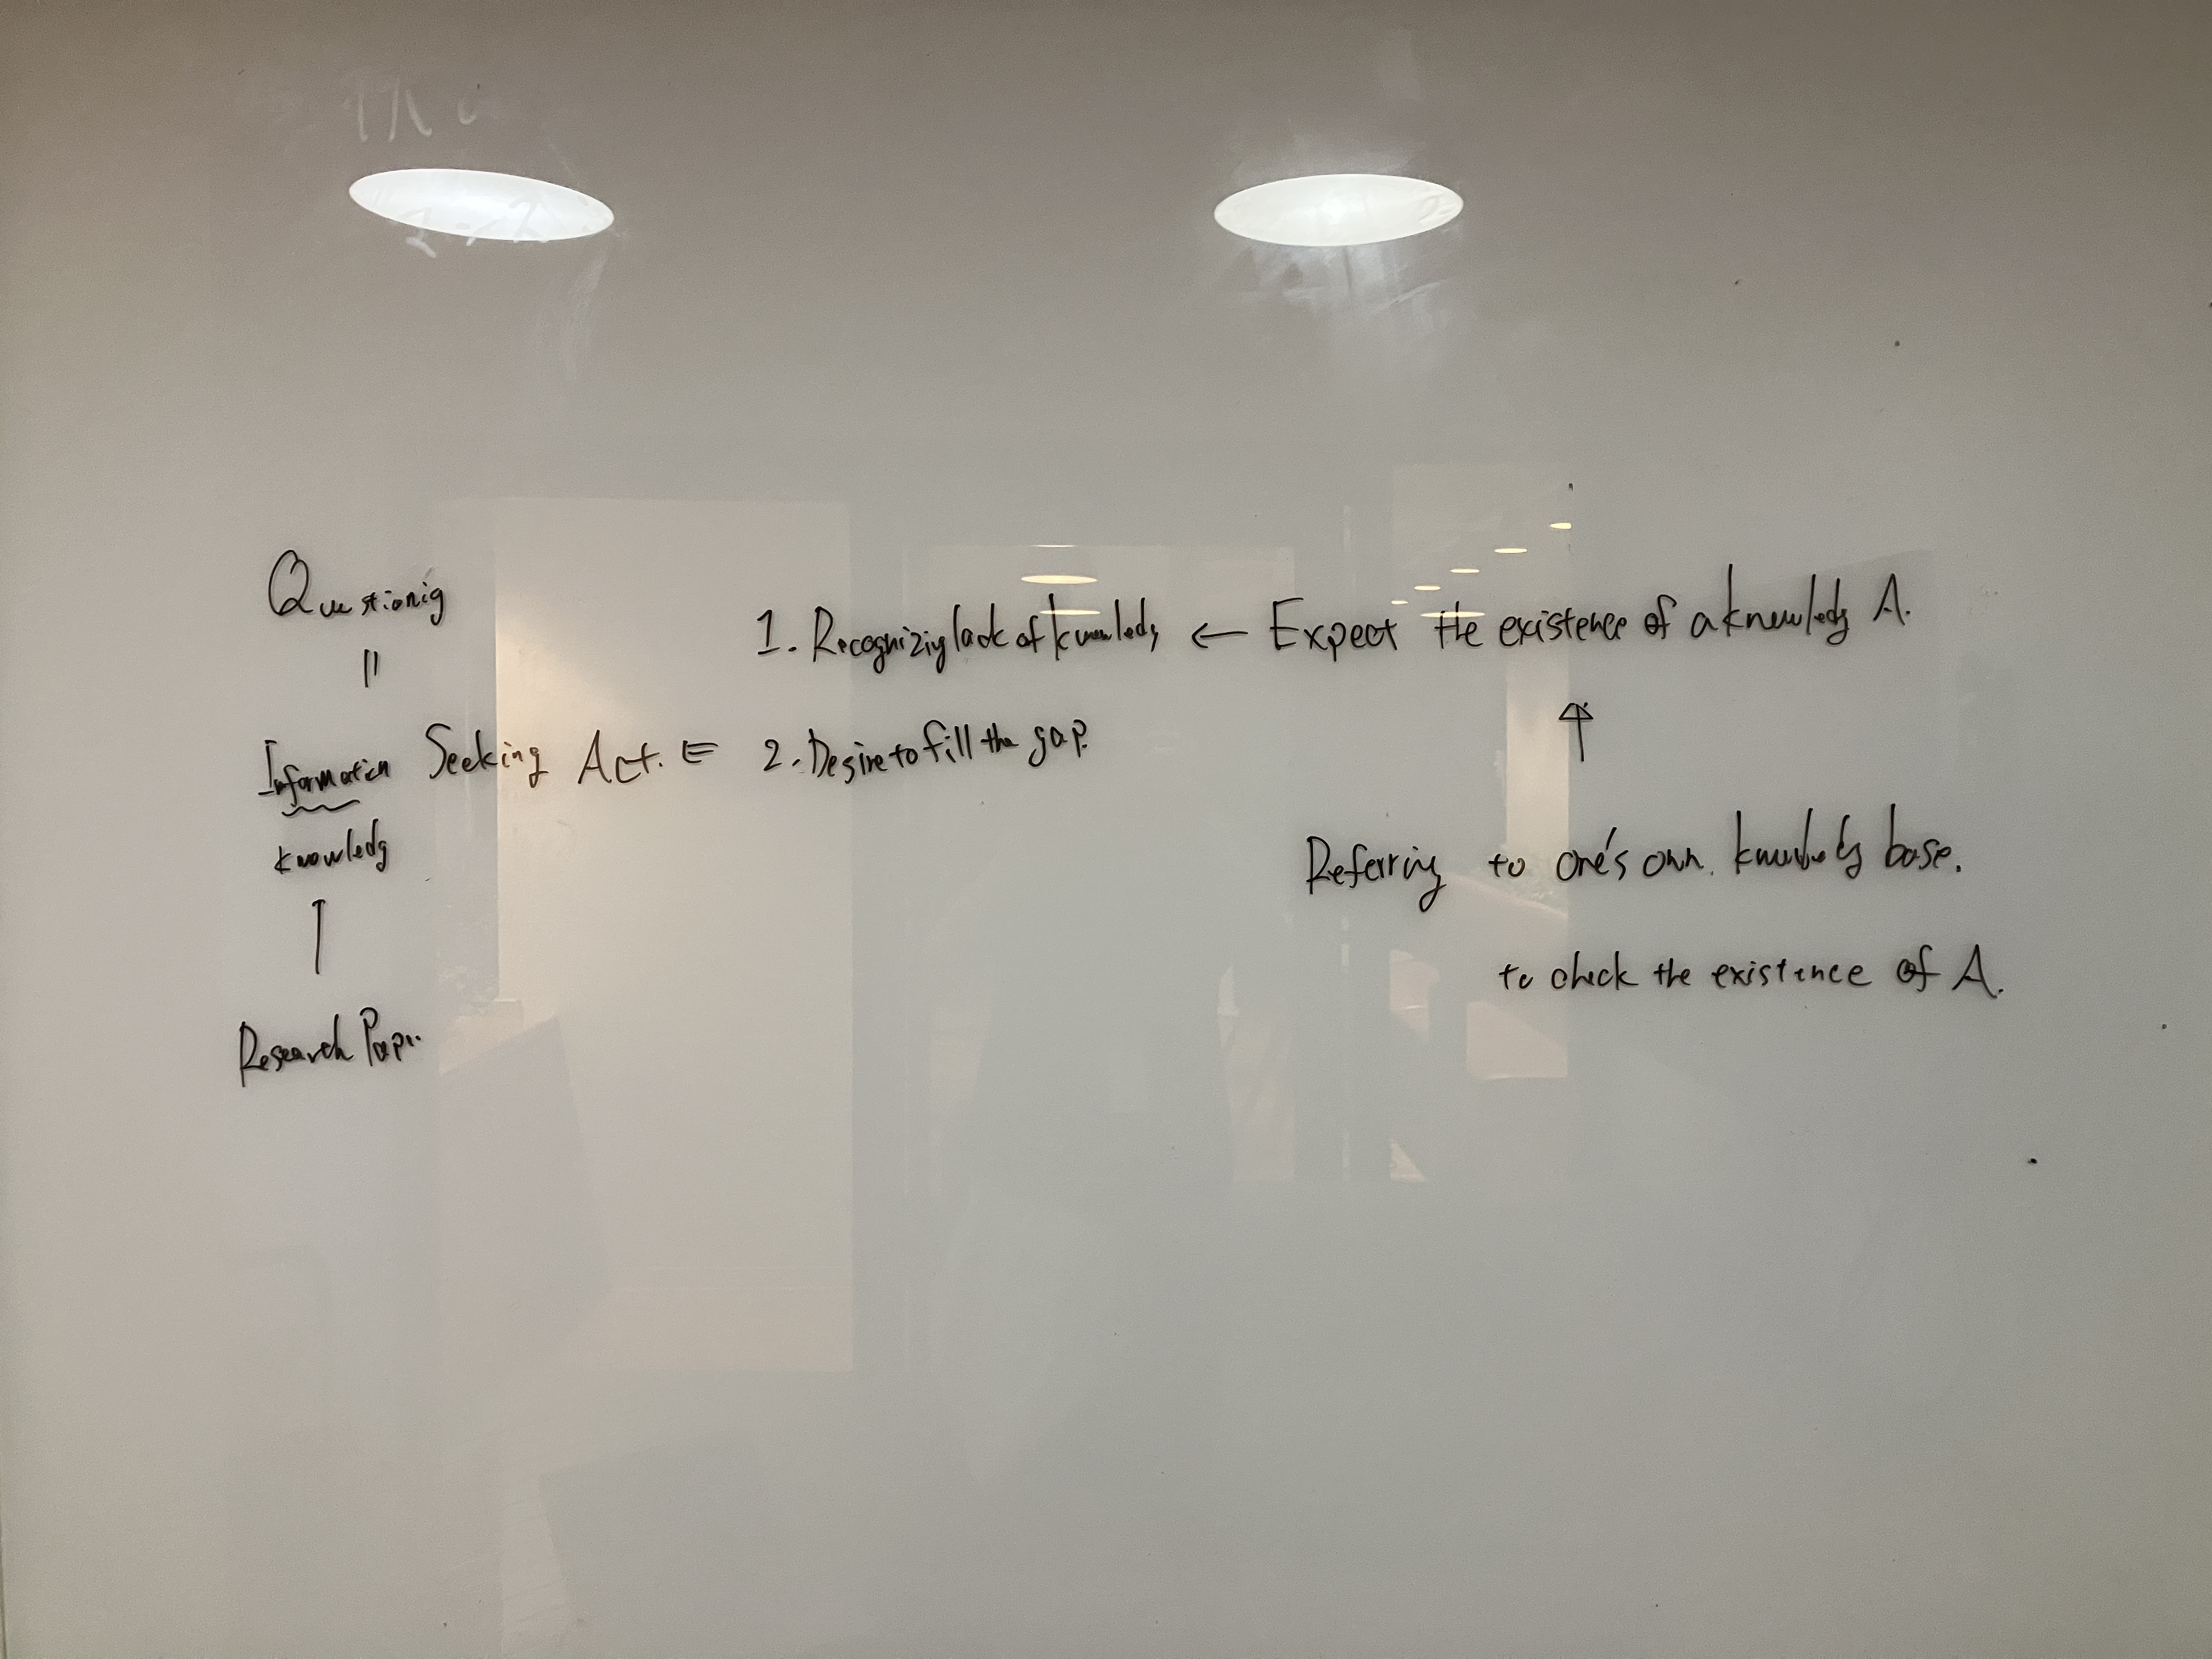
\includegraphics[width=\textwidth]{figs/question_formulation.jpg}
%     \caption{question construction}
%     \label{fig:enter-label}
% \end{figure}

% \textcolor{red}{TODO: Is question construction information retrieval??}


% Asking questions is an act of seeking information \cite{watson2015ask}. The act of seeking information (or knowledge) arises from realizing the lack of one's own knowledge and the desire to fill that gap. Therefore, to create intelligence that can autonomously ask questions, it is necessary to incorporate mechanisms that induce these behaviors.

% Determining what triggers this behavior in humans is a challenging problem. However, when designing a system, it is sufficient if it can induce such behavior, regardless of what it actually is. The principle that ``behavior is triggered when it is somehow desirable for the agent'' represents this idea. You are probably familiar with this concept in reinforcement learning, where rewards (desirability of actions) are provided, and maximizing the expected value of these rewards is formulated as an appropriate way to induce behavior.

% The notion of triggering behavior by realizing the lack of one's own knowledge and attempting to fill it has been extensively studied in the context of curiosity in the field of reinforcement learning. In research, agents that pose questions can generally be formulated within this framework.

% \subsection{question construction}
% The construction of a question is the act of seeking information \cite{watson2015ask}. Specifically, in the context of research, we consider information as knowledge. The act of seeking knowledge involves two steps: 1. Recognizing the lack of knowledge and 2. Attempting to fill that knowledge gap. In this discussion, we assume that intelligence is designed to consistently generate questions when given input. Therefore, we temporarily set aside the aspect of "triggering action" related to the second step of attempting to fill the knowledge gap.

% The recognition of a knowledge gap occurs when we expect to have certain knowledge and, upon referencing our accessible knowledge, we find that it is not available. For example, when running a program and encountering an error that we cannot resolve on our own, we recognize that we lack the necessary knowledge.

% The reasons for expecting the existence of certain knowledge can vary and are arbitrary. In this case, we assume that a purpose given by a third party creates an expectation of certain knowledge. For example, in the case of humans, we first consider what we need to do to achieve a certain purpose. We then anticipate the necessary knowledge to accomplish those tasks, and when we find that it is not present within our existing knowledge, we recognize the knowledge gap.

% Lastly, in this discussion, knowledge refers to the collective body of research findings, particularly academic papers. In actual research, a researcher may personally have a question and then investigate previous studies to confirm that it is indeed unknown before formulating it as a research question. However, what is important in the construction of a research question is that it is unknown to other entities. Therefore, for simplicity, we directly refer to the entirety of academic papers without including the step of comparing personal knowledge.

% To summarize, to create an intelligence capable of constructing questions in this setting, we need to design it to expect the necessary knowledge to achieve a given purpose provided by a third party, search for that knowledge in academic papers, assess whether the papers contain sufficient knowledge to achieve the purpose, and express any knowledge gaps as questions.

% In this case, we excluded the discussion of triggering action by design. However, when considering increasing autonomy, it is important to discuss how to incorporate this aspect into learning and acquisition. The question of "why do we seek information" has been extensively discussed in the context of curiosity.

% Furthermore, in this case, we defined the expectation of knowledge as aiming to achieve a given purpose. However, as mentioned earlier, this does not affect the formulation of questions. For example, let's consider the case of a child asking, ``Why is the sky blue?'' In this case, the child may already have prior knowledge of the concept of ``sky'' and ``blue.'' Additionally, they may possess a naive concept of causality, believing that ``A is B, so there must be a reason for it.'' Thus, they may have expected to have the knowledge that ``the sky is blue because of B.'' However, when they reference their internal knowledge, they find that it does not contain the corresponding knowledge. Therefore, they may have asked the question ``Why is the sky blue?'' to evoke the knowledge they were lacking.

% In this way, the reasons for expecting the existence of certain knowledge can vary, and what, why, and how we seek information (knowledge) are not constrained by specific conditions. Therefore, when attempting to create an intelligence capable of constructing questions in the future, it is feasible to develop a more flexible intelligence.

% Additionally, in this case, we assumed that the given purpose and its achievement are predefined goals. However, humans naturally set their own goals. When considering the design of a more autonomous intelligence, it is conceivable to aim for automation in this aspect as well. However, as mentioned earlier, the question of what we seek knowledge about is not specific to research. Therefore

% , we temporarily set it aside for now. If we were to pursue this direction further, it would ultimately lead to an infinite regress, raising the question of how much information to consider as given.

% \begin{figure}[htb]
%     \centering
%     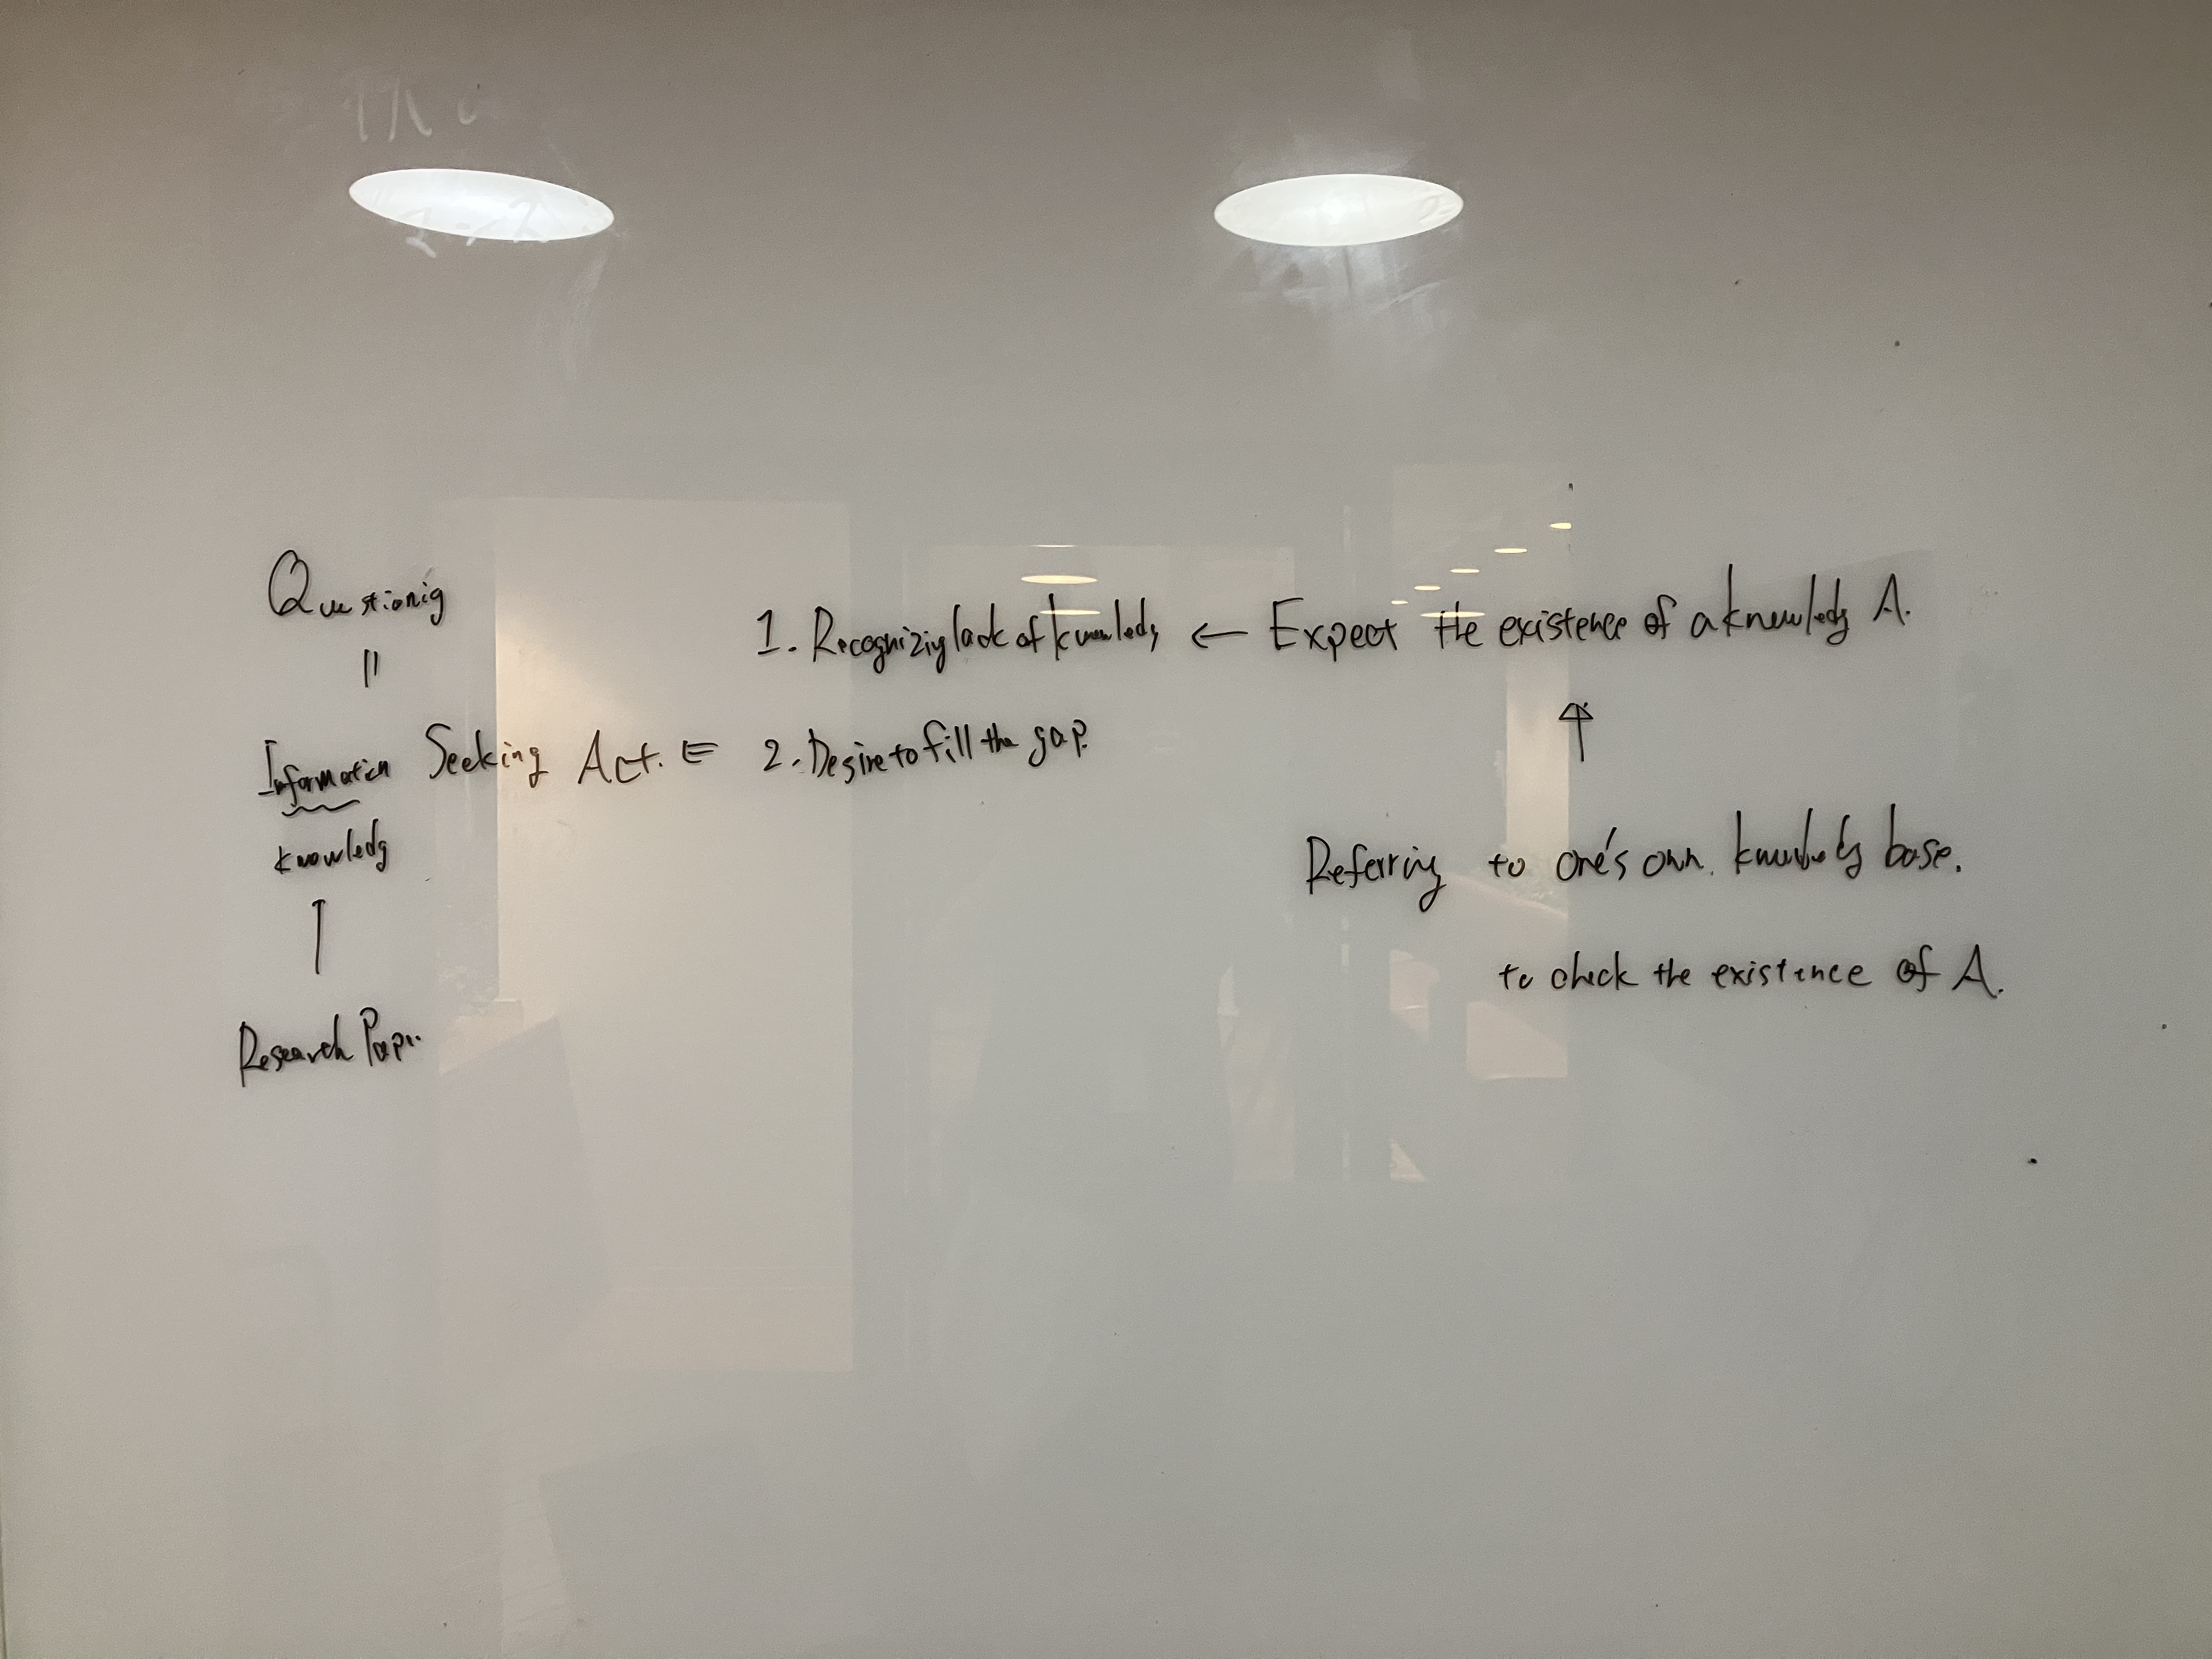
\includegraphics[width=\textwidth]{figs/question_formulation.jpg}
%     \caption{question construction}
%     \label{fig:enter-label}
% \end{figure}


% \textcolor{red}{TODO: Is question construction information retrieval??}


% \subsection{Conclusion}

% \begin{enumerate}
%     \item Determing the existence of expected knowledge:
%     \begin{enumerate}
%         \item Searching for knowledge directly related to the expected knowledge.
%         \item Determining whether the knowledge has been properly validated.
%     \end{enumerate}
% \end{enumerate}

% 1.b is specific to the automation of research. 





% We have listed what we believe are important elements in the construction of questions. However, these are considered important under the assumptions mentioned earlier. For instance, if the goal is not to acquire knowledge necessary for achieving an objective, but to generate knowledge that an individual finds interesting, the necessary elements in question construction (particularly in parts 1.a and 1.b) would change. As previously mentioned, the value of knowledge is determined in relation to context and there's a high degree of uncertainty about how the value of knowledge will evolve in the future. This makes it fundamentally important to have a diverse range of ways to generate questions. The object achievement is highly prevalent and is expected to produce ``important'' knowledge, which is why it is discussed here. However, it is important to discuss what other ways of formulating questions could exist and how they can be implemented.

\section{Hypothesis Generation}
We began by explaining that we first formulate the unknown we are addressing in the form of a question. The process of finding answers to this question is research. Here, because the answer to this question is, of course, unknown, it requires inference as to what the answer could be. As a result of this inference, a plausible answer is formulated. This process corresponds to the \textit{hypothesis generation}. Hypothesis generation is the inference about the unknown and the definition of research is to transform unknown to known. Thus, every research including deductive research must entail hypothesis generation implicitly or explicitly. In this sense, hypothesis generation should be the second module of knowledge production system.

The belief that a hypothesis is true is the very object that can become knowledge in response to a question. If a hypothesis withstands proper testing, the belief in its plausibility strengthens. Conversely, if a hypothesis does not withstand testing, that belief is weakened. Therefore, the former generates knowledge that ``the answer to question A is hypothesis B,'' while the latter generates knowledge that ``the answer to question A is not hypothesis B.'' 

Hypothesis generation is the act of creating potential answers to a question, so naturally, it is essential to generate plausible hypotheses that are close to the actual answer. Therefore, let's start by referring to how humans generate hypotheses and then discuss how we can generate reliable hypotheses, drawing inspiration from human methods.

\subsection{Generating Plausible Hypothesis}
% \subsection{Hypothesis Generation: Proposal}
% As mentioned earlier, from the perspective of knowledge production, we believe that hypotheses are sufficient in principle if they fulfill the function of providing provisional answers to questions. However, in order to avoid unnecessary testing, it is important to derive ``plausible'' hypotheses. There are various approaches to this, but to provide some food for thought, we would like to share our personal view on how humans generate hypotheses.

Hypothesis generation is sometimes considered an unanalyzable, emergent process or a result of genius. However, we believe that human-generated hypotheses are produced through a process of trial and error in rational inference. In the following discussion, for the sake of simplicity, we will focus on hypothesis generation for why questions. \footnote{
Please note that not all research questions are why questions (e.g., ``Does life exist beyond Earth?'' is not a why question, but it is a scientifically investigable question).
}

% \subsection{Plausible Hypothesis and Unknownness}

% While predictions that are highly unlikely to be confirmed, such as random guesses, can still qualify as research, they do not contribute much knowledge because they are expected to be easily rejected without undergoing rigorous testing. It becomes a waste of resources to invest in validating such predictions. Therefore, it seems to be crucial for ``meaningful'' research to propose hypotheses that are somewhat plausible.

% It is immediately evident that this is a non-trivial problem. This is because research, despite being an endeavor to answer unanswered questions, requires considering plausible candidate answers for those questions. Here, if the unknown under investigation is entirely unrelated to existing knowledge, it is impossible to make meaningful predictions about it. This is because predictions are based on experiences and data. In other words, high novelty and high uncertainty indicate a complex structure that cannot be immediately predicted from past knowledge and experiences. It implies that constructing plausible hypotheses necessitates the ability to discern these complex structures and patterns from past experiences. While it is difficult to determine what is unknown and what constitutes a complex structure, these can be crucial points to consider when advancing the automation of research.

\subsubsection{Analyzing Question}
Researchers start with a question, the composition of which has been discussed in the previous section. Given the question, we break down the content of the question and analyze each part in detail. For example, let's say we have a question, ``Why are apples red?'' The first thing we would consider is what an apple is and what red means. We would also think about what it means for something to be red. Then, we focus on the properties of apples and the color red and abstract them. We may also think about other red things besides apples. If we already know the reason why tomatoes are red before knowing why apples are red, we might consider that the reason for tomatoes being red could apply to apples as well. By conducting this kind of analysis, we can connect our understanding to existing similar knowledge and attempt to explain using those existing reasons. These ways of focusing on abstract structural similarities between specific concepts and inferring that what can be said about A, which has the same structure, can also be said about B is called \textit{analogical reasoning}. This has been considered to be important method in hypothesis generation \cite{hesse1965models,thagard_1984,gentner1993shift,holyoak1996mental,dunbar1997scientists}.

For those simple examples given above, one can easily find analogical examples. However, many of the questions researchers actually grapple with are much more complex, and it's not immediately clear how they relate to existing knowledge. Even in such situations, researchers have managed to generate plausible hypotheses by analyzing research question thoroughly.

Such thorough analysis of questions seems particularly important when it comes to making significant discoveries that are remembered in history. Let's consider Charles Darwin as an example, who proposed the concept of natural selection. Darwin appears to have gone through a process of trial and error before arriving at the idea of natural selection \cite{gribbin2022origin}. After returning from his voyage on the HMS Beagle, he began to question how evolution occurs. It seems that he read the works of Lyell and Linnaeus, and particularly from Lyell's writings, he realized the importance of selection in evolution. The question then shifted to what could serve as a natural equivalent of artificial selection. Later, after reading Malthus' book on population, Darwin understood that in nature, competition leads to the preservation of advantageous species and the extinction of disadvantageous ones, which is the process of natural selection.

In essence, Darwin initially had the question of ``how does evolution occur,'' but through analyzing this question, referring to previous research, and conducting experimentations and observations, the question transformed into ``what is the equivalent of artificial selection in nature?.'' And it was through this transformation of the question that he was able to recognize the similarities between Malthus' discussion on human society and the mechanism he was seeking. Although the process is complex, this is the same as the hypothesis generation process we explained above in that he analyzed and transformed the question, finding analogies with existing knowledge and reaching a plausible hypothesis.

In the case of Darwin, it involved a more observational approach within the field of natural history, which prompted the transformation of his question. However, in fields such as theoretical research that utilize mathematics, different methods may be employed. For example, consider the scenario where there are two theories, theory A and theory B, and the goal is to achieve a unified description between them. In this case, one might repeatedly perform mathematical transformations on the objects described by each theory, reducing the significant problem of ``incompatibility between Theory A and Theory B'' to inconsistencies between specific properties of each theory. By introducing axioms that resolve these inconsistencies, it may be possible to construct a unified theory. It is important to reiterate that in cases where the subject matter is mathematically described, formal operations can be applied to objects of interest, such as object A and object B, to transform them into different forms. This process can lead to the discovery of unexpected similarities. It is through this approach that one can discuss the similarities between objects even when they may defy intuition or cannot be imagined through empirical means. 

Therefore, we believe that thorough analysis of question plays a powerful role in identifying similarities between objects, especially in cases where it is necessary to discuss the similarities between objects that may not be intuitively evident or imagined through experience. We believe that this is the core of the human hypothesis generation.

\subsubsection{Confirming Plausibility in Hypothesis Generation}

In the previous chapter, we explained how we transform questions by analyzing them and connecting them with existing knowledge. However, there seem to be countless ways to bring about changes in the questions. So, how exactly do we go about transforming the questions? Let's now describe the process of question transformation that we have in mind.

% In simple cases like ``apples are red,'' it may be sufficient to apply existing knowledge. However, in research, especially when tackling challenging questions, we believe that the following steps are involved. 

First, from the knowledge at hand, we select several hypotheses that are strongly related to the question and have a high level of confidence, and then proceed with accepting these hypotheses as premises. For example, the existing knowledge that tomatoes are red for reason A, strawberries are red for reason B  are strongly linked with the proposition that apples are red for reason C by the presence of the word ``red.'' Let's assume that we have a high level of confidence in the proposition that tomatoes are red for reason A, but only a low level of confidence in the proposition that strawberries are red for reason B. In this case, the reason A for tomatoes being red would be selected as the premise. \footnote{
In the case of humans, it may not always be the case that we prioritize knowledge with a high level of confidence. For example, let's consider a situation where we have recently read a book and acquired some highly impactful knowledge. In this scenario, even during the process of question analysis, we might be inclined to consider using this newly acquired knowledge because it has left a strong impression on us. This inclination is not solely based on its level of confidence, but rather because the knowledge has made a lasting impression, leading us to take it as a premise while analyzing the question. Like this, determining what knowledge humans choose to adopt as premises is a complex issue, and we refrain from delving into this issue in this paper.
}

Next, we will not focus on the parts of the question that pertain to the meaning of the premises or the deduced results that answer them. For example, going back to Darwin's example, when Darwin read Lyell's book, he took the proposition that ``selection matters in evolution'' as a premise. As a result, he left aside the question of ``what is important for evolution.'' Instead, he shifted his focus to solving the question of ``how does nature make selections?''

Once a certain premise is accepted, the next step involves examining the consistency between the consequences brought about by that assumption and one's existing knowledge. If introducing that premise does not lead to contradictions with strongly held beliefs, then the introduction of the premise is deemed acceptable. On the other hand, if introducing the premise results in contradictions with one's existing knowledge, it becomes a matter of choosing between the two. 

% This involves comparing the consequences brought about by the introduction of that premise with retaining one's existing knowledge and selecting the one that seems more favorable in some sense. For instance, Kepler compared the consequences of introducing the assumption of circular motion for planets with observational data and the results of his proofs, and eventually decided to discard the assumption of circular motion.

% or generating hypotheses that maintain consistency with this knowledge. Specifically, we generate hypotheses that seem relevant, and then verify that they do not contradict existing knowledge.

By considering the relationships between existing knowledge and new knowledge, and reevaluating which ones are deemed more plausible, one can undergo a process of transforming the question into its more essential form and generating plausible hypotheses. We seem to generate plausible hypothesis by transforming the question in like these steps.

\subsubsection{Continuity between Hypothesis Generation and Hypothesis Verification}

From the explanation so far, it becomes evident that in order to generate ``plausible'' hypotheses, we are conducting operations that involve changing our beliefs about the truth of those hypotheses. This seems natural since generating ``plausible'' hypotheses inherently involves such belief updates. However, this observation may offer significant insights into our current discussion. We define knowledge production as the updating of beliefs, which includes the construction of questions, the generation of hypotheses, and the operation we refer to as hypothesis testing, where we update our belief about whether a hypothesis is true. The implication of this discussion is that the process of generating ``plausible'' hypotheses and hypothesis testing share similarities. In reality, there are cases where hypothesis generation and justification are tightly connected in research practice \cite{arabatzis2006inextricability}. This leads to the question of whether we need to separate the processes of hypothesis generation and hypothesis testing.

However, we do not think that the fact that a single process play roles for both hypothesis generation and verification means that they are also play the same role for knowledge production. We believe that hypothesis generation and verification play two distinct role for knowledge production, and that's why we discuss separate them as two distinct modules.

You may say that it is not entirely implausible to interpret both hypothesis generation and verification as being ``belief updates.'' Certainly, this similarity becomes more evident, particularly when contemplating the generation of ``probable'' hypotheses. For instance, let's consider a scenario where belief values are continuous. In this case, generating a hypothesis involves changing the belief value of a certain hypothesis from its original value of, say, 0 to something like 0.1. Subsequently, if multiple hypothesis candidates are considered, and one is chosen as probable based on previous research, the belief in this hypothesis might increase to around 0.3. Through the final verification of this hypothesis, the belief might reach approximately 0.9, resulting in the formation of knowledge. From this perspective, hypothesis generation and verification can be seen as the process of modifying beliefs.

However, when aiming for knowledge production within a specific society, there is a distinction. During the verification phase, the beliefs that are updated are shared beliefs. In contrast, during the generation of probable hypotheses, the updating of shared beliefs is not required. Consequently, in the context of knowledge production, hypothesis generation generates beliefs that can be updated, while hypothesis verification serves as the means to update those beliefs, thus playing distinct roles.

% \subsection{Continuity between Hypothesis Generation and Verification}
% So far, we have emphasized that hypothesis generation and hypothesis testing are functionally distinct, and that seems somewhat reasonable. However, when considering the generation of "plausible" hypotheses, these boundaries become somewhat ambiguous.

% Since testing incurs costs, in reality, humans carefully choose hypotheses worthy of testing. Even after hypothesis testing is made more efficient by machines, narrowing down hypotheses to a certain extent remains practically essential. Therefore, this is a problem that persists even after knowledge generation is achieved through machines.

% When considering the generation of ``plausible'' hypotheses, it simply means strengthening the certainty about the truth or falsehood of a hypothesis. In other words, in terms of changing the belief about the truth or falsehood of a hypothesis, this can be seen as similar to testing. For example, in experimental research, we believe there is often a pilot study conducted before starting full-scale experiments. This is nothing more than evaluating whether the hypothesis is worth pursuing for rigorous testing.

% Therefore, it may be possible to identify hypothesis generation and hypothesis testing as being synonymous in the sense of belief updating. However, we still believe that there are differences between hypothesis generation and hypothesis testing. The confidence in hypothesis generation is ultimately a matter of individual researchers or those involved in the research, and it is not necessary for all members of society to share that confidence. On the other hand, testing requires methods that update the common beliefs of members of society. Therefore, while hypothesis generation and hypothesis testing can be regarded as equivalent in terms of belief updating, they may differ in the strength of that belief.

% Obviously it is not possible to consider the consistency for all possible knowledge, so in practice, researchers seem to be checking the consistency of the hypotheses with several studies or knowledge that they have in mind. The knowledge  may be the recent interesting papers they have read, knowledge they strongly believe in, and so on. The knowledge that comes to the researcher's mind at that moment and is prioritized in their thinking is likely to become the premises for these hypotheses. 

% In highly mathematicalized disciplines like physics, for example, one might judge the plausibility of a hypothesis by comparing the deduced consequences from that hypothesis with existing knowledge. In this way, hypotheses that are judged to be somewhat consistent with the assumed premises may be recognized as ``plausible'' and worthy of rigorous testing. Of course, there are factors other than the plausibility of a hypothesis that can affect its ``value,'' but we believe that plausibility is the most important value in terms of knowledge production.

\subsection{Hypothesis Generation from Verification Results}
So far, we have been discussing the process of generating hypotheses by analyzing a given question. In this case, the hypotheses are intended to answer the question from start to finish. However, in reality, we may end up generating hypotheses that are for completely different questions than the one we initially set out to solve. Surprisingly, some of these serendipitously generated hypotheses can become profoundly important and leave a mark in history. Let's take a moment to consider how such hypotheses are generated through this process.

Such hypotheses are born while attempting to identify the causes of verification results. Once a hypothesis is generated, the validity of it is assessed through hypothesis testing. In actual research practice, even if hypothesis testing yields negative results, it does not necessarily mean that the proposed hypothesis is completely discarded. Instead, supplementary premises may be introduced into the initially proposed hypothesis, and the modified hypothesis may be retested. On the other hand, it is also possible that the assumptions of the hypothesis are reconsidered, leading to the generation of new hypotheses. These are all practices of researchers involved in hypothesis generation, so let us explain them in more detail.

First, when humans think about something, they always need some assumptions. These assumptions refer to the knowledge or beliefs that individuals provisionally consider as ``correct.'' For example, when interpreting data at hand, one may assume that the measuring instrument used to generate the data is reliable, or that the principles of classical mechanics used for data collection are valid, or that the insights from several previous studies are valid. Additionally, researchers often introduce auxiliary hypotheses implicitly or explicitly during their investigations. For example, tentatively decided hyperparameters or auxiliary hypotheses introduced during calculations also become premises. Furthermore, there are implicit or explicit guiding principles and beliefs, such as the belief that ``hypotheses should be simple'' or that ``theories should be beautiful,'' which serve as premises for hypothesis derivation as well.

When verification yields negative results, all these assumptions, including the ones that are implicit, can be the cause for the result. The proposed main hypothesis itself may be incorrect, the auxiliary hypotheses may be incorrect, or the observations may be incorrect. Researchers must identify which of these possibilities is the cause. This is known as the problem of Duhem-Quine's thesis \cite{sep-scientific-underdetermination}. This is like trying to generate hypothesis on the question of ``What is the cause of the error?''. As you can understand, this is an extremely challenging problem since this is like debugging a system that is unstructured, where the entire code is not visible, and there is no systematic approach, and you have to grope in the dark. 

In practice, it seems that humans adopt a strategy of revising beliefs from the weakest ones first to tackle this proble. This strategy, in our opinion, is somewhat reasonable and rational. For example, let's say the parameters introduced in this study were chosen arbitrarily. This could be one of the first things to be revised because there is no reason for it to be that way. However, just because something was introduced in this study does not mean it will always be revised. For example, if results from the hypothesis under investigation are remarkably consistent with the background assumptions, we should keep the hypothesis. Alternatively, let's say the verification results are not completely off track but slightly deviated. In such cases, the fact that the verification results were negative may not make it reasonable to completely discard the hypothesis. The researcher may add terms or ad-hoc assumptions only to resolve those small errors or inconsistencies.

On the other hand, if, for example, the hypothesis of this study is based on classical mechanics, it would not be reconsidered unless there is a substantial reason to do so. Classical mechanics has been shown to be highly consistent with an immense amount of knowledge based on it, so revisiting it unconditionally would require an explanation sufficient to negate the entire system. In this sense, researchers will have a fairly strong belief in the validity of classical mechanics. The important point here is that, regardless of the reasons, when a researcher has a strong belief or takes certain assumptions for granted to the extent that they no longer doubt them, the priority of revisiting those assumptions is diminished. For example, during the time of Johannes Kepler, the belief that planetary orbits were perfect circles was widely shared as an unquestionable assumption. Therefore, it took considerable trial and error before Kepler started to question that assumption. Believing that planetary orbits are perfect circles and believing in the validity of classical mechanics are vastly different in terms of the reasons for belief, but they share the common aspect that researchers at the time strongly believe the principle, revisiting those assumptions would not occur unless there is a substantial reason to doubt them.

In this way, researchers start by revising less firmly held beliefs first and repeat this process until contradictions are resolved. In our opinion, this is a somewhat reasonable strategy. Of course, as with the belief in the circular orbits of planets in Kepler's time, there are beliefs that are implicitly assumed but not verified, and researchers still hold these beliefs. However, many strong beliefs are directed toward knowledge that has withstood numerous tests, and in that sense, it seems natural to first attribute the cause to weaker beliefs than to these strong beliefs.

Thinking in this way, we can understand why mathematics has played a crucial role in science. First and foremost, in mathematics, it is necessary to state the assumptions explicitly. Therefore, among all the potential influencing assumptions, only the assumptions under consideration are represented as mathematical objects. Furthermore, mathematics is a deductive system, so if any contradictions arise in the results, we can conclude that one of the assumed premises must be incorrect as long as the inference rules are correctly applied. Consequently, we can confine the process, which could have an infinite number of causes, to a finite and debuggable system for discussion. Additionally, when verifying the consistency of a hypothesis with the underlying assumptions used to generate it, the relationship of how the hypothesis is deduced from those assumptions can also be mathematically examined. This allows us to proceed with confidence, understanding the reasons why and to what extent we need to question each assumption. Finally, mathematics is abstract so is help us to find the analogical relationships. We believe these factors have hugely contributed for humans to generate plausible question.



% In research, a hypothesis is a prediction of the answer to a question that no one knows the answer to. Therefore, a ``good'' hypothesis is primarily one that represents the true answer to the question. To generate such a ``good'' hypothesis, we need to consider several factors. Here, we would like to discuss the reasons for the unknown that we previously discussed. Easy questions naturally lead to the generation of good hypotheses, and there is not much meaning in discussing the quality of hypotheses in such situations. Therefore, in this context, we will focus on how to generate ``good'' hypotheses for difficult questions that many people are challenging but have not yet been answered.

% we do not precisely know what it means for a question to be difficult. However, if we consider an analogy with machine learning, inference about patterns that rarely occur in the training data is challenging. Therefore, difficult questions may correspond to the tail part of the distribution during the training phase in machine learning or cases where there is a distribution shift (specifically, when the true distribution is mistakenly inferred during training). If that is the case, the ability to appropriately infer hidden patterns without being misled by spurious correlations in past experiences could be crucial in generating ``good'' hypotheses for difficult questions.

% Humans have employed various means to solve this difficulty. One approach is to incorporate new perspectives by borrowing knowledge from other fields or old papers. As we accumulate knowledge for research, we implicitly acquire the dominant ways of looking at things in that era. While it may not be false correlation, it undoubtedly makes certain patterns less visible. Bringing in insights from unrelated fields to the current domain might relativize these perspectives and provide a trigger to notice hidden patterns. Another approach is to leverage the power of mathematics. For example, in the field of physics, hypotheses for a certain question are built as theories with the help of mathematical tools. This involves deductive operations at various points, allowing for leaps of inference that go beyond human past experiences. We have also utilized various techniques such as analogies and the use of computers. However, all of these methods have been human approaches to overcoming broad out-of-distribution generalization.

\textcolor{red}{TODO}


\subsection{Hypothesis Generation by Machines}

Within a single process of knowledge production, they serve the role of being subject to verification and are mere beliefs if not tested or refuted. However, when considering the entire ecosystem of knowledge production, hypotheses play an extremely important role. This is because research is the act of generating new knowledge based on past knowledge and hypotheses are potential knowledge, justifying them indirectly influences future knowledge production.

\subsubsection{What is Necessary for Hypothesis Generating Machine}
As we have been stating repeatedly, hypothesis generation is a prediction based on experience. More specifically, one could formulate hypothesis generation currently performed by humans as a broader question-answering task. If that is the case, what requirements are there for creating a machine learning model that generates research hypotheses, beyond just a question-answering task? Particularly, is it merely a result of human cognitive constraints that we explicitly transform a question statement to find analogies, or is this an important aspect in hypothesis generation not limited to humans?

The answer to this seems to vary depending on who the question's answer is unknown to. Firstly, let's discuss the scenario where the answer to the question is unknown to humanity. This scenario corresponds to utilizing artificial intelligence just for a hypothesis generator for humans. In this case, it may not necessarily be required for machines to undergo the intermediate step of explicitly converting the question, as it is possible for them to directly generate an answer to the question. This is because what is unknown to humans may already be known or obvious to machines. Currently, artificial intelligence demonstrates capabilities that surpass human abilities, and as their capabilities continue to advance, this trend is likely to accelerate further. It is important to note that even in cases where a direct answer is provided without explicit question transformation, as you may already be aware, there is an implicit process of transformation occurring.

Next, let's discuss the scenario where the answer to the question is unknown to the machine itself. This corresponds to the situation where artificial intelligence engages in research to explore the unknown from its own perspective. Here, artificial intelligence aims to generate knowledge rather than being a tool for human research. In this case, we hypothesize that explicitly performing question transformation is important in hypothesis generation for machines, even if it doesn't need to be done in the same way as humans. If the most plausible answer for a question is always correct for the machine, it can be said that the question was not unknown to the machine in the first place. Therefore, paradoxically, if a question is unknown to the machine, it means that the machine needs to employ some means to extract patterns or structures that it is not capturing from the question. This is similar to situations where a machine is overfitting, being misled by spurious correlations, or failing to extract the patterns it should extract due to lack of out-of-distribution generalization. These are issues that will inevitably arise as long as machine learning continues to focus on minimizing errors as its central objective. For a machine to autonomously engage in research, it needs to be aware of being in such a situation and take actions to grasp the currently unapprehended patterns. Analyzing the question and converting it into a different form to facilitate the discovery of unknown patterns is precisely one of the most fundamental efforts in this regard. Therefore, it appears crucial for a machine to undergo such transformations in order to autonomously engage in research.

On the other hand, in many large-scale language models currently in existence, it seems to be a fundamental principle that what others consider plausible knowledge is deemed plausible as well. For example, widely used techniques like instruction tuning involve supervised learning where the training data consists of human or machine responses. In essence, the optimal solution is to mimic the behavior of these agents. Similarly, RLHF (Reinforcement Learning from Human Feedback) essentially learns to consider as correct what the labelers have deemed correct. In both cases, the common aspect is that the reward or training data tends to mimic the behavior of other agents in society.

The problem that arises here is whether such learning processes can lead to the proposal of innovative hypotheses. For example, during the time of Kepler, most people believed that planets move in circular orbits. If a machine trained in such an era, reflecting the biases of those people, were to generate hypotheses, it would likely exhibit a bias towards supporting circular orbits. Therefore, it seems that more than just accepting what many people say as correct, some criteria, goals, or frameworks beyond that are necessary.

As mentioned earlier, mathematics has been a powerful tool for freeing humans from such biases. Regardless of one's strong personal beliefs, the strength of deduction lies in the necessity of accepting the results that emerge from appropriate formal operations. Thus, it seems crucial in hypothesis generation to possess the ability to manipulate some form of deductive or formal system, even if it is not the same mathematical system as humans.

Another aspect that can be learned from human examples is that humans determine their level of confidence in knowledge through their own validation or tracking the validation conducted by others. This is closely related to the topic of verification, which will be discussed in the next section. Humans read books, papers, and other sources, carefully examining the claims and the verification processes presented in them. When they judge these sources to be trustworthy, there seem to be a significant number of individuals who increase their confidence in the validity of that knowledge, regardless of how it may differ from common sense. This attitude contrasts with the attitude of ``it's correct because many people say so'' and is referred to as a scientific and critical attitude. And, as I mentioned earlier, I believe this attitude can be rephrased as an approach that evaluates the reliability of knowledge through verification. Without such an attitude, it would be difficult to propose innovative hypotheses that challenge established theories. Therefore, the ability to verify hypotheses, as explained in the next section, also seems important in creating machines that generate ``plausible'' hypotheses.

\subsubsection{Conclusion}
In this section, we have presented a hypothesis that the tasks involved in hypothesis generation may vary depending on who the answer to the question is unknown to. If the answer to a hypothesis is unknown to humans, it may be sufficient for the machine to generate questions directly based on the hypothesis. However, if the answer to a hypothesis is unknown to the machine, we have suggested that the machine needs to analyze and appropriately transform the hypothesis.

Nevertheless, it is worth noting that the aspects discussed above can also be useful in the context of hypothesis generation for humans.

\subsection{Hypothesis, Understanding, and Explanation}

% If it were not necessary to make inferences about the unknown, it would probably be because the question was not unknown in the first place. Thus that is not research by definition. It may not be explicitly stated, but as long as it is research, it implicitly involves some form of hypothesis generation. Therefore, the generation of a hypothesis, or the inference about the unknown, is essential for research in nature. Let's say, mathematics, a pure deductive field of research. In searching for lemmas to prove a theorem, we sometimes make predictions such as ``this lemma might be useful'' and examine it with few specific examples to check its usefulness. This may be considered as implicitly establishing a hypothesis and roughly verifying it. 

% In particular, science, by explicitly dividing the proposal of this plausible temporary answer and the corroboration of its tentative certainty into steps known as hypothesis generation and hypothesis verification, has enabled these processes to be carried out more systematically and rigorously. This is the well-known hypothesis-testing method, or scientific method. In this approach, a prediction about the unknown is explicitly stated as a hypothesis, and a procedure called verification is established to evaluate the validity of this hypothesis. Through this verification process, the evaluation of the hypothesis is conducted and the uncertainty towards the target unknown is reduced. This is the knowledge production based on the hypothesis testing method. 

% As a practice of human science, there are cases where discovery and justification are not strictly separate in actual scientific endeavors \cite{arabatzis2006inextricability}. However, functionally, discovery and justification can be classified separately, and it seems convenient to consider them as distinct in knowledge production that is not dependent on human conventions. Therefore, we will discuss them separately here.

% Although we said that hypothesis generation is the important part of scientific method, the hypothesis generation is not necessarily unique to the empirical science. It is a task that inevitably arises when dealing with the unknown. 

% \subsubsection{Note on Unknown}
% Let us make a note here about the term unknown again. We wrote that if an answer can be immediately derived by inference, it was not unknown in the first place. However, research is an activity to transform the unknown into the known, so in some form, unknown should eventually approach the known (reducing uncertainty). Moreover, if there is something that seems to be completely unrelated to the known or experiences (though it is hard to imagine), it seems inherently impossible to bring it closer to the known. In that sense, it is reasonable to think that the unknown has some relationship with the known. Therefore, the above description might be more accurate if it refers to cases where the confidence in the answer is lower, or the path to the answer is complex, and uncertainty is high. This is similar to the discussion on the definition of unknown in the previous section.

\subsection{\textcolor{red}{Existing Discussion on Hypothesis Generation}}
\textcolor{red}{TODO: add studies}

%%%%%%

Since 19th centuries, the act of producing knowledge, in particular hypothesis, and that of verification of it have been distinguished as the context of discovery and context of justification \cite{sep-scientific-discovery}. And during the most of the 20th centuries, the discovery caught much less attention by philosophers of science. 

In engineering discussions, there is often explicit formulation of sets or candidates of hypotheses, and the discovery of hypotheses in such situations is often discussed \cite{simon1973does,kitano2021nobel,bengio2022ml4sci}. However, when automating hypothesis generation it is also important to consider how such candidates arise in the first place. There have been attempts to understand this process, such as highlighting the importance of analogy \cite{thagard1984conceptual} or mental model \cite{nersessian1999model}, but the question of how to generate ``good'' hypotheses still remains unanswered. The generation of initial hypothesis candidates has been discussed in the context of creativity in science. As you are well aware, however, current machine learning models are already capable of executing creative tasks effectively \cite{sep-creativity}. Thus, there is a debate about how much emphasis should be placed on creativity when considering the development of artificial intelligence capable of generating new hypotheses.

% \subsubsection{Good Hypothesis}

\subsection{Machine Prediction and Hypothesis}
We have explained that hypothesis generation is inference about the unknown, in other words, it is a prediction. Thus, in terms of its functionality to knowledge production, it is sufficient if a agent can do prediction. As you all know, machine learning models are functions to do predictions about unknown data. In this sense, prediction by machine learning can be equated with the generation of hypotheses. Therefore, when considering the automation of research, hypothesis generation can be dealt with as just a prediction task in a broad sense. As emphasized above, what we aim for is not merely imitating human knowledge production, but rather the autonomous practice of knowledge production that is not bound by human conventions. From that perspective, the act of generating hypotheses may be assimilated into a larger category rather than simply being labeled as prediction.

The issue that becomes important here is the problem of representing knowledge and hypotheses. As mentioned earlier, research is the process of generating knowledge for a society constructed by certain agents. Therefore, it is necessary for the produced knowledge to be interpretable, or at least usable, by at least some members of the society, even if not by all of them. In human society, it seems that knowledge is made possible by expressing it in a form understandable to the members of the society, such as natural language or mathematical language.

we stated that hypotheses are simply predictions. However, even if their validity is verified in a manner that other members find acceptable, if the content of those predictions cannot be interpreted, it seems that the predictions generated there cannot be called "knowledge of that society." This is because common beliefs are not formed. It may not necessarily be the method currently adopted by human society, but it seems necessary to adopt a form of representation that all members can interpret the content in some way.

% As emphasized above, what we aim for is not merely imitating human knowledge production, but rather the autonomous practice of knowledge production that is not bound by human conventions. And in terms of its functionality, hypothesis generation is identical to inference towards the unknown. In that sense, while understanding how humans generate hypotheses can be very useful in considering how to achieve effective hypothesis generation, we do not consider it is always necessary.

% Of course, hypothesis may have additional constraints on top of the prediction. For instance, there might be an implicit assumption that a hypothesis is something described in natural language. However, we think this is only due to the conventions of current human society. What is functionally important for the purpose of knowledge production is to provide a tentative answer to the unknown, regardless of its form or property. In this sense, in this paper, we take the position that hypothesis generation is the prediction.

\textcolor{red}{This (commented out sentences) is about hypothesis generation automation so will be moved to survey section of perspective section}
% Indeed, much of the current discourse on hypothesis generation focuses on specific research domains or discusses the exploration of hypotheses based on hypotheses that humans have explicitly defined. We understand this situation because hypothesis is an answer to a tentative question and hence it varies depending on the question. For example, if a study aims to enhance our understanding of a particular phenomenon, then the description or mechanism of that phenomenon would become the hypothesis. Similarly, if the objective is to solve a particular problem, then the solution to that problem would be considered the hypothesis. However, it is essential to consider how we can realize agents that construct candidates rather than just search for them, regardless of the specific research domain. This is a crucial question to address when contemplating artificial researchers.

\subsection{Prediction, Explanation, and Understanding}
Humans, in order to derive hypotheses in response to questions, often require thinking and deliberation on why those hypotheses are considered plausible. Without such cognitive processes, it is difficult to generate hypotheses in many cases. This is not merely a cognitive constraint; it has played a significant role in the advancement of research. The explanation of how a hypothesis is derived and the reasoning behind its plausibility have provided crucial additional information for understanding the subject of study. This has assisted people in gaining a better understanding of the phenomenon.

As mentioned earlier, predictions do not necessarily require such processes. Even without explanations for how such predictions arise, one can make inferences, and if they are rigorously tested, they can be considered knowledge. However, knowledge lacking such important additional information is expected to contribute less to the understanding of other knowledge and the comprehension of the entities targeted by the knowledge system. This research and understanding problem becomes significant even when artificial intelligence engages in research.

\textcolor{red}{TODO: Add more}

% \subsubsection{Others}

% In engineering research, as part of new knowledge, it is often required to propose actual design plans or algorithms. This can be considered as having a similar function to a hypothesis in the sense that it is a proposal for addressing a problem and is evaluated in some way.

% In mathematical research, proving a theorem that was previously unknown is the production of knowledge. However, since mathematics is a deductive system, if the proof is correctly executed, it can be said to be ``correct'' in that sense. In other words, the proof itself is both the proposal and the verification. Therefore, mathematics is not a type of work that separates hypothesis and verification.

\section{Hypothesis Verification}

\textcolor{red}{TODO: add detailed explanation}

we consider verification to be a particularly crucial process in the generation of knowledge. Questions and hypotheses can be generated in arbitrary ways, and they can take any form. However, verification must not be taken like this. Verification must be done in a manner that can convincingly update the shared beliefs of other members of society. Therefore, it is the most demanding process in the research journey in terms of rigor and caution. We believe that the rigor of this process is what truly sets research apart from other activities. The rigor and systematicity of the verification process is considered the very reason why science or research is referred to as rigorous in many cases \cite{sep-scientific-method,hoyningen2008systematicity,haack2003defending}.

we also recognize that the verification process is the most flexible and variable stage, as it can significantly differ depending on the subject of research. For instance, if one wishes to study the behavior of rat, they may need to train the rat, whereas investigating elementary particles may require the use of elementary particle accelerators. In the field of history, the existence of historical records might serve as evidence, while in mathematics, the verification process revolves around the proofs themselves. Due to this high degree of flexibility, we think that this stage becomes the most challenging aspect in automating research processes.

\subsection{How to Justify Beliefs}
In many empirical sciences, statistical methods occupy a privileged position as the primary means of verifying hypotheses. Therefore, it seems important to consider in what sense we can say that a statistical method can validate hypotheses, while we admit that the methods of verification vary greatly depending on the type of question or hypothesis and it cannot be said that there is any universal method for verification. The use of inferential statistics methods is widely accepted, but it is a challenging issue to known how various statistical techniques, each with their own approach, can provide evidence to substantiate a hypothesis based on the data in the real world \cite{otsuka2022thinking,sober2008evidence,sep-statistics}. Thus, what constitutes the verification of a hypothesis, or in other words, the justification of a belief, is a very difficult debate in which it is likely challenging to arrive at a unified answer. Please note that the discussions mentioned earlier, such as the uniformity of nature, pertain to the validity of induction itself. In statistical methods, however, induction is assumed and the discussion begins with formulating this uniformity by assuming a probability model. 


This discussion of statistical method provides important insights for the pursuit of developing AI capable of conducting autonomous research. As can be seen from the assumption of being rooted in machine learning, the validity of inductive inference itself is generally accepted and not a practical concern in creating such AI. However, how to make agents acquire the methods of justification is a important issue. If the criterion for justifying beliefs is to be acquired completely autonomously from scratch, it may very well lead to criteria that are meaningless for humans. Additionally, it seems that the criteria for justification employed by humans are diverse. When properly considering the reasons that these criteria are believed to provide justification, we can recognize that there are highly intricate structures involved. In light of such considerations, the extent to which one can understand and acquire criteria for justification from the criteria humans already employ is a nontrivial problem. Even empirical sciences, which employ highly universal verification methods based on statistical approaches, face such difficulties. Therefore, aiming for autonomous acquisition of verification methods in broader fields of research would likely pose even greater challenges. These issues will require further in-depth discussions in the future.

\subsection{Uncertainty of Verification}
Verification is a highly challenging process when examined closely. Firstly, as mentioned earlier, inductive approaches cannot verify hypotheses in the same way as deductive reasoning. Also, we notice that hypothetico-deductive method, which involves verifying claims derived from a hypothesis to confirm its validity, is still widely used today. However, verifying a deduced claim does not support the hypothesis because there may be many hypothesis that can result in the same deduced claim. In response to these, Karl Popper proposed that while hypotheses cannot be confirmed, they can be falsified \cite{sep-scientific-method}. However, in practice, the verification of hypotheses involves implicitly relying on numerous auxiliary hypotheses. When using experimental apparatus, it requires many assumptions to trust them. Even when an experiment fails, determining whether the hypothesis was incorrect or the experiment itself was flawed is not as straightforward as one might think. Thus, there is inherent uncertainty in attributing the results of verification to a specific cause \cite{chalmers2013thing,sep-physics-experiment,sep-scientific-underdetermination}. Furthermore, all reasoning and observational evidence are inevitably influenced by some form of theories, individuals, or societal factors \cite{sep-science-theory-observation}. Therefore, it is necessary to carefully examine them to ensure that they are not distorted by unintended influences. \textcolor{red}{TODO: add more}

we do not intend to claim that these uncertainties undermine the reliability of research. Such uncertainties exist in almost all human endeavors. Research, among these activities, strives to confront these uncertainties with great care and rigor. Above all, the fact that the results generated through research have effectively supported our lives demonstrates their efficacy.

we mentioned the difficulties inherent in verification to highlight their significance, particularly when considering autonomous artificial intelligence capable of self-verification. Ideally, autonomous agents are expected to establish their own methods and criteria for verification. However, if verification inherently carries such difficulties and uncertainties, the more rigorously we consider it, the more paralyzed the agent becomes, as it seemingly cannot accomplish anything. \textcolor{red}{TODO: Add explanation}

% A characteristics of research can be found in the systematicity, rigor, and objectivity of research practice \cite{sep-scientific-method,hoyningen2008systematicity,haack2003defending}. 

% In particular, we believe that a characteristic of research lies not in the way of determining questions or generating hypotheses, but in the fact that the verification of hypotheses is done in an extremely rigorous and careful manner. 

% It could be said that I'm taking a view similar to the new experimentalism, placing emphasis on verification in research, or experiments \cite{chalmers2013thing,mayo1996error}.

% Of course, generating a hypothesis is not a simple task. What we want to say is that, as long as any method of hypothesis generation is properly verified, it is considered research, and no matter how properly a hypothesis is proposed, if the verification is sloppy, it is not considered research. This means that verification may be at the heart of knowledge production. In other words, in order to create artificial intelligence that produces knowledge, it is important to consider how to create an intelligence that can perform verification.

\subsection{Towards Autonomous Verification}
\textcolor{red}{TODO: May be moved to perspective chapter?}

As mentioned above, we believe that the process of verification is highly diverse. Therefore, achieving an end-to-end approach immediately is difficult, and we think it requires even stronger constraints, at least in the short term, compared to other processes. For a practical first step for the verification process automation, we propose tentatively dividing the verification process into three stages: \textit{verification design}, \textit{verification instantiation}, and \textit{verification execution}. Then, the verification execution can be broadly categorized into the processes of data generation and data analysis, while this categorization may apply for only empirical sciences. \textcolor{red}{TODO: Add Fig}

\textbf{Verification Design.} At this stage, we contemplate how to validate the hypotheses and proceed to formulate a verification plan. In a verification plan, the agent writes about the hypotheses, verification criteria (what will be considered as evidence for verification), and the procedures for conducting the verification. Going beyond a high-level description, it may be beneficial to write these plans in as much detail and procedural clarity as possible. The Fig. provides an example in the context of machine learning. The idea is to create a blueprint for a pipeline where verification is automatically executed by faithfully following the plan. We consider this important because the verification process offers a high degree of flexibility, making it extremely challenging to achieve an end-to-end automation, at least in the short term. \textcolor{red}{TODO: Add Fig}

Furthermore, for artificial intelligence to perform autonomous verification, it seems essential that the AI not only adopts certain verification criteria but also be able to explain the meaning behind them and how they contribute to the verification process. Even humans may sometimes engage in this without conscious awareness, such as conducting hypothesis testing because ``everyone does it.'' In that sense, this requirement may be somewhat challenging. However, if the aim is to truly enable AI to autonomously conduct research, it appears crucial for the AI to have a proper understanding of what constitutes verification and be able to design it itself or, at the very least, explain it adequately.

\textbf{Verification Instantiation.} At this stage, the research plan that has been developed is translated into an executable instance. For example, if the research plan states, ``Train the model B with the dataset A...'' the necessary steps would involve acquiring dataset A from the appropriate source, formatting it to be compatible with the model's input requirements, and preparing the data for training, etc. Similarly, if the plan states, ``When a rat presses the switch B, food is dispensed...'' the agent has to prepare rats, food, and create a machine that dispenses food upon pressing the switch, and so on. This process involves translating the plan, expressed in language, into physical instance in the real world.

As evident upon reading, this process is highly challenging to automate. Even research confined to the realm of computers, such as research of computer science, requires accomplishing a vast number of complex tasks. For research that necessitates physical realization in the real world, the development of robotics and embodied agents are necessary. Regarding the question of where and how to tackle these problems, we will provide our perspective in the later chapter. However, it is important to note that unless the research is constrained by questions and hypotheses, aiming for true automation will inevitably require overcoming these challenges, even if it takes a long-term approach.


% Once a hypothesis has been established, a verification plan is created to determine how to verify it. The specific method of verification depends on the subject being investigated, making this aspect of research difficult to structurize and automate in a unified way.

% However, in many empirical sciences, the likelihood of a hypothesis is evaluated based on statistical significance. This is done by \textit{hypothesis testing} in practice. As this is a hypothesis test, it can only reject the null hypothesis, rather than directly determining the correctness of the hypothesis. Therefore, it can only be said that the hypothesis has survived for the time being. The belief that the surviving hypothesis is more likely to be valid is the basis for decision-making.

% In any case, humans seem to use statistics or probability as the basis for assessing the validity of a hypothesis. In other words, we seem to concede to consider a hypothesis as plausible if something that cannot happen by chance, such as observing the same number repeatedly. This is based on the assumption of the ``principle of confirmation,`` which assumes that if the number of observations increases, it can be considered more reliable, and the ``principle of uniformity,`` which assumes that things will continue to proceed as they have been if the conditions remain the saus. These beliefs ultimately serve as the basis for verification and scientific knowledge production. 

% we will not delve into the validity of these beliefs here. What matters is that our research activity follow a practice that ``when a hypothesis is present, and a certain criterion and procedure are prepared, and the hypothesis is considered valid according to that procedure, we consider it valid.''

% In theoretical research, sometimes there is no verification plan. Theory is a hypothesis, and its validity is determined separately through verification (not in the sense of whether it is mathematically valid, but for example whether it explains physical phenomena or not). However, in complex modern science, theorists propose a theory, and experimentalists verify it.

% Therefore, it is understood that in current research practice, shared knowledge in the form of papers may not necessarily provide a complete answer to a given question. This is similar to research on negative data. Negative data cannot solve the unknown initially declared, but it can reduce a certain degree of uncertainty towards it. This is because the validity of the presented hypothesis may have decreased somewhat. If this is the case, each research shared in the form of a paper may be more appropriate to describe as "reducing uncertainty towards the unknown," rather than "making the unknown known." This can become complicated when scrutinized strictly, so let's put this aside for now and continue to discuss how "producing new knowledge" is research.

% In reality, conducting research is expected to be done with limited resources (time, funding, computing resources, people, etc.). Therefore, it is necessary to consider these resources when determining the verification approach. After a research design is determined at an abstract level, the feasibility of the research plan is roughly evaluated through a simple problem setting. This is known as a pilot study.



\textbf{Verification Execution.} Finally, the instantiated research plan is executed according to the prescribed procedures. Typically,``experiments'' refers to the data generation process and subsequent analysis and interpretation are conducted separately. However, since we are discussing a verification plan in this context, all of them are in the same single plan. Therefore, please note that what emerges from executing the verification plan is not data but the verification results.

In many empirical studies, the data generated from experiments is often used not only for the validation of hypotheses but also for generating new hypotheses or giving some insights. However, as hypothesis generation and hypothesis validation play different roles in knowledge production, we do not assume any uses of the generated data beyond verification in this context. Of course, please note that this does not imply that such actions are prohibited in practice. Data analysis will be discussed in a separate section.

% As mentioned earlier, in the case of empirical sciences, testing is often performed. Therefore, data is first generated, processed, and finally verified using the processed data. If we summarize the process of generating and processing raw data as data generation, this process can be broadly divided into data generation and judgment based on verification criteria. It may be rather said that the act of research itself is a process of repeatedly generating data and performing some kind of processing on it.

% we separated the verification plan from the verification because we want to separate the description and execution of the process. The verification plan is analogous to coding, while the verification is more similar to executing the code.

% The output of this process is usually wrtitten in the result section in the paper.

\subsection{Verification and Alignment}

As we have explained repeatedly, research is the act of updating beliefs by reducing them to a common conviction that satisfies most members of society. Verification is precisely the act that carries out this belief update. Therefore, when considering knowledge production by agents that are not limited to humans, it is an important issue whether to completely rely on the criteria autonomously generated by the agent's society, including the act of verification. This is because what may lead to belief updates for a certain artificial intelligence group may not be the same for humans. In such a case, the knowledge produced there would be completely detached from humans. Therefore, when we want non-human intelligence to produce knowledge that is meaningful to humans, at least the criteria of verification should include elements that humans can agree with. We will discuss this issue again in a later section.

Furthermore, as mentioned earlier, the reason why verification, even as the update of collective beliefs, has brought about such progress and benefits to the human society may be because the subject of research is (in a broad sense) nature and because human beliefs themselves are inherently constrained by nature. When we say that human beliefs are constrained by nature, as explained in the section on induction, it means that what we strongly feel to be certain is a reaction to what we have been exposed to through the process of evolution and development as organisms, interacting with nature.

Considering this, when a fully autonomous artificial researcher is created, we think it is far from obvious whether they would autonomously conduct meaningful research on nature or be able to share knowledge with us humans without possessing at least these naturally constrained intuitions, sensory organs, and basis of beliefs. Therefore, when creating autonomous artificial researchers, it may be necessary to provide them with such nature-rooted beliefs in the form of some inductive bias.

\subsection{\textcolor{red}{Add more discussion!! Everything we want to say!!!}}

\section{Between the Knowledge Production System and Society}
In this section, we will discuss the how we think peer review is related to knowledge production. While its necessity for knowledge production is uncertain for us, and so we do not include it in modules of knowledge production system, we will present thoughts on how it is related to the knowledge production. The reason for discussing peer review is primarily because it is a widely practiced convention across various fields. While peer review is a social convention of human societies, whether it is necessary or not for research, it is impossible to avoid discussing something that has been so widely accepted when considering research automation. We will discuss the role of peer review as a kind of membrane that spans both the preceding knowledge production and the subsequent knowledge utilization. We will also explore the possibility that the redundancy in the functions of peer review has played an essential role in the knowledge production of human societies thus far. Lastly, we will present our personal viewpoint on how to perceive this aspect in the context of research automation.

\subsection{Peer Review}
In current research, a small group of experts review papers and the results that pass through their review are published. This process is called \textit{peer review}. Peer review is now considered an indispensable practice in research across a wide range of fields. However, it is said that peer review became commonplace like tody only from the 1970s onwards \cite{baldwin2018scientific}.

Peer review, particularly pre-publication peer review, is commonly regarded as playing the role of a gatekeeper of knowledge, determining what becomes knowledge and what does not. It enables the production of high-quality knowledge by assessing the quality before publication. Here, let's delve a bit deeper and examine the specific role that peer review plays in knowledge production.

we believe that peer review serves two distinct roles in knowledge production. The first role is evaluating the fulfillment of necessary conditions for the knowledge of a research proposal. This involves assessing aspects such as the validity of the methodologies used and the sufficiency of the content's novelty. This process could potentially be skipped if these evaluations were flawlessly conducted in every research endeavor during the knowledge production process. In that sense, it can be seen as functionally redundant in relation to knowledge production. However, redundancy does not imply futility. Firstly, humans naturally make mistakes and have blind spots that they may not be aware of, so multiple checks hold significant value. Additionally, research is fundamentally conducted on the assumption of goodwill, making it important to have a process to verify if any misconduct or ethical issues have occurred for the sake of a healthy knowledge production. Lastly, as emphasized repeatedly in this paper, verification is an act of updating collective beliefs. Therefore, the existence of a process to confirm whether the verified results are acknowledged by others seems essential in the context of knowledge production for that society. Considering these factors, we believe that the first point, which functionally exhibits redundancy, plays an important role in knowledge production.

The second role evaluates whether a proposed study has value to the research community and society at large. This involves judging factors such as the importance of the research, its clarity, and its ethical validity. This evaluation pertains to the submitted knowledge rather than the process of knowledge production itself. Rather, it can be seen as an anticipatory assessment of the value judgments that will be made when the knowledge is disseminated in society. In this sense, this can also be called a redundant process.

In summary, the first role can be interpreted as an extension of the knowledge production process, while the second role can be seen as a pre-emptive value judgment by society (Borrowing the words of Seetl, we can say that the former is the judgement of \textit{epistemic value} and the later is that of \textit{non-epistemic value} \cite{steel2010epistemic}). In other words, the act of peer review serves as a gate that connects the process leading to the production of knowledge with the subsequent processes. We summarized the review criteria of Nature and Neural Information Processing Systems in Table from the above perspectives. \textcolor{red}{TODO: Add table and a note on reproducibility in the table and footnote}

If peer review is considered redundant in knowledge production, then the necessity of the peer review process when conducting research with artificial intelligence, which may have fewer cognitive constraints than humans, becomes a topic of discussion. If there are no occurrences of human errors, it may not be necessary to have a redundant process. On the other hand, if consensus among multiple agents, as mentioned earlier, is crucial, then having a redundant process may still be necessary even if the entity involved is not human. Furthermore, even if a redundant evaluation is necessary, it may not necessarily need to take the form of pre-publication peer review. Pre-publication peer review is a custom that has emerged from human society's history, but there are also issues raised regarding the practice of peer review before publication \cite{heesen2021peer}. Instead, a system that continuously evaluates all research findings by a multitude of individuals during the process and after the production of results, continuously updating knowledge, may lead to more robust and high-quality knowledge production.

% The review evaluates papers from multiple different perspectives. For example, at NeurIPS 2022, papers are evaluated based on the criterias of originality, quality, clarity, and significance.

\section{Techniques for Knowledge Production}
In this section, we will discuss the ``techniques'' commonly used in research. Because they are techniques, they are not objective of modules in knowledge production system. However, they play an extremely universal and significant role in knowledge production across various fields in the current society. 

In particular, we will discuss information retrieval, literacy, data analysis, and deductive reasoning. If there is absolutely no access to any information whatsoever, knowledge production is considered impossible. Research, like other activities, requires acquiring information. Therefore, techniques for information retrieval, including searching and questioning, are essential in research across various fields. In particular, research builds upon existing knowledge, often in the form of papers, to generate new knowledge. Thus, we will focus on discussing aspects related to research, such as paper searching. 

The second aspect is literacy, specifically the ability to read and write. In human society, we express many kinds of information in text. Therefore, the ability to read documents is inherently important in information acquisition. Additionally, we express knowledge through the generation of papers, which serve as a medium for information exchange. Therefore, knowledge production ultimately involves generating written texts. These discussions revolve around the ``representation'' of knowledge and information, which are constrained by societal practices. However, without these skills, conducting research in human society would be impossible, making them necessary abilities across all fields. Hence, we will discuss reading and writing skills. 

The third aspect is data analysis. As mentioned earlier, a significant portion of research is empirical. Therefore, data analysis is a necessary skill regardless of the research field. Hence, we will discuss this topic in this chapter. 

The fourth aspect is deductive or systematic reasoning. This is essential in mathematics and natural sciences and is required across various fields in the natural sciences. Therefore, we will revisit this topic for further discussion. 

Although all of these are indispensable in current research, they should be consciously distinguished as ``techniques'' or ``methods'' aimed at achieving the ``purpose'' of hypothesis generation or hypothesis testing, for example. As we told before, we pay careful attention to making this distinction. There are many important techniques in research that were not covered here. The ones discussed are only a small fraction, and they were touched upon briefly in this paper. It would be highly significant to have broader and more detailed discussions about the crucial techniques in research, as it would further advance research automation.

\subsection{Information Retrieval}
A simplified research process is a function that outputs knowledge when a given subject is inputted. However, in reality, to execute these individual processes, it is necessary to collect information from the world and use them as inputs. For example, to formulate a question with an unknown answer, one may need to search for papers. Similarly, to evaluate the performance of a proposed algorithm, one may need to acquire a dataset. In this way, research can be seen as an act of producing knowledge by taking in all the information from the world as inputs. Therefore, it is not an overstatement to say that information retrieval is an essential technique in knowledge production. 

Hope et al. have proposed a similar but more sophisticated depiction of this view in their perspective paper \cite{hope2022computational}. They regard the research as an interaction between a researcher’s inner cognitive world and the outer world and emphasize the importance of knowledge retrieval aligned with human cognitive world. Although the equivalent of the inner world in this paper is not the human cognitive world but the knowledge production system, the perspective of distinguishing between the external source of information and actual knowledge production mechanism shares similarities.

Information retrieval is a highly flexible topic as the methods vary depending on the research subject. Therefore, here we will first focus on explaining the technique that is relevant to research and necessary for any study, namely, literature survey. Subsequently, we will expand the discussion to machine learning models that involve computer operations, including browser manipulation, and explore the implications they have on research automation.

\subsubsection{\textcolor{red}{Survey}}
\textcolor{red}{TODO: Change}
Research is an endeavor to create knowledge based on existing studies. Therefore, the first step is to search for papers that should be read. In this article, we refer to this process as \textit{search}.

To find the necessary papers, you have to know what is written in each paper. Therefore, \textit{search} is closely related to \textit{reading}, which will be discussed in the next section. Here, For convenience, we will distinguish between the two: the former refers to finding the necessary papers from a large collection of papers, and the latter refers to extracting necessary information from the obtained single paper.

we shall make mention of the relationship between these concepts and the activity commonly referred to as a \textit{survey}. We define the survey as a series of processes of 1. searching for necessary papers, 2. extracting information from multiple papers, and 3. comparing them to make some kind of decision. Please note that comparison, searching, and reading are all closely related to each other in this context as well; for instance, proper comparison between papers is necessary for better searching.

The distinction between the aforementioned tasks of reading and searching, as well as the definition of survey, are based solely on the fact that we humans distinguish between them. However, if desired information could be directly obtained through natural language instructions from a large set of academic paper data, the tasks of searching, reading, and comparison would become an end-to-end process. Thanks to the remarkable development of large-scale language models in recent years, such a possibility has become a realistic one. Further details on this possibility will be discussed later.

\subsubsection{\textcolor{red}{ML Models that Operate Computers}}
\textcolor{red}{TODO: May not be here}

\subsection{\textcolor{red}{Literacy}}
\textcolor{red}{TODO: Reconsider what we want to say here}

It is not an exaggeration to say that language is one of the most significant features that sets humans apart from other animals. When we consider the impact brought about by recent language models, we can understand just how significant language is to us.

In human society, we express all sorts of information through language. Knowledge, too, is conveyed in the form of written documents, particularly academic papers. Therefore, in research, not only is the ability to acquire information crucial, but also the ability to handle language, or \textit{literacy}, is essential for communicating research findings in human society. The ability to handle language can be broadly categorized into \textit{reading} and \textit{writing} texts. In the context of research, specific abilities include being able to extract desired information from papers during reading and being able to generate ``good'' papers based on research outcomes during writing. Therefore, in this section, we would like to discuss what a research paper is and what constitutes a good research paper. Then, we will examine the implications it brings to research conducted with AI.

% \subsubsection{Reading}
% As previously mentioned, acquiring information from academic papers is a fundamental task necessary in all aspects of research.

% In particular, there may be cases where one does not even know where to find the necessary knowledge. Therefore, in order to obtain the required information, it is necessary to first search for the academic papers themselves where the information is stored. 
% Additionally, researchers sometimes have to compare multiple papers. Researchers need to demonstrate in the paper that the problem they are trying to solve is truly unknown, and that their proposal is truly novel.

% A survey combines all of these tasks. In other words, it is the process of information retrieval and extraction from multiple academic papers followed by decision-making.
\subsubsection{Characteristics of Research Paper}
An academic paper is a structured document that summarizes research procedures and findings. It is said to have originated around the 17th century but became more common in the 19th century. To read a research paper effectively or write a good research paper, it is crucial to first consider the role that a paper should fulfill. 

Above all, a research paper is an expression of knowledge. It serves as a kind of ``asset'' for humanity, where new knowledge is generated based on the knowledge. Therefore, it is expected to possess information related to knowledge production in as detailed and accurate a manner as possible.

Furthermore, since knowledge is intended to be used by third parties, a research paper always assumes the presence of a reader. Therefore, it is necessary for the paper to be easily understandable, which means it should have a low information acquisition cost. For instance, during peer review, clarity and delivery are evaluated, focusing on the value of the paper as a ``report'' of knowledge rather than the knowledge itself. One of the attempts to enhance comprehensibility is through the structure of the paper. The prevalence of structured papers as we know them today seems to have emerged in the 20th century \cite{harmon1989structure}. 
The structure of a research paper varies depending on the field, but in empirical scientific papers, a widely adopted format is known as IMRaD, which stands for Introduction, Methods, Results, and Discussion. Introduction, Methods, Results, and Discussion can be interpreted as having roles that express what questions were studied, how those questions were investigated, what discoveries were made, and what the significance of those discoveries is, respectively \cite{gastel2022write}.

Moreover, the social aspects can also influence the content of a research paper. For example, in the current academic community, emphasis is placed on publishing papers in top journals or getting papers accepted at top conferences. These factors are not only important for the researcher's reputation but also crucial for securing academic positions in a highly competitive job market. Due to these pressures, it is said that the motivation to present research findings attractively can lead to distortions in the content of the research or make it less comprehensible. In the sense of making the results more appealing, a research paper could be likened to a kind of ``artwork''.

\subsubsection{Implications for Autonomous Research}
Having provided an overview of academic papers, we would like to take this opportunity to express our opinion on the significance of literacy when conducting research with AI. First and foremost, it is important to note that literacy is merely a means for information acquisition and expression in the context of knowledge production. Therefore, effective reading of a research paper depends on the manner in which the paper is presented, and writing a good research paper relies on determining the most valuable expression of knowledge in relation to the specific use case. Note that the term ``valuable'' here refers to non-epistemic value rather than epistemic value.

In the previous section, we provided an overview of the various roles that research papers fulfill. Among them, we believe that the role of knowledge representation remains significant regardless of whether the producer of knowledge is human or machine, depending on the context. In other words, information such as research questions, hypotheses, experimental designs, and results will continue to be expressed. When considering machine readers, it is possible that there will be an increased demand for or capability to provide more detailed information or information closer to raw data.

Next, let's discuss clarity. Clarity is a relative concept that pertains to the reader. Traditionally, research papers have been designed for human researchers as the intended audience. However, if we shift the assumption to machine readers, the value of clarity in papers as perceived by humans is likely to undergo transformation. For instance, the IMRaD structure has historically evolved to make it more comprehensible for humans. However, whether this structure is optimal as an information source for machines may need to be reconsidered. Even without waiting for complete automation, there has been rapid development in language models using question-and-answer formats for extracting information from unstructured documents. Considering this, it may become more important to provide comprehensive and accurate information rather than devising structures that are simply easy to read.

\textcolor{red}{TODO: Conclusion}



% While academic papers are already structured into sections such as introduction, method, results, discussion, and conclusion, we believe that further sub-structuring of these sections could make it easier for readers to gather information. For example, the introduction section contains a broad range of elements, but breaking it down into more detailed subheadings could help readers more easily access the information they need.

% There are various techniques for writing academic papers, but they are all designed with the assumption that humans will be reading the paper. Papers are considered to be ``reports'' and are expected to provide information to readers at a low cost. Additionally, papers are usually peer-reviewed and published in academic journals, so it is necessary to write attractive and engaging papers that will be accepted by the best journals. In this sense, papers are also ``works of art.'' However, we believe that the essential nature of papers lies in their role as the foundation of knowledge production, making papers an asset in terms of their ``knowledge'' aspect.


\subsection{Data Analysis}
A considerable amount of research is empirical in nature, meaning that it involves inductive reasoning supported by some form of evidence rather than relying solely on complete deduction. Therefore, although the quantity, quality, and characteristics may vary, these studies all generate some kind of data. Consequently, the techniques for analyzing this data are recognized as crucial across a wide range of research domains, regardless of the specific field. \textcolor{red}{TODO: add discussion about data analysis itself}

Please note that when we talk about data analysis, we are not limiting it to any specific operation on the data. In other words, it could involve generating hypotheses from data, testing hypotheses, or conducting verification. Descriptive statistics, inferential statistics, and predictive statistics are all encompassed within data analysis.

we have extensively discussed inductive reasoning so far, and since statistical machine learning itself is data analysis, there may be no need to dedicate a separate chapter for its explanation. However, we chose to include this chapter because in the research process, discussions often separate data generation through experiments from the analysis of that data. In our understanding, both data generation through experiments and data analysis are two distinct tasks within the function of verification. By emphasizing that data analysis is a task, we believe it makes our position more understandable. Furthermore, you may raise doubts about the validity of categorizing the research process into a unidirectional ``research process'' by pointing out that in a single experiment, the same data can be used for both verification and generating new hypotheses, reflecting the trial-and-error nature of actual research. However, as we emphasized earlier, what is important is not the chronological sequence but the role that each process plays in knowledge generation. According to our organization, even if the same data is used, if it is used for verification, it is considered verification, and if it is used for generating the next hypothesis, it is considered hypothesis generation for the next study. Emphasizing that data analysis itself is a technique that does not have a meaning beyond manipulating the data helps convey our understanding that its relevance to knowledge production is relatively determined by how it is used in different knowledge production processes.

\subsection{Deductive System}
Up until now, we have primarily discussed inductive reasoning, but deductive systems such as logic and mathematics are indispensable and highly significant in research. Deduction is a logical reasoning method that derives conclusions from premises in such a way that the conclusion necessarily follows if the premises are accepted. It is said to guarantee truth-preservation because if the assumptions are true, the conclusion is guaranteed to be true. So far, it has been mentioned that it is ultimately impossible to prove the truth or falsehood of a hypothesis through empirical methods. In contrast, deduction is an extremely powerful method of verification because it can prove the truth or falsehood of a hypothesis. Furthermore, regardless of how counterintuitive the conclusion may be, if the premises are accepted and the inference rules are applied appropriately, we must accept the conclusion. In this sense, deduction allows us to think about the world free from human intuition and cognitive biases, making it a very powerful means of understanding the nature.

\subsubsection{Mathematics}
Mathematics has played an essential role in knowledge production, particularly in the field of natural sciences. There are various opinions on why mathematics is crucial in the realm of natural sciences. Firstly, as mentioned earlier, one reason is its deductive nature. As repeatedly stated, knowledge production involves accumulating evidences of belief in the face of the unknown. Conclusions derived through truth-preserving deduction immediately provide beliefs of the same strength as the premises, thus playing a vital role in unraveling the unknown. 

Secondly, mathematics is rigorous. While natural languages rely on context and often contain ambiguity, mathematics provides a precise and unambiguous means of representing and communicating knowledge. It has served as the language of science, playing a significant role in scientific discourse.

Lastly, mathematics is abstract. From the ancient time, even in the absence of formal deduction, mathematics dealt with the concepts such as numbers, which is greatly abstract concept of great interest to humans \cite{david2010history}. Through the introduction of symbolic representation and manipulation, mathematics has been further enhanced in its abstract nature. Moreover, mathematics not only abstracts reality but also engages in a cycle of further abstraction. By repeatedly abstracting the abstracted, it has constructed highly abstract systems \cite{bochner1966role}. Abstraction involves extracting only partial common properties of objects, and it is closely related to understanding, generating more universal knowledge. Additionally, through the premises established by abstract concepts, further deductions lead to a broader understanding of the world \cite{heisenberg2008abstraction}. We believe these characteristics make mathematics an indispensable part of knowledge production. 

Thus, the ability to utilize deductive systems is extremely important in expanding the realm of practically discoverable knowledge. Therefore, when it comes to achieving intelligence capable of autonomous research, it becomes crucial to consider how to construct new deductive systems or at least enable the utilization of existing deductive systems.

\section{Conclusion}
\textcolor{red}{TODO: Move to Appendix. Too abstract}

In this chapter, we discussed what research is. Research is the act of producing new knowledge for a community of constituents capable of forming shared beliefs. We characterized the production of new knowledge as the process of posing unanswered questions, generating hypotheses in response to those questions, and verifying them. Additionally, starting from the standpoint that knowledge is belief, we also presented the depiction of research as belief updating.

From the perspective that research is belief updating, the roles of question construction, hypothesis generation, and hypothesis verification can be represented in the following Fig. \ref{fig:beliefupdate}. 
\begin{figure}[htb]
    \centering
    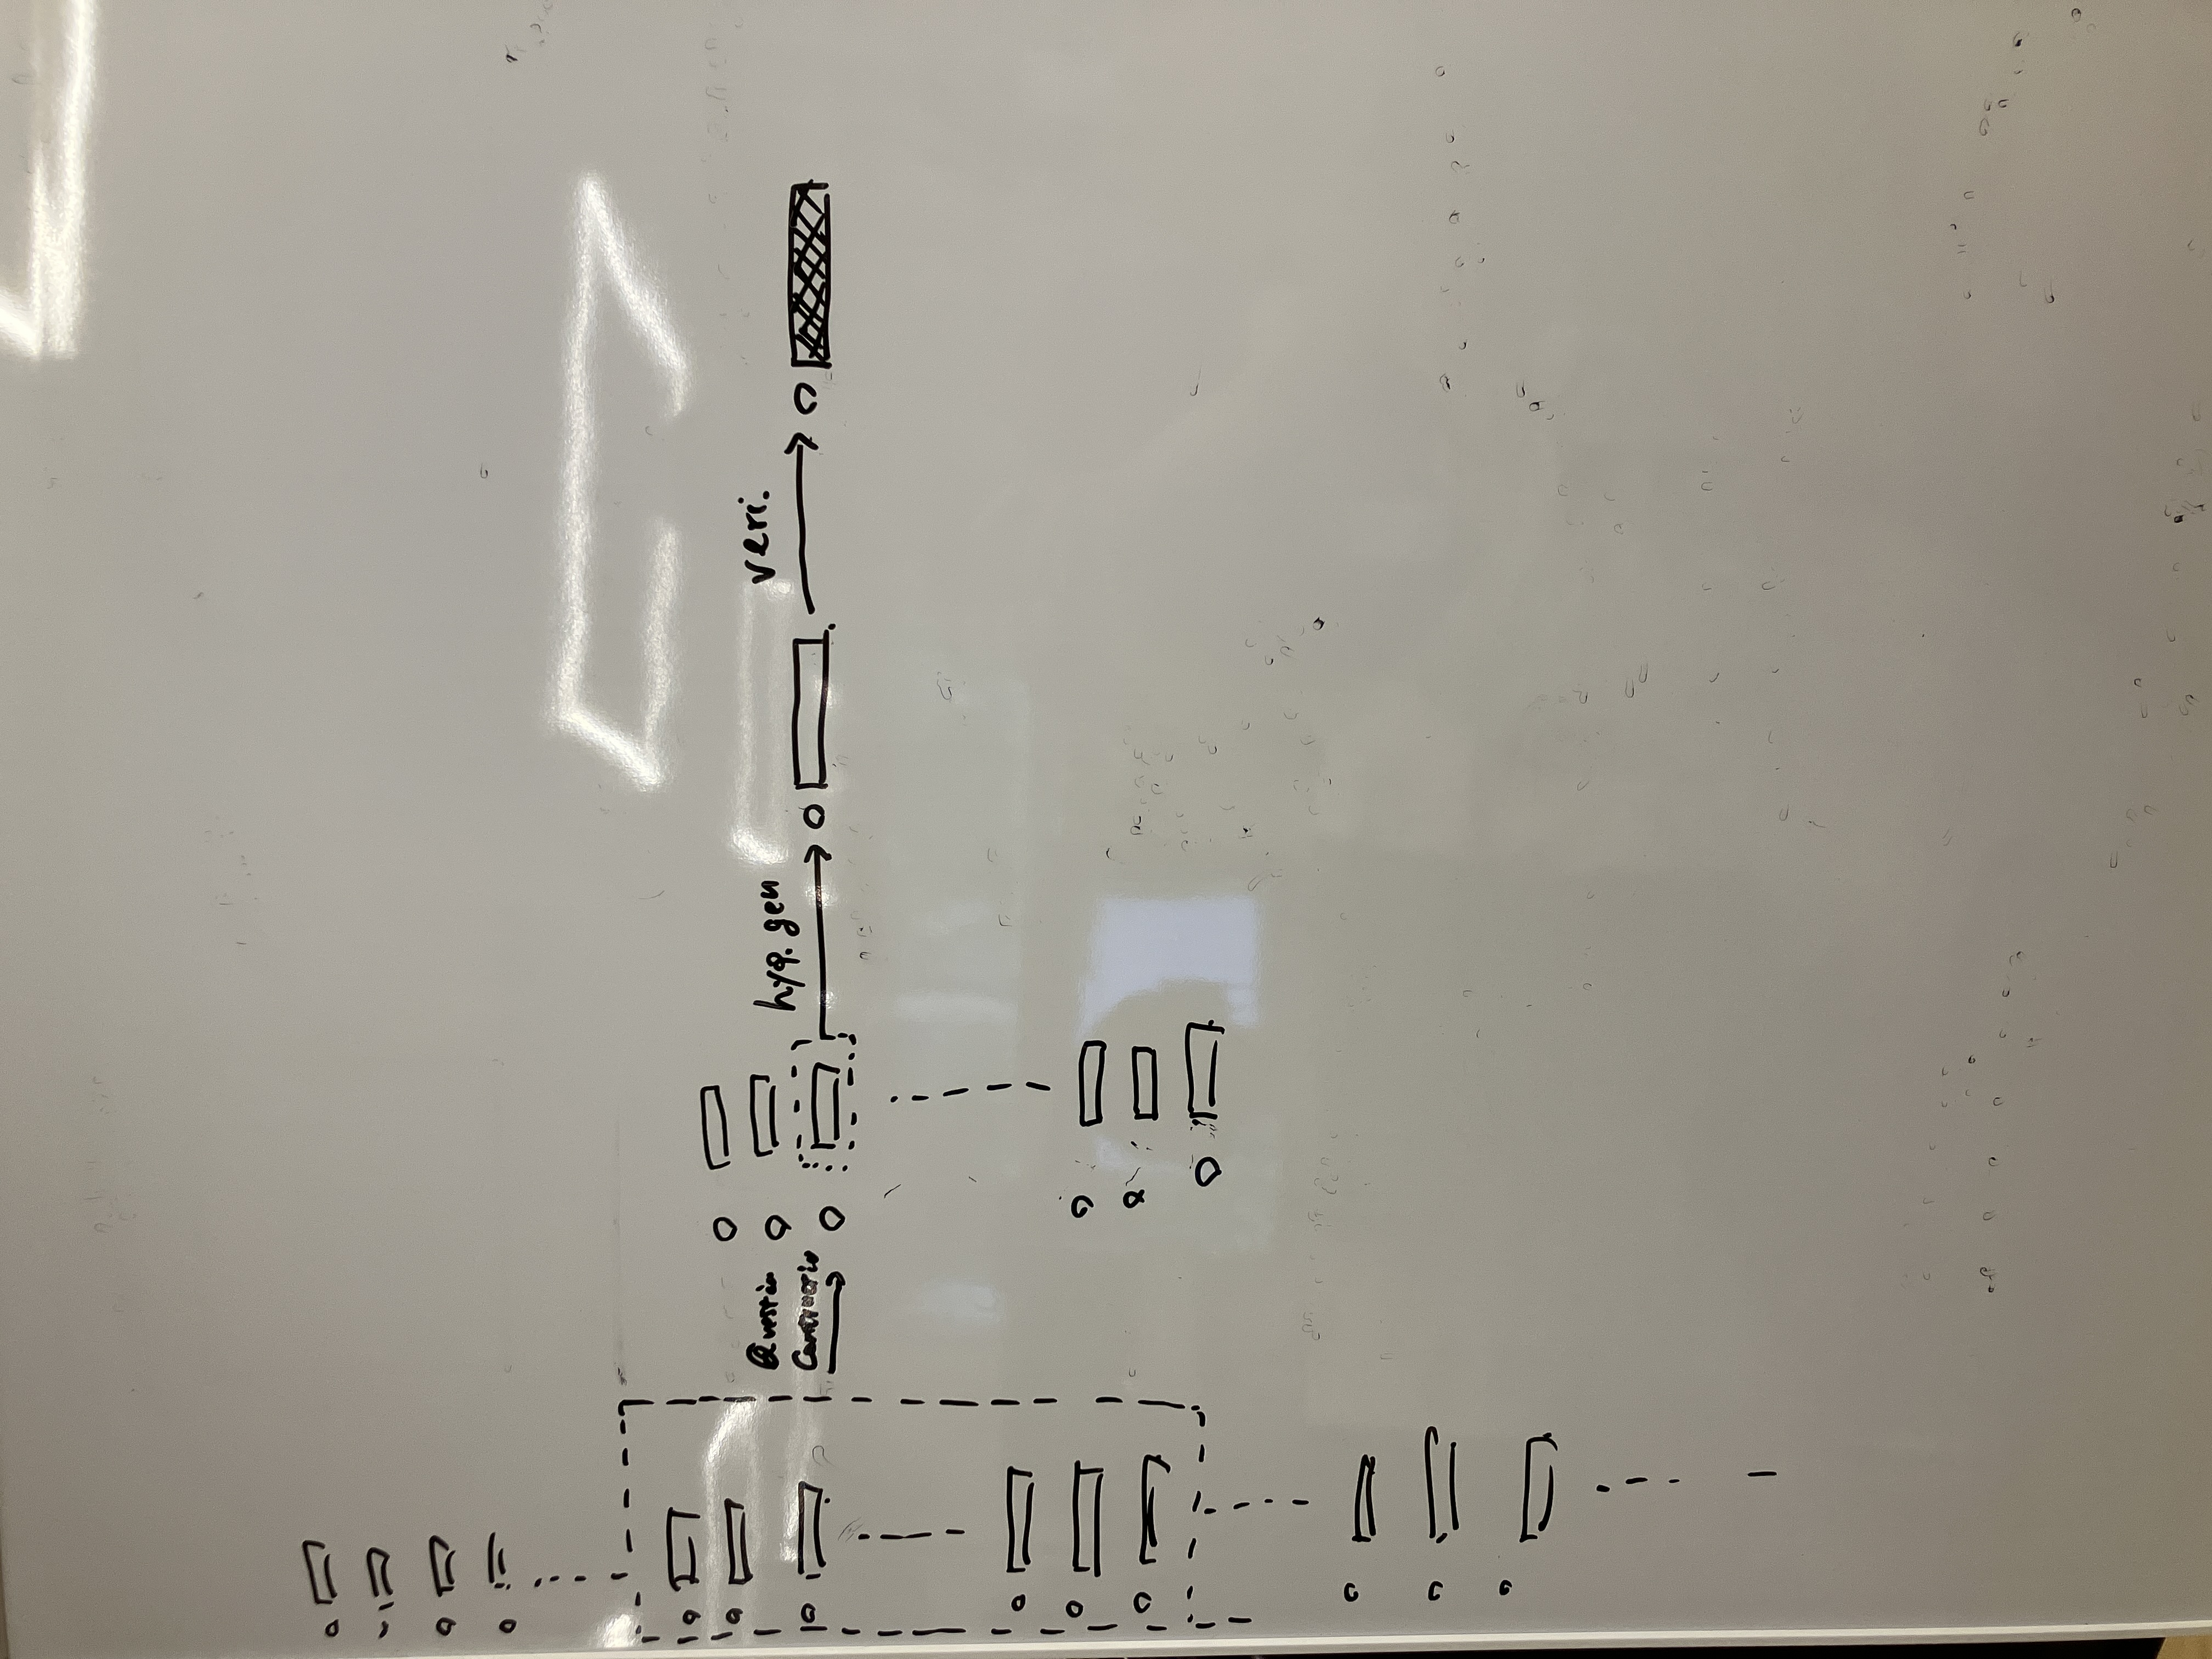
\includegraphics[width=\textwidth]{figs/beliefupdate.jpg}
    \caption{Research Process as Belief Update}
    \label{fig:beliefupdate}
\end{figure}
In the diagram, circles represent statements, and squares represent beliefs in response to those statements. Note that while circles were described as statements, they are not limited to textual representations as long as they are associated with beliefs. Beliefs are determined by the subject holding the belief (in this case, an agent) and the object of the belief (the statement), but please note that we are assuming a fixed agent in this context.

Firstly, in this world, there exist countless pairs of statements and corresponding beliefs (or latent beliefs). Posing a question corresponds to extracting a subset of unknown statements from this pool. More precisely, an unknown statement refers to a statement for which the agent is unsure whether to assign a strong or weak belief. Choosing corresponds to implicitly determining a function that assigns beliefs to each statement. For example, let's consider posing the question ``When did the universe begin?'' This answer to this question is unknown to humanity. By posing this question, the range of possible answers is narrowed down. However, it is not realistically possible for an agent to be aware of all statements and potential answers that could exist. Therefore, while we mentioned pairs of beliefs and statements, please consider that most of these beliefs are latent and potential.

Next, generating a hypothesis involves selecting one pair of a claim and a belief from among the potential claims that could serve as potential answers to the question. It is at this point, by choosing a hypothesis or considering multiple candidate hypotheses, that discourse becomes consciously acknowledged, and beliefs are substantively assigned. Finally, as we discussed in Chapter 2, verification involves gaining evidence for the belief in the chosen hypothesis, resulting in the updating of the belief state. The updated beliefs are represented in black in the diagram.

\chapter{Literature Review}
\label{chapter-literature-review}

\section{Pipeline}
While not necessarily using machine learning, there are several attempts to automate not a particular task but the entire research process. A seminal early works are Adam \cite{king2004functional}, and Eve \cite{williams2015cheaper}, closed-loop systems for scientific discovery. 

Additionally, the concept of a \textit{scientific workflow}, which represents data and computational processing pipelines in research as software, emerged in the early 2000s. The developments and advances in research related to scientific workflows are consolidated in this literature \cite{barker2008scientific,atkinson2017scientific}. Additionally, these papers \cite{deelman2019role,nouri2021exploring} discusses how machine learning contributes to streamline the each step in the scientific workflow.

These are not about creating machine learning agents that can do research. However, these are extremely important initiatives in terms of softwareizing the research process \cite{deelman2015pegasus,gil2011semantic}.

\section{Literacy}

\subsection{Searching}

Firstly, let us mention academic search engines that provide features to help researchers find relevant papers from a vast amount of literature \cite{googlescholar,semanticscholar,dblp,pubmed,citeseerx}. 

Specialized search systems have also been proposed for specific purposes. For example, some studies have been proposed systems to discover studis in other domeins \cite{kang2022augmenting}, difficulties, limitations and emerging hypotheses \cite{lahav2022search}, and author homepages \cite{patel2021author}. Also, in response to the COVID pandemic, several systems have emerged in recent times to search for COVID-19 related papers \cite{hope2020scisight}.

Instead of searching for papers manually, there are approaches that directly recommend papers to researchers. In practice, it is common for the specific aspects of academic papers that researchers want to compare to vary depending on the situation and research field. Therefore, researchers have invented the method allowing comparison in certain aspect of papers \cite{ostendorff2020aspect} and tailored to some particular research area \cite{breitinger2022recommending}. Also, some researchers study recommendation of authors instead of papers \cite{portenoy2022bursting}. A comprehensive summary of classical research on paper recommendation can be found in \cite{bai2019scientific}.

\subsection{Reading}
The majority of research on automation in research pertains to automating operations related to papers. Specifically, research on information extraction from papers constitutes the majority. Here, \textit{reading} refers to extracting information from a paper.

Several methods specialized in extracting specific information have been proposed. For instance, there are studies for extracting mathematical expressions \cite{greiner2020math,madisetty2021neural}, measure \cite{harper2021semeval,kohler2021s}, tabale and figure \cite{shen2022vila,hashmi2021current,zhuang2022resel,yamamoto2021visual}, dataset \cite{hou2019identification,kumar2021dataquest,prasad2019dataset}, and results \cite{kardas2020axcell}.

There are also studies that focus not on information extraction, but on determining the meaning of sentences written in papers. One representative example is research on citation classification, which involves understanding the intent behind the cited text \cite{pride2019act,kunnath2021meta,kunnath2022dynamic,kunnath2022act2,lauscher2021multicite}. Another example is topic/theme classification, which detect the main topic of the paper \cite{sadat2022hierarchical,mendoza2022benchmark,salatino2022cso}.

One of the most heavily researched areas of information extraction from scientific papers is summarization. Some studies propose methods to generate the contribution of a paper \cite{hayashi2020s}, scientific claims \cite{wright2022generating}, and lay summarization \cite{goldsack2022making}. Other studies have attempted to create better paper summaries using citation graph \cite{chen2022scientific,an2021enhancing}, or propose the summarization system \cite{erera2019summarization}.

Many of the earlier summarization studies only used limited information such as abstracts. In recent years, there have been proposed studies that generate summaries by reading the entire paper \cite{subramanian2019extractive,qi2022sapgraph,dong2020discourse,tretyak2020combination}.

Also, the number of papers has increased dramatically, and the time available for obtaining information from a single paper has become increasingly limited. Thus, some studies propose the methods to generate extremely short summaries, such as TLDR \cite{cachola2020tldr} and key phrases \cite{boudin2021keyphrase,garg2021keyphrase}.

To advance these summarization studies, some studies propose datasets \cite{yasunaga2019scisummnet,bastan2022sume} and annotation platforms \cite{el2022platform} for paper summarization. 

The early research on paper summarization, which was conducted relatively early, is well summarized in \cite{altmami2022automatic}. If you are interested, please also refer to this paper.

Up to this point, we have described methods that assume extracting specific information or summarizing papers. In contrast, there are studies that issue queries in natural language to retrieve desired information from papers. This has been formalized as a question-answering task, a more general problem setting \cite{lu2022learn,ruggeri2022argscichat,saikh2022scienceqa}. 

In the field of question-answering for academic papers, some web services have gained attention for its high performance \cite{elicit,scispace}. Elicit use large language models and compose them to write \textit{compositional language model programs}. Ought \cite{ought}, the provider of Elicit, publish the instructions of how to write compositional language model programs \cite{primer2022}. Also, they disclose how to update their system with their idea of \textit{process supervision} \cite{reppert2023iterated}. Therefore, for those who are interested in question-answering systems for scientific papers, we strongly recommend reading these papers and documents.

Lastly, many tools have been proposed to assist researchers in reading papers. These studies highlight rhetorical roles \cite{fok2023scim,lauscher2018arguminsci}, generate description to terminologies \cite{august2022generating,head2021augmenting,murthy2022accord}, simplify texts for non-experts \cite{august2022paper,jeblick2022chatgpt}, and allow interaction \cite{kang2022threddy,elicit,scispace}.

\subsection{Writing}
Research is the act of producing a novel knowledge on top of prior studies. The apt incorporation of previous literature and elucidation of the distinctions between the proposition and previous studies are essential. Consequently, some researchers have investigated to generate comparative arguments \cite{yu2022scientific} and others have studied to generate citation texts \cite{arita2022citation,gu2022controllable,wang2021autocite,xing2020automatic,funkquist2022citebench}. Additionally, several studies exist that, instead of directly producing text, aspire to assist in the writing process by recommending relevant literature for inclusion as citations \cite{farber2020citation,zhang2020dual,duma2019contextual,farber2018cite,gosangi2021use}. Furthermore, there exist investigations aimed at automating systematic reviews writing \cite{dones2022systematic}.

Scholarly articles are structured documents. This structural property enables researchers to generate texts per sections. Thereafter, 
researchers have endeavored to generate, for example, abstract \cite{kumarasinghe2022automatic,gao2022comparing,wang2019paperrobot}, related works \cite{li2022automatic,shah2021generating}, table description in result section \cite{moosavi2021scigen,moosavi2021learning}, conclusion, and future work \cite{wang2019paperrobot}. Wang et al. propose to generate even next research's probable title \cite{wang2019paperrobot}.

Similar to the situation with reading, proposals have emerged for systems to support writing \cite{narimatsu2021task}, as well as for datasets to train text generation \cite{chen2021scixgen}. In recent times, some researchers try to have GPT series to write academic papers \cite{transformer2022can}. 

\subsection{Scientific Language Models}

Whether engaging in reading or writing, the presence of a system that comprehends natural language is indispensable. In recent years, large-scale language models, trained on extensive textual data, have achieved significant success. Concurrently, numerous language models, specifically tailored to scientific documents, have also been proposed \cite{beltagy2019scibert,singh2022scirepeval,nadkarni2021scientific,cohan2020specter,gupta2022matscibert,taylor2022galactica}.

\section{Knowledge Production}
% The Process of Creating New Knowledge

% Modern research is constructed from three main phases: observation, hypothesis generation, and hypothesis validation <- not line but cycle

\subsection{Issue Discovery}
Lahav et al. have proposed a methodology for automating the discovery of prevailing challenges within the research community, as well as the emerging hypotheses to address them \cite{lahav2022search}.

\subsection{Hypothesis Generation}
A hypothesis is a proposition put forward in response to the problem or question that the research is focused on. These claims or proposals will be evaluated for their validity at a later stage through some form of procedure. These claims or proposals that involve uncertainty regarding its validity as an answer to the research objective are referred to as hypotheses in this context.

Because of its nature as an answer to the objective, what constitutes a hypothesis varies depending on the purpose of the research. For example, if a paper aims to enhance our understanding of a particular phenomenon, then the description or mechanism of that phenomenon would become the hypothesis. Similarly, if the objective is to solve a particular problem, then the solution to that problem would be considered the hypothesis. 

Therefore, we acknowledge that there are still few proposed methods for automatically generating hypotheses that are applicable to all research areas. However, there are already several attempts at automating the elements that are considered important in hypothesis generation.

\subsubsection{Analogy} 
% \subsubsection{Analogy} 
% TODO: Reframe this based on the cognitive aspect borrowing from "A Computational Inflection for Scientific Discovery"

One of the elements considered important in this regard is the automation of \textit{analogical reasoning}. While the specifics of the research objectives may differ, they all share a common aim of proposing solutions that transform the unknown into the known or unresolved into the resolved. However, it is impossible to make meaningful inferences about completely unrelated subjects that have no connection to the known. The objectives and potential proposals are expected to be similar to some extent to those that existed in the past. Therefore, discovering similarities in the structure of past objectives and the current objective, and applying the means that were effective in solving past problems to the new objective, can increase the likelihood of achieving the objective. In this sense, analogical reasoning, which involves inferences based on the structural similarities between two objects, is considered to be crucial for hypothesis generation \cite{hesse1965models,thagard_1984,gentner1993shift,holyoak1996mental,dunbar1997scientists,gentner2002analogy}. 

In recent years, several researchers have presented studies on automating scientific analogical reasoning for identifying the relationship between problems and their corresponding solutions using data from scientific papers \cite{kang2022augmenting,chan2018solvent}. 
Systems have been proposed that recommend researchers who are pursuing analogous objectives via divergent approaches \cite{portenoy2022bursting}. Similar to the case of analogical reasoning, this concentrates on abstract relationships, aiding in the generation of beneficial hypotheses by applying previously successful methods to novel techniques.

\subsubsection{Symbolic Regression} 

Modern science is composed of a cycle of observation, hypothesis generation, and hypothesis testing. In many fields, including physics, chemistry, and biology, mathematical models are often constructed as hypotheses from observational data. That is to say, formulating a mathematical representation that elucidates the phenomenon behind the data is an extremely critical step in science. One attempt to automate this endeavor is symbolic regression \cite{makke2022interpretable}, or equation discovery. While classical approaches to symbolic regression have traditionally employed methods such as evolutionary computation, recent years have seen the emergence of strategies utilizing deep neural networks \cite{petersen2019deep,udrescu2020ai,udrescu2020ai2,cranmer2020discovering,kamienny2022end,d2022deep}. Some researchers have proposed the frameworks \cite{landajuela2022unified,keren2023computational} and benchmarks \cite{matsubara2022rethinking} for symbolic regression. You can find a literature review of symbolic regression in \cite{makke2022interpretable}, and that of the early studies in \cite{kramer2023automated}.

\subsubsection{Others} 

Indeed, some methods have been proposed that don't generate hypotheses directly, but rather assist humans in generating hypotheses from experimental data 
 \cite{friederich2021scientific}.

\subsection{Verification}
\subsubsection{Verification Design}

Once a hypothesis is formulated, a plan is developed to test its validity. The design of this verification plan is far more flexible than that of hypothesis generation, making it more difficult to handle uniformly. To be more precise, while many sciences have standardized methods such as statistical tests for verification, there is a wide variety of methods for generating the data used for the verification. One study may require a huge machine to collide elementary particles, while another may use rats for behavioral experiments. Some studies may require the use of chemicals, while others can be simulated on a computer. Furthermore, even with standardized statistical tests, as mentioned earlier, automating their creation from scratch proves exceedingly challenging. It is readily apparent that devising standardized methodologies like statistical tests is difficult when one must not merely employ them as tools but also contemplate the very nature of what it means to verify, as well as the rationale behind adopting specific assumptions. Therefore, it may not be an overstatement to say that this aspect represents the biggest obstacle towards achieving complete automation of research in a unified manner.

Some researchers have tried to automate experimental design for quantum physics \cite{ruiz2022digital} or proposed to design workflow of scientific research as a software \cite{goble2020fair}. Additionally, research exists that proposes machine learning algorithms for formulating and executing experimental designs in a more abstract and simple manner \cite{herrmann2022learning}. The field of \textit{experimental design} has a long-standing history. Its primary objective is the automation of appropriate configuration and exploration for various conditions after you designed a base structure of an experiment. Specifically, research involving techniques such as Bayesian optimization for condition search has been conducted for some time \cite{chaloner1995bayesian,shahriari2015taking}.

\subsubsection{Verification Execution}

Once a verification plan has been devised, the process proceeds in accordance with it. As previously mentioned, the approach may vary considerably. However, in many scientific methodologies, statistical techniques are employed. In these instances, the verification process can be broadly divided into two stages: 1. data generation and 2. analysis of the generated data for validation.

As previously mentioned, data generation methods span a wide range. Among these, attempts have been made to automate the work of researchers within laboratories, an endeavor known as Laboratory Automation. For instance, 
some studies focus on automating cell culture tasks using humanoid robots \cite{ochiai2021variable},
% TODO: add more

% TODO: may differentiate the analysis for hypothesis generation from that for verification
we interpret data processed according to a certain criterion, assessing the validity of our inferences. Here, we make an explicit distinction between analysis for verification and analysis for hypothesis generation. Modern science is composed of a cycle of observation, hypothesis generation, and hypothesis testing. It's common to generate the next hypothesis to be tested from data produced for verification. However, this merely signifies that we conduct both hypothesis generation and testing through a somewhat inductive reasoning based on data. Therefore, in this context, we will focus on data analysis for hypothesis testing, while data analysis for hypothesis generation will be included in the hypothesis generation section introduced earlier.

To validate the plausibility of assertions, we currently employ statistical methods. There is research that automate the hypothesis testing \cite{gil2016automated}. 

Some researchers have engaged on automating data visualization and analysis \cite{bavishi2021vizsmith,bavishi2022tools}



\subsection{Peer Review}
Many studies have tried to automate peer review generation \cite{thelwall2019artificial,li2019generating,schulz2022future,yuan2022can,yuan2022kid,lin2021automated1,lin2021automated2,kumar2022investigations,bharti2022can,uban2021generating,wang2020reviewrobot}. While not generating peer reviews directly, studies focused on automating research paper assessment  can be said to be related to the peer review automation. \cite{kousha2022artificial,li2020multi,huang2018deep}. These studies have proposed the method to assess the quality \cite{thelwall2022predicting,thelwall2022can}, novelty \cite{pelletier2022novelpy,amplayo2019evaluating,shibayama2020measuring}, soundness \cite{cabanac2022decontamination}, and significance \cite{zong2022citation,xia2023review,soni2022predicting,manghi2021new,soni2021follow,van2020schubert,mckeown2016predicting}.

These investigations concern the automation of processes occurring subsequent to a manuscript's arrival at the hands of reviewers. Conversely, researchers also have investigated the automation before that process, such as determining the appropriate journal for submission \cite{michail2023journal} and assigning the reviewers \cite{zhao2022reviewer}.

While not centered on automation, certain studies engage in the scientific analysis of the review process \cite{shah2022challenges,verma2021attend,bharti2022confident,bharti2022betterpr,verma2022lack,kennard2022disapere}. These investigations serve to enhance our understanding of the nature of peer review and, in turn, provide valuable insights for the design of more effective automated review methodologies. Furthermore, automating the \textit{scientific claim verification} \cite{li2019scientific,wadden2020fact,wadden2022scifact,wadden2022multivers}, which determines the validity of a scientific claim through analysis of research paper corpora, is likely to contribute to the automation of the peer-review process.

\section{Knowledge Sharing}

Upon the completion of a study, the drafting of a manuscript, and its successful navigation of the peer-review process, the resulting findings are deemed to possess a degree of credibility as knowledge. Naturally, it would be hasty to assert that this alone births "correct" knowledge, as research demands iterative verification to confirm its validity. We convey such knowledge to others through various means, one of which is the presentation of research findings. To effectively communicate these outcomes, we create slides that elucidate our work. Studies also exist that strive to automate this aspect of the dissemination process \cite{sefid2019automatic}.

\section{Perspectives}

Gill presents an extremely exciting idea of conducting automated research by turning the entire scientific process into compositional and modular software with the literature review of her and her colleagues' work. \cite{gil2022will}. For example, Gill et al. have created a software of the semantic workflow of scientific data analysis and computation process  \cite{gil2011semantic}. 
Each step of this workflow modularizes the procedures in research. Not only can these make analysis more efficient, but they also allow for the analysis of the research process itself. Furthermore, common workflows can be identified from multiple workflows, enabling abstraction of cross-domain knowledge about research process. Additionally, Gill and her team have proposed DISK, a systematic framework for hypothesis testing and data analysis. DISK can automatically cycle through a series of processes, including the generation of hypotheses, the determination of data and methods to test them, the acquisition of data from shared repositories, the analysis of that data, and the modification of hypotheses. Furthermore, each hypothesis is associated with information on confidence level and analysis details, which significantly indicates the plausibility of the hypothesis. Additionally, as the hypothesis and its confidence level and analysis are continuously updated and the revision history is retained, it enables the continuous maintenance and update of scientific findings.

Kitano also harbors an ambition to automate the entirety of the research process \cite{kitano2021nobel}. This is a thought-provoking paper that is meticulously contemplated. Kitano underscores the ability of AI in automating science to execute exhaustive and thorough exploration as a significant strength. We, as humans, aim to generate hypotheses that yield impactful results (Kitano refers to this as a value-driven approach). However, the importance of research findings is context-dependent, and research that we humans deemed unimportant may become crucial if the presuppositions or the context alter. Kitano proposes to eschew this value-driven approach and implement an alternative, exploration-driven methodology to science, aiming for novel scientific discoveries that were unattainable by human capabilities. Besides, Kitano with many examples and detailed consideration, presents a plethora of stimulating ideas, such as the continuous hypothesis network update, a roadmap to achieve autonomous artificial scientists, and proposition of the Nobel Turing Challenge as a Grand Challenge to substantially advance these endeavors. We highly encourage those interested to delve into this fascinating read.

Hope et al. have written a captivating perspective paper on the automation of research, presenting a fresh and exciting viewpoint \cite{hope2022computational}. They introduce a human-centric idea aimed at efficiently extracting relevant information from the ever-expanding body of research data, tailored specifically to the tasks researchers are engaged in - a framework they term \textit{task-guided scientific knowledge retrieval}. They start by conceptualizing the act of research as an interaction between a researcher's \textit{inner cognitive world} and the \textit{outer world}, or \textit{scientific ecosystem}. Building on this, they underscore the vital role of representing and retrieving information that aligns with the inner cognitive world of researchers, deftly transforming the cognitive functions used in human research into algorithmic processes.

Extensive discourse transpires concerning scientific discoveries. Yet, discussions pertaining to scientific comprehension remain relatively unexplored. Hope et al. delve into the conundrum of what it entails for a machine learning agent to not only unearth scientific knowledge but also to comprehend it \cite{krenn2022scientific}. They adopt a human-centric stance, positing that an agent's ability to offer explanations comprehensible to human scientists signifies the existence of its scientific understanding.

\section{Applications}

\subsection{Mathematics}
The automation of mathematical proof, \textit{automated theorem proving} (ATP) , has been studied for a long tius. Recently several effort has come up to improve ATP by using machine learning, and especially deep learning. The 
 early seminal work is led by Schulz \cite{schulz2001learning} and Urban \cite{urban2004mptp,urban2008malarea}. The first work applying deep learning to ATP is \cite{irving2016deepmath}. Subsequently, numerous studies have emerged on Automated Theorem Proving (ATP) using deep learning \cite{bansal2019holist}. Recent studies on this topic are well organized in the following paper, so we recommend reading it if interested \cite{rabe2021towards}.
 % TODO: more organized literature review

 While research has been accumulated on ATP, there is still not much research done on the automated theorem discovery with a few exceptions \cite{gao2014systematic}. In recent years, attempts have been made to help humans to find mathematical conjectures \cite{davies2021advancing} and
 automatically generate mathematical conjectures \cite{raayoni2021generating}  using machine learning.

\subsection{Science}


It has become commonplace to streamline domain-specific tasks in scientific research using machine learning, resulting in a vast number of published papers. Even just to mention a few that come to mind, there are studies on molecular biology \cite{jumper2021highly,senior2020improved}, material science \cite{ramprasad2017machine}, medical science \cite{vamathevan2019applications,shorten2021deep}, quantum mechanics \cite{carleo2017solving}, cosmology \cite{carleo2019machine}, genetics \cite{libbrecht2015machine}, and nuclear physics \cite{degrave2022magnetic}. It is impossible to cover all of these applied studies of research automation of science. Therefore, in this paper, we will not go into detail about each of these studies. Instead, we will present research on automation of elements that can be applied in various fields of science. For the literature survey of domain specific automation, please refer to \cite{xu2021artificial}. \textcolor{red}{TODO: Add application studies}



\chapter{Proposal}
\label{chapter-proposal}
In this chapter, we will discuss what should be done and how to achieve the realization of autonomous artificial researchers. Firstly, we will provide an overview of Chapter 1 and Chapter 2. Building upon that, we will propose sub-goals to aim for in order to achieve autonomous artificial researchers. Subsequently, for each sub-goal, we will organize subtasks and propose a general approach and strategy for how to pursue these intermediate goals.

As we have reiterated multiple times, the ultimate goal is to create an artificial intelligence that can autonomously conduct research. Therefore, in order to clarify the objectives, it is necessary to define what it means for an AI to be able to conduct research and what it means for it to be autonomous. Let's first discuss these aspects.

\section{Bootstrapping}
Do research automation that contribute to research automation research.

\section{Goal}
To reiterate, the proposition put forward in this paper is to strive for the realization of autonomous intelligent systems that can conduct research. This is because I believe it holds the potential to liberate research from the cognitive, historical, and social constraints that surround humans. Furthermore, I think it can lead to a future where better knowledge production occurs, ultimately enabling a broader and deeper understanding of the universe and nature.

I believe that more people should engage in efforts aimed at developing artificial intelligence that autonomously conducts research on universal subjects. This is because there currently seems to be a limited number of such endeavors. Firstly, I think efforts in research automation can be classified along the axes of universality and autonomy. Universality refers to how many research fields a single automated research system can handle. For example, a system capable of conducting research in both physics and history would have higher universality compared to a system limited to either one. This can be understood as the ability to tackle universal questions. Next, autonomy refers to the level of human intervention involved. For instance, a system that requires humans to explicitly provide a set of hypotheses has lower autonomy compared to one that allows the machine to discover them on its own. From this perspective, previous endeavors in research automation can be organized as illustrated in the following diagram. (Diagram description). Thus, it can be said that there are still relatively few efforts focused on constructing highly universal and autonomous automated research systems.

\textcolor{red}{TODO: Add Fig}

Of course, efforts to automate research at all levels are important. For example, initiatives to automate a specific experiment in physics are valuable in their own right, as they aim to achieve the specific objective of enabling more efficient research. Therefore, the endeavors mentioned in this paper differ in their original goals, and it is not a matter of determining which is better or more important. Additionally, insights gained from these endeavors related to the construction of highly universal and autonomous systems are crucial. As achieving such systems involves high uncertainty, it is beneficial to start by creating concrete systems to increase problem resolution. This process will involve considering which aspects of a specific system can be abstracted to achieve universality and autonomy. Hence, the most important aspect is that all initiatives aspiring towards research automation gain momentum.

\subsection{Goal and Research}
First, let's discuss what it means for an AI to be able to conduct research. We delved into this topic in detail in Chapter 2. Research is the act of producing new knowledge for a community of constituents capable of forming shared beliefs. Producing new knowledge involves posing unanswered questions, formulating hypotheses in response to those questions, and verifying those hypotheses to update beliefs. Therefore, creating an intelligent system capable of conducting research means creating a system that can perform these tasks.

\textcolor{red}{TODO: revision}

\subsection{Goal and Autonomy}
% The ultimate goal is to create an artificial intelligence that can produce knowledge. In other words, the aim is to develop a function that can autonomously generate some form of knowledge when given any input. Therefore, any attempt to achieve the realization of an artificial researcher should strive to create such a function, regardless of its specific form. As we have reiterated, if the knowledge generated through research is a shared belief in a justified and true society, then the goal can be rephrased as aiming to generate a belief in response to any input and justify it to the extent that it becomes a shared belief in a society.

What we are aiming for is an artificial intelligence that can conduct research completely autonomously. Therefore, the ultimate aim is to minimize predetermined modules or algorithms decided by humans and create an end-to-end system. With that in mind, we would like to express our opinion on how much autonomy should be pursued.

Firstly, autonomy ultimately boils down to the question of how much is taken for granted. The more predetermined elements there are, the lower the autonomy, and the fewer predetermined elements there are, the higher the autonomy. In this sense, autonomy is continuous and incremental.

The highest level of autonomy in pursuing the realization of an artificial researcher is a state where the system invents and conducts research without assuming its purpose is knowledge production. This means not instructing the system to conduct research, not teaching what research is beforehand, but enabling the acquisition and execution of research. Humans can be considered researchers with this level of autonomy at least at the species level. This is because while humans are probably not designed as systems dedicated solely to research, they have progressively invented research throughout history. Of course, such a level of autonomy is not achievable without any assumptions, so if one aims for this level of autonomy, it is necessary to prepare an environment that induces the acquisition of research and design some form of inductive bias. What we are referring to here is a system with autonomy in the sense that research is acquired as a result of computational processing indirectly related to knowledge production and the necessary conditions for it.

However, demanding such a level of autonomy may be somewhat excessive when it comes to pursuing an autonomous artificial researcher. Therefore, it seems reasonable to assume knowledge production as a design requirement. Since knowledge production is assumed, some form of information about what knowledge is must be provided. Here, we can classify it into two categories.

The first is implicitly providing information about what research is. This involves allowing the system to acquire the concept of research on its own based on existing knowledge and data about the process of generating hypotheses and methods of verification. The history of machine learning research has shown the power of this end-to-end direction in creating strong intelligent systems. In that sense, this direction can be considered one of the directions to pursue.

The second is explicitly providing information about what research is. This involves providing only the necessary information about the conditions related to research and aiming for their fulfillment. It does not mean explicitly instructing how to construct questions or specific means to justify beliefs. Instead, it only provides information about what needs to be done, and the system must acquire and execute them on its own. This is autonomy in the sense that one must acquire the methods oneself and execute them. We believe that if we provide information at this level, it can be considered a system capable of conducting research autonomously. On the other hand, we think that research achieved by hard-coding the processing within the construction of questions, hypothesis generation, and verification, while automatic, is not autonomous.

While achieving the autonomy in the first two stages would certainly be great, it is expected to be quite challenging to aim for that directly. Therefore, we believe it is better to aim for the third level of autonomy. Specifically, as proposed in Chapter 2, it would be beneficial to aim to create a system that divides the research process into three modules: question construction, hypothesis generation, and verification, and connects them as a pipeline. To achieve that system, we should strive to incrementally enhance the internal autonomy of each module.

\textcolor{red}{TODO: revision}

\section{What to Do to Achieve the Objective}

To create a universal artificial researcher, I believe it is necessary to automate the construction of questions, generation of hypotheses, and validation of hypotheses. This is because, as seen in Chapter 1, these functions appear to be essential in all research. In other words, by automating these functions as much as possible without relying on human intervention, we can move closer to the realization of an autonomous and universal artificial researcher.

% \subsection{question construction}
% The construction of a question is the act of seeking information \cite{watson2015ask}. Specifically, in the context of research, we consider information as knowledge. The act of seeking knowledge involves two steps: 1. Recognizing the lack of knowledge and 2. Attempting to fill that knowledge gap. In this discussion, we assume that intelligence is designed to consistently generate questions when given input. Therefore, we temporarily set aside the aspect of "triggering action" related to the second step of attempting to fill the knowledge gap.

% The recognition of a knowledge gap occurs when we expect to have certain knowledge and, upon referencing our accessible knowledge, we find that it is not available. For example, when running a program and encountering an error that we cannot resolve on our own, we recognize that we lack the necessary knowledge.

% The reasons for expecting the existence of certain knowledge can vary and are arbitrary. In this case, we assume that a purpose given by a third party creates an expectation of certain knowledge. For example, in the case of humans, we first consider what we need to do to achieve a certain purpose. We then anticipate the necessary knowledge to accomplish those tasks, and when we find that it is not present within our existing knowledge, we recognize the knowledge gap.

% Lastly, in this discussion, knowledge refers to the collective body of research findings, particularly academic papers. In actual research, a researcher may personally have a question and then investigate previous studies to confirm that it is indeed unknown before formulating it as a research question. However, what is important in the construction of a research question is that it is unknown to other entities. Therefore, for simplicity, we directly refer to the entirety of academic papers without including the step of comparing personal knowledge.

% To summarize, to create an intelligence capable of constructing questions in this setting, we need to design it to expect the necessary knowledge to achieve a given purpose provided by a third party, search for that knowledge in academic papers, assess whether the papers contain sufficient knowledge to achieve the purpose, and express any knowledge gaps as questions.

% In this case, we excluded the discussion of triggering action by design. However, when considering increasing autonomy, it is important to discuss how to incorporate this aspect into learning and acquisition. The question of "why do we seek information" has been extensively discussed in the context of curiosity.

% Furthermore, in this case, we defined the expectation of knowledge as aiming to achieve a given purpose. However, as mentioned earlier, this does not affect the formulation of questions. For example, let's consider the case of a child asking, ``Why is the sky blue?'' In this case, the child may already have prior knowledge of the concept of ``sky'' and ``blue.'' Additionally, they may possess a naive concept of causality, believing that ``A is B, so there must be a reason for it.'' Thus, they may have expected to have the knowledge that ``the sky is blue because of B.'' However, when they reference their internal knowledge, they find that it does not contain the corresponding knowledge. Therefore, they may have asked the question ``Why is the sky blue?'' to evoke the knowledge they were lacking.

% In this way, the reasons for expecting the existence of certain knowledge can vary, and what, why, and how we seek information (knowledge) are not constrained by specific conditions. Therefore, when attempting to create an intelligence capable of constructing questions in the future, it is feasible to develop a more flexible intelligence.

% Additionally, in this case, we assumed that the given purpose and its achievement are predefined goals. However, humans naturally set their own goals. When considering the design of a more autonomous intelligence, it is conceivable to aim for automation in this aspect as well. However, as mentioned earlier, the question of what we seek knowledge about is not specific to research. Therefore

% , we temporarily set it aside for now. If we were to pursue this direction further, it would ultimately lead to an infinite regress, raising the question of how much information to consider as given.

% \begin{figure}[htb]
%     \centering
%     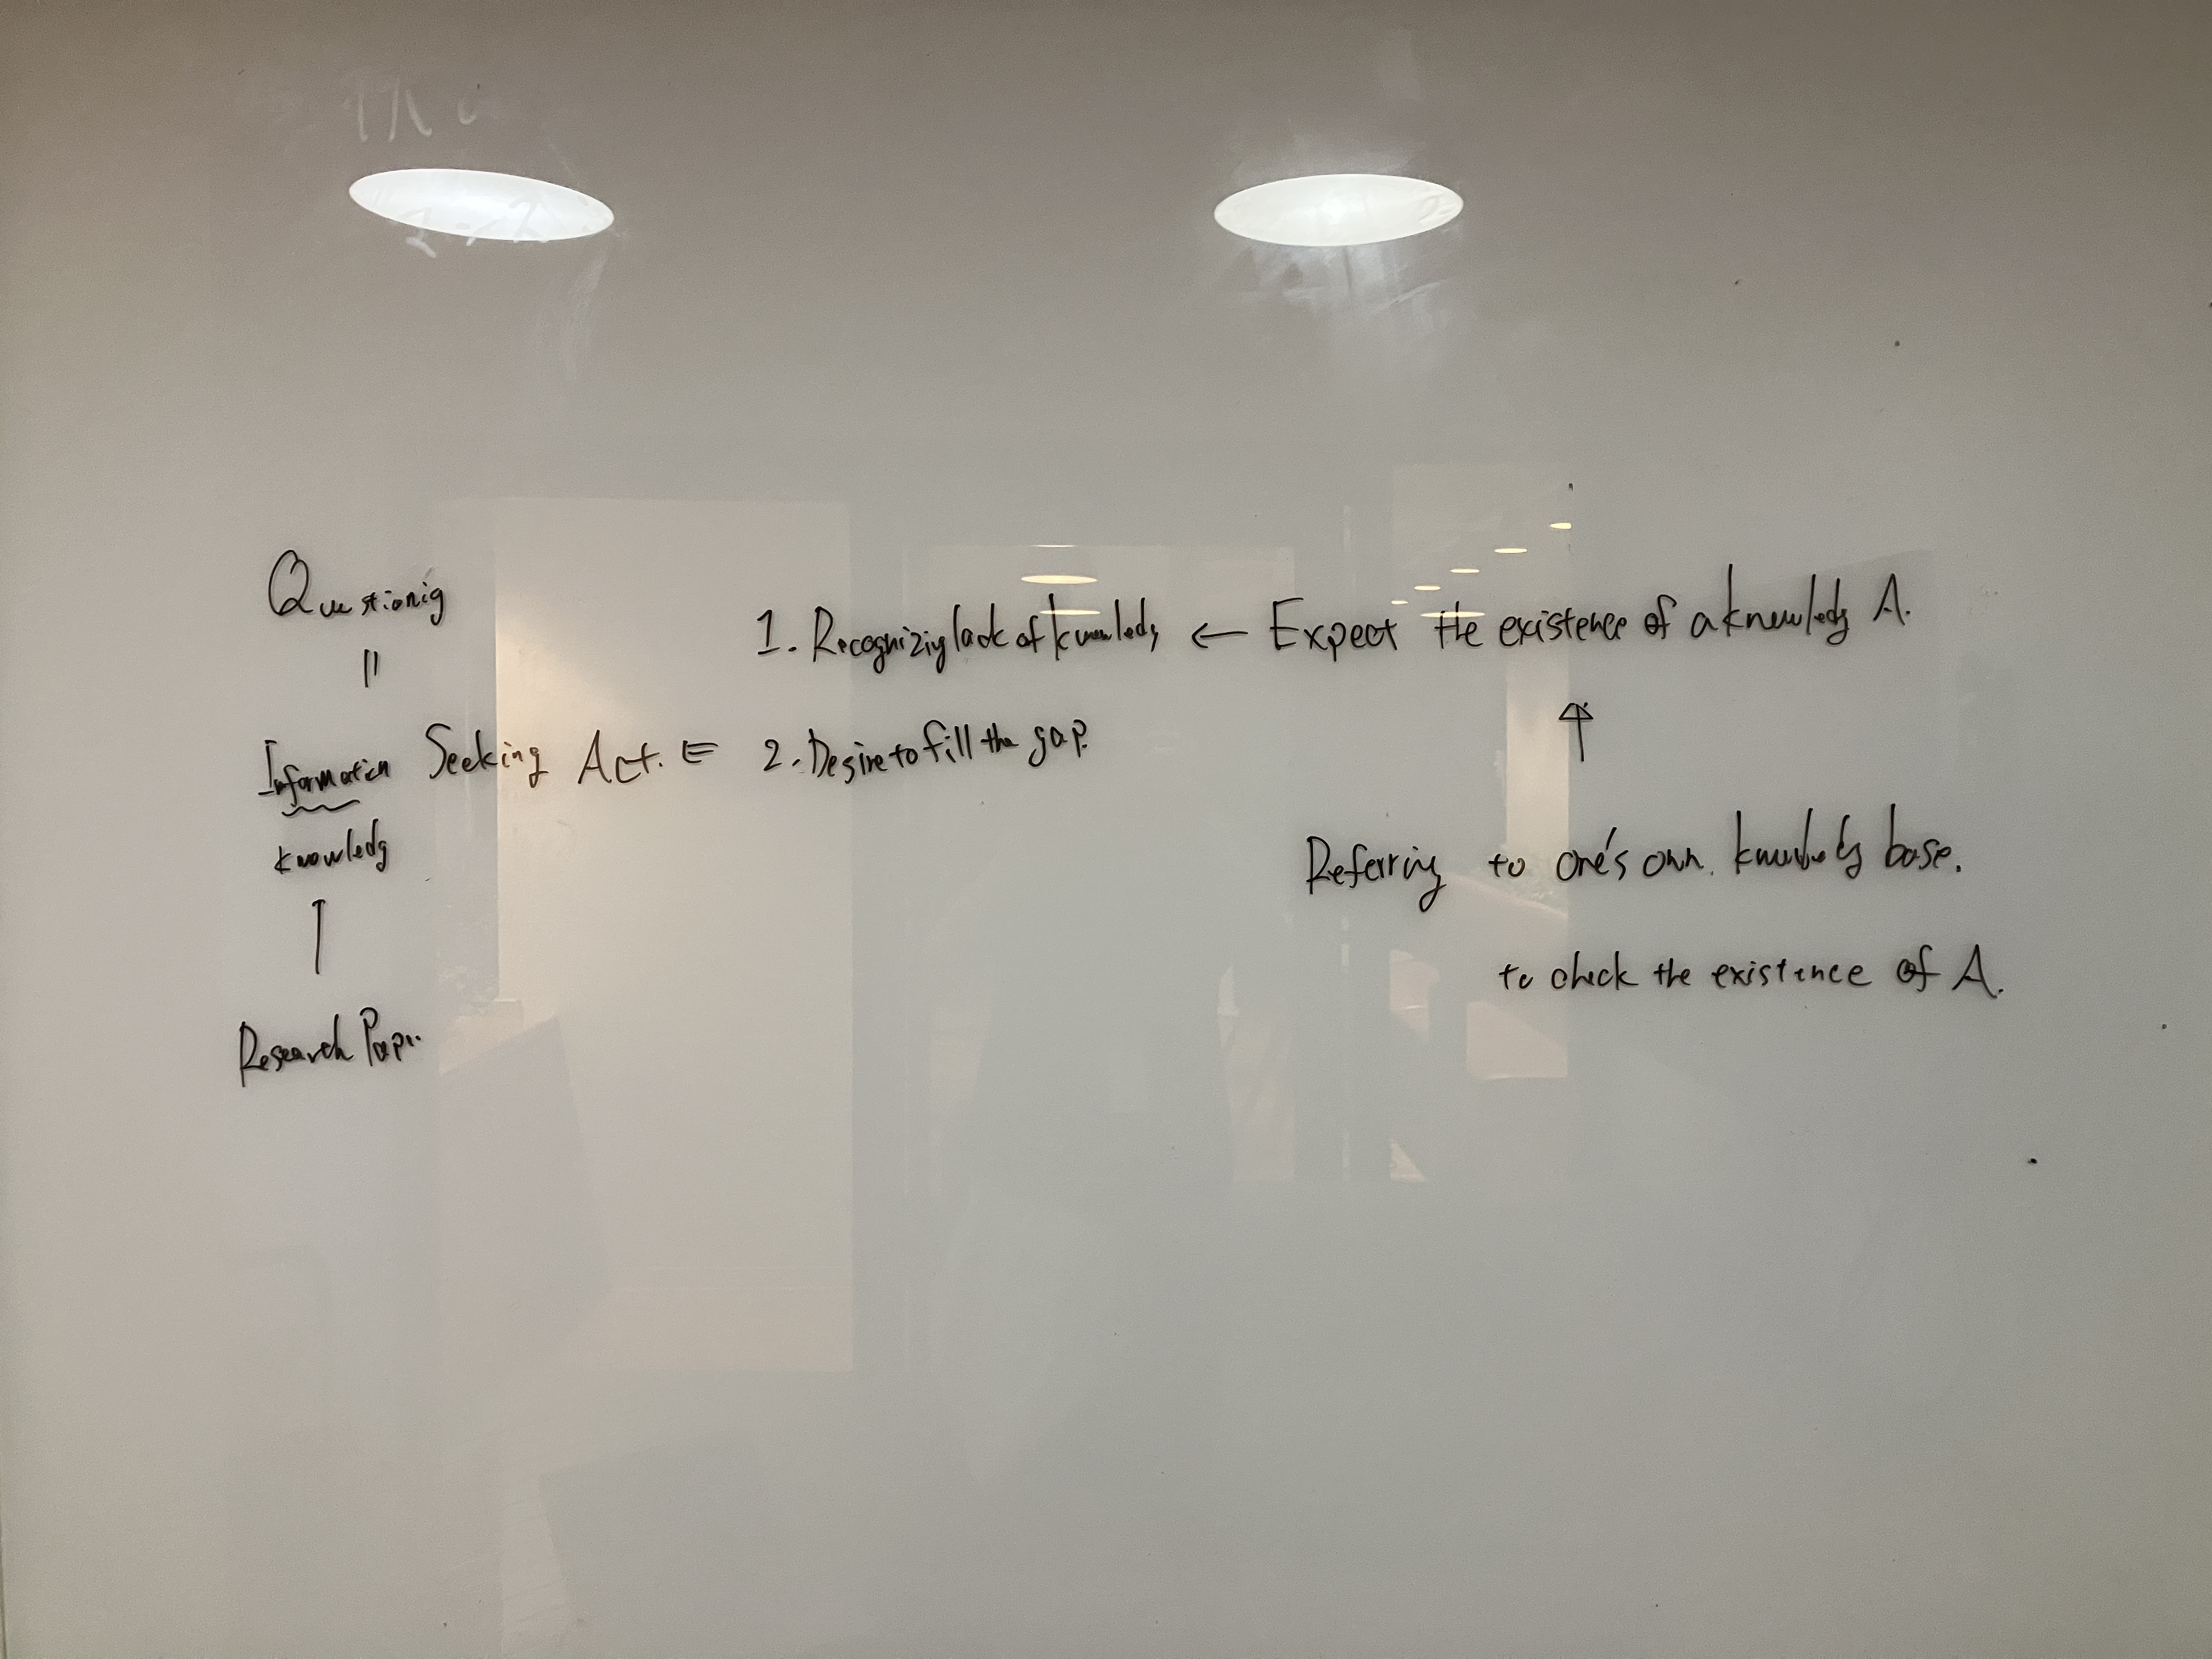
\includegraphics[width=\textwidth]{figs/question_formulation.jpg}
%     \caption{question construction}
%     \label{fig:enter-label}
% \end{figure}

% \subsubsection{How to Identify the Necessary Knowledge for Achieving a Goal?}
% In this situation, we need to consider how to identify the knowledge required to achieve our objectives. Typically, when given a goal, we start by listing the necessary elements to accomplish it. For example, to achieve general artificial intelligence, we may think that it requires the ability to handle language, understand the real world, be proficient in mathematics, and align with human values. To understand the real world, for instance, we may need the capability for interacting with the physical world, processing visual information, and so on. These requirements can be further broken down into multiple necessary elements. By repeating this process, we can narrow down the specific tasks that can be directly addressed. Then, the required knowledge to accomplish those tasks is demanded, and that's where it directly connects to the research question.

% Several things are happening here. Firstly, listing the elements necessary for achieving the goal means generating sub-goals from the main goal. However, it's always a challenging problem to evaluate how a particular sub-goal contributes to the achievement of a given goal. Especially in the case of research, the target might be an too general and ambitious vision that nobody has achieved before, so we need to think about what needs to be done to break it down into appropriate sub-problems. In other words, it is necessary to construct a tree with nodes representing sub-goals.

% Secondly, it is necessary to identify the most important sub-goal from the selected candidate sub-goals. Since only one question can be addressed in the end, it is necessary to select a single sub-goal using some evaluation criteria. This may not be a problem if the sub-goals can be judged on the same evaluation criteria, but in many cases, unrelated sub-goals may arise. For example, to create general artificial intelligence, the development of machine learning theory may be equally important as the advancement of semiconductor technology. However, it may be difficult to compare their importance on the same evaluation axis.

% Thirdly, the question to ultimately arrive at must be verifiable. If the question is not specific, meaningful verification cannot be performed. Overly broad or ambiguous questions can result in countless or trivial answers, or they may be too unclear to provide practical answers. Increasing the specificity of the question corresponds to deepening the depth of the sub-goal tree, so it may be important to construct a sufficiently deep tree and find an efficient way to navigate it. The verifiability is constrained by the knowledge, resources, such as funding and technology, that we currently have. Therefore, when conducting verification in reality, it is necessary to consider such feasibility. Whether to tackle a question with high feasibility or to further divide it into more subtasks for its realization is a matter of judgment. In any case, it is necessary to appropriately evaluate such feasibility. The scope of feasibility is vast, so it is a challenging problem to determine how to consider it in creating intelligent systems.

% Here, we discussed what needs to be done to construct questions that generate the necessary knowledge to achieve the goal. We believe that research that can generate knowledge that is expected to contribute to the achievement of the goal, and that has not been revealed in previous studies, can be considered as ``important'' research. In that sense, it may be important to consider how to achieve the automation of research in this direction.

% In this discussion, we have only touched upon a limited number of points that we personally consider important. However, we believe that there are other important points that should be considered. By seriously reflecting on ``how questions are currently being constructed,'' these points are expected to become clearer.

% Also, in this discussion, we considered the method of outputting questions from the goal through the construction and exploration of a tree structure. However, as mentioned by the predecessors, if an end-to-end approach ultimately becomes a powerful method, it may be more desirable to consider a direction in which questions are directly output from the goal. In particular, even when performing multi-step reasoning, it seems more natural to improve reasoning abilities using the recently developed approaches to multi-step logical reasoning, rather than explicitly considering tree structures. While the development of methods for multi-step reasoning is undoubtedly important in pursuing this direction, this is not a point that needs to be emphasized here as it is being addressed not only in the context of research automation but also more generally. As a discussion focused on the automation of research, it may be worth considering the construction of higher-quality datasets for goals and research questions. For example, it may be possible to construct a dataset by extracting only the ultimate goal and the research questions actually solved from the introductions of papers.

% However, an important point to note here is that the research questions created by humans so far are not necessarily optimal for achieving research goals. Firstly, machines may be capable of maximizing the objective better than humans due to cognitive constraints. Secondly, not all human research has been conducted by working backward from a clear goal. Some studies were conducted simply because they seemed interesting while reading papers. Additionally, as mentioned earlier, abstraction has significantly advanced science, but there are cases where the study of abstraction itself is the

%  objective rather than abstraction in some specific cases. In this regard, simply learning from human data without imitation may constrain the potential capabilities that machines can possess. Therefore, it becomes important to consider how to formulate the maximization of the probability of achieving research goals as a problem, rather than naive learning from human data.

% \subsubsection{How to Search Necessary Knowledge and Recognize the Lack of Knowledge?}
% There are various methods to determine whether the desired knowledge already exists. Typically, it is considered that candidates can be narrowed down in two steps. First, since research papers are composed of questions and their corresponding answers, one can search for papers that have similar questions and answers to the desired knowledge. Once these papers are found, the validity of their verification methods is evaluated. If it is determined that sufficient verification has not been conducted, it can be concluded that the knowledge does not exist.

% In this case, the knowledge itself was considered as the research paper database, so the process involved searching and individually assessing the papers as described above. However, for example, if the knowledge is represented by the distributed representation of a machine itself, the need for the search step may be eliminated. Nevertheless, even in this case, the reliability of the machine's judgment can only be trusted if it has appropriately assessed the effectiveness of its own verification. Therefore, the ability to understand and evaluate verification seems essential in determining the novelty of research.

% \textcolor{red}{TODO: Is question construction information retrieval??}

% \subsubsection{Multiple Reasons for Unknownness}
% new, unimportant, difficult, unnoticed, ... etc.

% \subsubsection{Finding ``Important'' but Unnoticed Questions}

% \subsubsection{Conclusion}
% In summary, the following abilities are required to generate research questions for achieving a specific goal:

% \begin{enumerate}
%     \item Predicting the necessary knowledge from the goal:
%     \begin{enumerate}
%         \item Solving prediction and reasoning problems with long-range relationships.
%         \item Refining knowledge by appropriately incorporating ``good'' qualities such as importance, concreteness, ethics, etc.
%     \end{enumerate}
%     \item Determing the existence of expected knowledge:
%     \begin{enumerate}
%         \item Searching for knowledge directly related to the expected knowledge.
%         \item Determining whether the knowledge has been properly validated.
%     \end{enumerate}
% \end{enumerate}

% 1.a is related to research on improving the reasoning capabilities of machine learning models and on generating intermediate goals in reinforcement learning. If these research fields produce significant results, they can be directly applied. In this sense, it might be beneficial to seek cooperation from those who are actively conducting research in these areas. One of the unique aspects of long-distance inference problems that we think is interesting is the fact that the goal is something that has never been achieved before. This means that you cannot naively learn from data and need to generalize outside of the distribution. Therefore, it's essential to acquire skills not just to recognize patterns but to properly trace the path of reasoning. Moreover, because the goal has not been realized, sub-goals and the paths that connect them are ultimately based on the accumulation of hypothesis generation. In this sense, it can be said that this is a highly uncertain inference. This implies that the choice of which node to select is far from self-evident compared to other logical inference problems. Furthermore, there is the issue of the complexity of the distance between the goal and the question, which is far more intricate than, for example, games or planning everyday trips. For instance, to truly achieve the goal, it may be necessary to build large-scale apparatus like particle accelerators from scratch. This also means that the temporal distance between the goal and the current location is very long. Therefore, it becomes a problem that feedback on how much solving the question contributed to the goal is significantly delayed. While I've only listed a few examples here, there may be other unique challenges and issues that become more serious in research. It will be necessary to work on refining these technical challenges into specific research tasks through discussions with researchers in reasoning and planning.

% 1.b is specific to the automation of research. We first need to be aware that these "good" aspects do not occur naturally. As mentioned before, these are non-epistemic values, so the more autonomy the agent has, the more these must be consciously incorporated. To create an intelligence that constructs ``good'' questions, we first need to understand what we consider a ``good'' question. Also, it's important to turn our attention to things that are not currently considered ``good,'' but should be deemed as ``good'' in essence. Only then can we discuss how to align that value with the agent. Therefore, we think we should start by listing the criteria for determining the ``goodness'' of a question. For this, discussions in the philosophy of science and meta-sciences like the Science of Science may be referenced. Alternatively, large-scale surveys of researchers engaged in actual research could also be important. Once the value is clarified, we might be able to think about creating an intelligence equipped with these values using the value alignment techniques that are currently being developed.

% 2.a is a discussion of Information Retrieval itself. As previously mentioned, research is a process of searching for information from various sources and utilizing it to produce knowledge. Therefore, information retrieval technology is essential, not just for constructing questions. So, it's crucial how much we can get information retrieval researchers involved in this. One of the things strongly related to the automation of research within information retrieval is the search for papers. We will discuss this in the section on information retrieval.

% 2.b is a unique discussion about the automation of research. However, this greatly overlaps with the content to be discussed in the chapter on hypothesis testing. Specifically, what's needed here is the evaluation of testing, whereas what's required for the automation of hypothesis testing is the generation of testing. In this sense, the latter discussion includes the discussion here. Therefore, we will refrain from discussing this here and touch on it later.

% we have listed what we believe are important elements in the construction of questions. However, these are considered important under the assumptions mentioned earlier. For instance, if the goal is not to acquire knowledge necessary for achieving an objective, but to generate knowledge that an individual finds interesting, the necessary elements in question construction (particularly in parts 1.a and 1.b) would change. As previously mentioned, the value of knowledge is determined in relation to context and there's a high degree of uncertainty about how the value of knowledge will evolve in the future. This makes it fundamentally important to have a diverse range of ways to generate questions. The object achievement is highly prevalent and is expected to produce ``important'' knowledge, which is why it is discussed here. However, it is important to discuss what other ways of formulating questions could exist and how they can be implemented.


\subsection{Hypothesis Verification}
Validation of hypotheses allows for any action to be considered as long as it is subject to validation, meaning that it updates an individual's beliefs. In this sense, it is believed to be extremely difficult to fully automate the act of validation universally and unconditionally. To achieve complete automation, the realization of physical robots capable of movements at least equivalent to humans in the real world would be necessary, which goes beyond the scope of developing intelligence.

Therefore, to automate this process, it is necessary to proceed with automation gradually, starting from what can be automated. Two directions can be considered as ways to mitigate this problem. The first direction is to break down the validation process and gradually automate parts that are relatively feasible for automation using machine learning. The second direction is to prioritize the automation of research domains where validation is relatively easy.

\subsubsection{Verification Design Overview}

First, let's explain the former direction. As mentioned earlier, we believe that the validation process can be divided into three stages: formulating a validation plan, preparing for the execution of the validation plan, and executing the validation plan. Among these stages, the execution of the validation plan and the preparation for it require interaction with the physical world in many fields. For example, in certain fields, you may need to purchase and raise rats for training, while in others, you may need to observe physical objects directly. On the other hand, formulating a validation plan is a process that is purely confined to the human mind in a wide range of fields. Of course, in many cases, interacting directly with the physical world can lead to better validation plans, but it is important to note that it is not an absolute requirement. Therefore, to automate the execution and preparation of validation, it is suggested that the power of robotics researchers be leveraged, while machine learning researchers should focus on automating the formulation of validation plans. 

There are several abilities that a machine must possess in the context of validation planning. The first is the ability to understand what validation is, the second is the ability to create a plan to achieve objectives, and the third is the ability to document it as a feasible list of procedures.

\subsubsection{Understanding Verification}

Let's first discuss the ability to understand validation. As mentioned in the sections on question construction and hypothesis generation, this is an extremely crucial ability in the overall automation of the research process. As before, the extent to which ``understanding'' is required depends on how much autonomy is expected in the automation of validation.

If artificial intelligence is used as a tool for human research, it is sufficient for artificial intelligence to faithfully reproduce what humans do as validation. For example, it would be great if it could use basic concepts such as hypothesis testing, controlled experiments, and interventions and automatically create experimental plans based on them. In this case, it is not necessary for the machine to strictly know why it constitutes validation, as long as it can learn from numerous examples of human validation and use it appropriately. In other words, in this case, the required understanding can be described as indirect and practical understanding through examples of human usage. Furthermore, if it can understand the concepts of hypothesis testing and controlled experiments from first principles, it would be a significant achievement in terms of automatic validation.

On the other hand, if artificial intelligence itself is allowed to conduct research for its own knowledge generation, it seems that artificial intelligence needs to understand what validation is, whether explicitly or implicitly. And similar to the unknown nature of the answer to a problem, it seems to be an ability that cannot be acquired just by observing examples of human validation. This is because validation involves updating the beliefs of the members of a society, which depends on the nature of the beliefs of the machine group itself. Whether the knowledge generated by such agents is understandable by humans or can say something about nature is not obvious, but this will be discussed in detail in later chapters.

\subsubsection{Planning}
Understanding verification is a necessary condition for setting verification criteria by considering what can be tested against a given hypothesis. When conducting actual verification, under the assumption of a hypothesis and verification criteria, one must devise procedures for carrying out the verification. For example, in experimental research, let's say a hypothesis A is formulated, and a verification criterion is established that considers the hypothesis valid if it meets certain criteria through statistical hypothesis testing. To actually perform this verification, it is necessary to generate data to be used for verification, and if there is no apparatus to generate the data, one may need to create it. Thus, in a verification plan, one must develop a plan to fulfill the purpose of executing the verification.

Creating a plan is known to be a challenging task, not limited to verification plans. To achieve a goal, one must understand what is necessary and comprehend the appropriate sequence of steps to achieve the goal. While this is already a difficult task, the particular challenge in creating plans for research lies in the fact that one may need to create things necessary for verification if they do not already exist. This is an extremely high-level difficulty problem. To carry this out, one must first accurately identify what is currently lacking. After recognizing the deficiencies, one must consider how to create what does not exist. Once the method is known, materials for creating it must be prepared, and it must be actually built. And even if it is created, one must investigate whether they function properly. This is an unbelievably complex task, and it seems highly unlikely to simultaneously expect the creation of such intermediate products by directly generating a verification plan from the verification itself. Therefore, in aiming for true automation of verification, it is crucial to seriously consider how to solve this problem.

Finally, once the necessary elements for verification are understood, they need to be represented as executable procedures. This is not just a requirement of a verification plan but a necessary condition for knowledge to become knowledge for society after it is generated. In order to generate knowledge for society, it is necessary not only to verify hypotheses but also for the verification procedures to be understandable to other members of society and judged as valid. While it is desirable for the question generation process and hypothesis generation process to be publicly available, it is of utmost importance that the verification process is disclosed. However, since this can be done as soon as the plan is created, it is not considered a difficult task in that sense.

\subsubsection{Narrowing Down the Domain}

Next, let's discuss the second direction, which is to prioritize the automation of validation in research domains where it is relatively easy. As mentioned earlier, the greatest challenge for machine learning researchers in the unified automation of hypothesis validation is the fact that some fields require interaction with the physical world for the execution of validation preparation. Therefore, the second direction is to focus on narrowing down the domains where the execution and preparation of validation take place solely within the computer world and aim for complete automation in these domains.

Many machine learning research and information-related research fall into this domain. However, it remains challenging, but the problem has shifted from reproducing arbitrary movements in physical space to realizing arbitrary operations on a computer, which can be seen as a relaxation of the problem. Research on tool usage using language models that has gained momentum in recent years and research on browser automation are directly related to the automation of this process. If arbitrary operations on a computer can be automated as an extension of these studies, it becomes more realistic for many information-related research fields, fields that can be reduced to pure symbolic operations, and fields where all the resources required for research exist on the web to be fully automated.

From this explanation, it is also clear that in this part of the validation process, which requires execution and preparation, even understanding what validation is may not be necessary as long as the validation plan is perfectly created. The only point at issue is the realization of arbitrary actions within the target space. In other words, as mentioned earlier, these two directions can be pursued in parallel.

Based on the above, we propose that the automation of fields requiring interaction with the physical world be left to capable robotics researchers, and machine learning researchers should initially aim for complete automation of research confined to the computer space. Regarding the autonomy of automating validation plans, it is advisable to first create intelligence that can understand the validation concepts that humans perform. 

Although we can proceed them in parallel, we believe that we should prioritize the automation of validation plan development. This is because, as mentioned repeatedly, the execution and preparation of validation do not require validation-specific capabilities. It aims to acquire more general abilities, and many individuals who are not pursuing research automation are also working towards achieving this. However, the realization of validation plan capabilities is a point of particular interest for those pursuing research automation, and it has not received sufficient attention nor progress unless driven by individuals aiming for research automation. Therefore, we believe that prioritizing the automation in this area would be beneficial.

\subsection{Call for Perspective Papers}

It is necessary to collectively create a perspective paper that includes these automation-related aspects and others. For example, while reading and writing papers are essential skills in research, I am not aware of many recent perspective papers that consider these topics. Furthermore, due to my own lack of knowledge, I do not have a comprehensive understanding of perspective papers on the automation of specific individual studies. I believe many people, not just myself, may be unaware of perspective papers on the automation of research in other fields. Therefore, I suggest creating a space where insights into research automation can be accumulated, and I encourage domain experts to contribute their expertise in areas that may be lacking. This way, I believe the entire endeavor of research automation can accelerate.

\section{How to Approach the Goal}

\subsection{Open Source Projects}

Firstly, I believe that research and development for creating a universal and autonomous artificial researcher should be carried out in an open manner. Furthermore, I think that all research automation projects should strive to share knowledge as much as possible. Firstly, by conducting open research, more people can participate in research automation projects. This leads to an increase in the amount of human resources devoted to the project, enabling faster progress towards achieving the objective. Secondly, sharing knowledge eliminates the need for reinventing the wheel. This reduces wasteful utilization of resources and promotes more efficient progress towards the objective. Thirdly, it removes barriers between individuals sharing the common goal of research automation. Currently, it seems that there is insufficient information sharing between different fields related to the same objective of research automation. For example, research on automating physical property prediction and research on information retrieval from papers seem to exist within different communities. By sharing information, valuable insights that are beneficial to one's own project may be obtained, potentially accelerating the project.

\subsection{Construction of Research Pipelines}

I believe it is beneficial to aim for the development of research pipelines that can automatically conduct research. A research pipeline is a software system that takes input and generates knowledge as output, encompassing the sequence of processes involved in research. Since this process does not require human intervention, it can be considered as an autonomous research system with a high level of autonomy. I propose realizing this system by combining the sub-processes of "question construction," "hypothesis generation," and "hypothesis validation." This creates a universal system that is potentially applicable to any research. These sub-processes can be likened to abstract classes in programming. Each process automatically formulates appropriate questions, generates hypotheses, and performs validation based on the input. This is the goal of the system.

It is advisable to start by representing a specific research as a pipeline. Initially, creating a concrete system helps clarify the actions involved in actual research and makes the specific challenges to be addressed more tangible. When dealing with projects with high uncertainty, it is crucial to concretize the problems to be solved. Specifically, the goal is to programmatically represent the actions that researchers perform as comprehensively as possible. It is acceptable to consider certain aspects as constants if their execution is difficult as a program. Then, running the system should reproduce the original research. The next step is to progressively automate the processes and constants provided by humans to enhance autonomy. Naturally, automating a specific research pipeline alone does not guarantee the development of an autonomous pipeline. However, this approach allows for the identification of research automation challenges and paves the way for their resolution through research and development. Importantly, it is essential to express individual tasks as components or sub-processes of question construction, hypothesis generation, or hypothesis validation. This is similar to inheriting an abstract class, ensuring that the automation of these processes is achieved as individual tasks are automated.

In practice, it becomes evident that fully automating an entire research is highly challenging. Therefore, before automating specific research, it may be advantageous to start by creating simplified toy models and aiming to build systems that can execute them automatically. For example, certain parts that require obtaining and using a real dataset can be replaced with appropriately created sample datasets. The approach is similar to that of specific research pipelines, addressing research challenges while aiming to increase autonomy and universality.

Research in the field of machine learning is suitable as a specific research to start with. Firstly, many machine learning studies are conducted entirely on computers. As mentioned earlier, the greatest difficulty in achieving universal automation lies in the interaction with the real world. Technologies related to real-world interaction are used for hypothesis validation rather than the validation itself. This requires advancements in robotics research. Therefore, to pursue the automation of the entire research process, it may be best to set aside fields that require interaction with the real world and initially focus on automating research that can be done solely on PCs. Secondly, many attempts to automate machine learning processes have already been made. For example, in MLOps, various pipelines for automating tasks such as experiment management and training in machine learning have been proposed and put into practical use. AutoML, which is a field of machine learning research, has also produced numerous innovations in automating many of the tasks involved in machine learning. Moreover, the culture of machine learning and related engineering fields already has a wealth of knowledge and insights regarding automation. By effectively utilizing this knowledge, it may be possible to achieve research pipeline realization more efficiently compared to other fields. Thirdly, machine learning researchers and engineers who undertake research automation are likely to be more familiar with machine learning research. Fourthly, many studies in machine learning and related research areas are open-source. Consequently, it is considered easier to retrieve information from papers compared to other fields. For these reasons, I believe it is a good approach to start by automating a specific research project in the machine learning domain.

\textcolor{red}{Remarks about Autores PJ}

% The ultimate goal is to create an artificial intelligence capable of conducting research autonomously. Therefore, in addition to automating individual modules of research, it is necessary to create a system that can autonomously carry out the entire research process from start to finish. Building such a research process pipeline is one of the sub-goals we aim for.

% This is similar to the pipelines discussed in MLOps in the context of machine learning or scientific workflows mentioned in previous studies. However, unlike those, we envision a system that does not include processing that is heavily dependent on specific research domains or tasks. Instead, we formalize it as a pipeline consisting of modules for question construction, hypothesis generation, and planning and execution of validation, as discussed in Chapter 2. This system autonomously constructs and validates hypotheses for any given question with an unknown answer.


\section{Others}
One problem is that the research papers do not necessarily represent the way to do science, which is rather constructed retrospectively \cite{schickore2008doing}.



\chapter{Research Optimization}

\chapter{Alignment}
Understanding is subjective, so there is a need to consider alignment. Even if the process of hypothesis generation is incomprehensible to humans, as long as the verification is connected to fundamental human beliefs, it can be said to be knowledge based on a common foundation with humans.

\chapter{Conclusion}


% \bibliographystyle{unsrt}
\bibliographystyle{apalike}
\bibliography{ref}

\appendix
\chapter{Research as Social Activity}
In this paper, we will discuss automation focused on the unique elements of knowledge production as mentioned above. However, research is a social endeavor. And that society has various levels, such as research labs, universities, and research ecosystems. Therefore, if we think about optimizing the whole activity of research, we need to think about optimizing these wholes. Although it is out of the scope of this paper and therefore not discussed this time, we would like to discuss this in the future.

\end{document}